\documentclass[12pt]{article}
\usepackage[utf8]{inputenc}
\usepackage{amsmath,amssymb,amsfonts}
\usepackage{tikz}
\usetikzlibrary{arrows.meta, angles, quotes}
\usepackage[a4paper, margin=0.8in]{geometry}
\usepackage{enumitem}
\usepackage{mathptmx}
\usepackage{needspace}
\usepackage{array}
\usepackage{longtable} 

\newcommand{\examanswerslot}[3]{%
  \par\nopagebreak\vspace*{#1}%
  \par\nopagebreak\vspace*{0.2cm}%
  \phantom{.} \hfill \makebox[#2\linewidth]{\dotfill}\hspace{4pt}\makebox[15pt][r]{{[#3]}}\par
}

\setlength{\parindent}{0pt}
\begin{document}
\begin{center} \LARGE \textbf{Custom Exam Paper} \end{center}\vspace{1cm}

\begin{enumerate}[label=\textbf{\arabic*}, leftmargin=0.2cm, labelsep=0.5cm, align=right]
\item The universal set $U$ consists of integers from 1 to 12 inclusive. \\
The sets $A$ and $B$ are defined within $U$ as follows: \\
\par\vspace{0.1cm}\hspace*{0.6cm}$A = \{x \mid x \text{ is a multiple of 3}\}$\par\vspace{0.15cm}
\par\vspace{0.1cm}\hspace*{0.6cm}$B = \{x \mid x \text{ is a factor of 12}\}$\par\vspace{0.15cm}
\begin{enumerate}[label=\textbf{(\alph*)}, leftmargin=*]
\item List the elements of the set $A \cap B$.
\examanswerslot{2cm}{0.25}{2}
\item Find $\text{n}(A \cup B')$.
\examanswerslot{2cm}{0.25}{2}
\end{enumerate}
\vspace{1cm}\par\noindent\rule{\linewidth}{0.4pt}\vspace{1cm}
\item \needspace{5cm}
A survey is conducted among a group of 30 students to find out who owns a bicycle ($B$) or a skateboard ($S$). \\
It is given that $\text{n}(U) = 30$, $\text{n}(B) = 17$, $\text{n}(S) = 13$, and $\text{n}(B \cap S) = 6$. \\
\begin{enumerate}[label=\textbf{(\alph*)}, leftmargin=*]
\item Complete the Venn diagram to show the number of students in each region.
\begin{center}
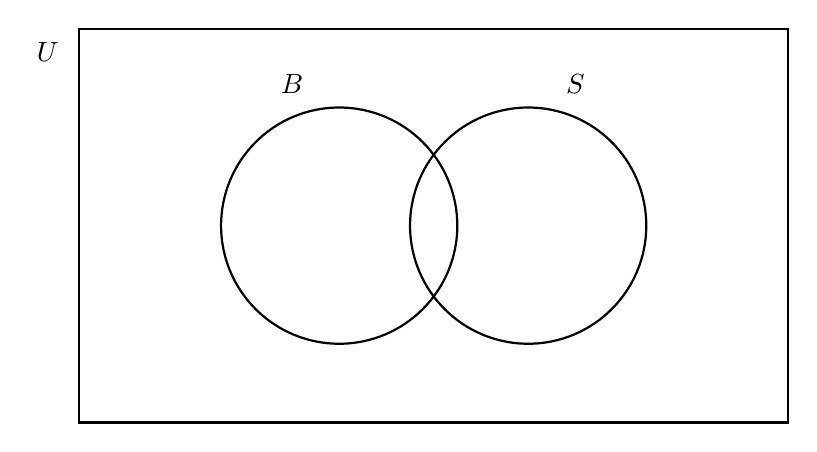
\begin{tikzpicture}
\draw[thick] (-2.5, -2.5) rectangle (6.5, 2.5);
\node at (-2.9, 2.2) {$U$};
\draw[thick] (0.8, 0) circle (1.5);
\draw[thick] (3.2, 0) circle (1.5);
\node at (0.2, 1.8) {$B$};
\node at (3.8, 1.8) {$S$};
\end{tikzpicture}
\end{center}
\phantom{.} \hfill \makebox[15pt][r]{[3]}
\item Find the number of students who do not own a bicycle.
\examanswerslot{2cm}{0.25}{1}
\end{enumerate}
\vspace{1cm}\par\noindent\rule{\linewidth}{0.4pt}\vspace{1cm}
\item \needspace{5cm}
Shade the required regions on the copies of the Venn diagrams provided below. \\
\begin{enumerate}[label=\textbf{(\alph*)}, leftmargin=*]
\item On the diagram, shade the region representing $A' \cap B$.
\begin{center}
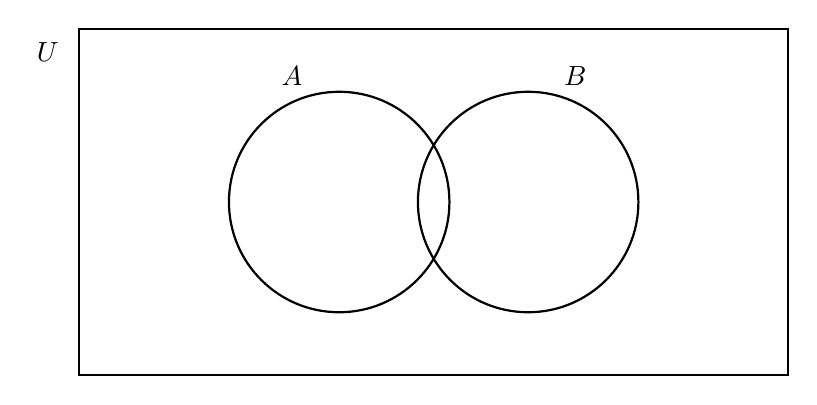
\begin{tikzpicture}
\draw[thick] (-2.5, -2.2) rectangle (6.5, 2.2);
\node at (-2.9, 1.9) {$U$};
\draw[thick] (0.8, 0) circle (1.4);
\draw[thick] (3.2, 0) circle (1.4);
\node at (0.2, 1.6) {$A$};
\node at (3.8, 1.6) {$B$};
\end{tikzpicture}
\end{center}
\phantom{.} \hfill \makebox[15pt][r]{[1]}
\item On the diagram, shade the region representing $(A \cup B)'$.
\begin{center}
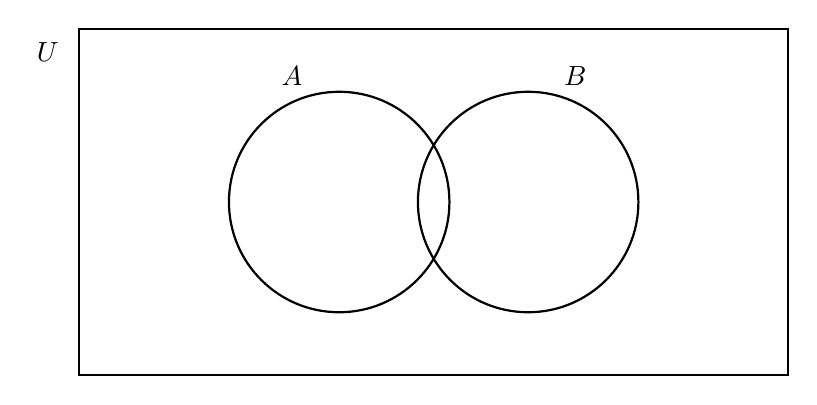
\begin{tikzpicture}
\draw[thick] (-2.5, -2.2) rectangle (6.5, 2.2);
\node at (-2.9, 1.9) {$U$};
\draw[thick] (0.8, 0) circle (1.4);
\draw[thick] (3.2, 0) circle (1.4);
\node at (0.2, 1.6) {$A$};
\node at (3.8, 1.6) {$B$};
\end{tikzpicture}
\end{center}
\phantom{.} \hfill \makebox[15pt][r]{[1]}
\end{enumerate}
\vspace{1cm}\par\noindent\rule{\linewidth}{0.4pt}\vspace{1cm}
\item The universal set $U$ is defined as $\{x \mid x \text{ is an integer and } 1 \le x \le 10\}$. \\
The sets $P$ and $Q$ are subsets of $U$ such that: \\
\par\vspace{0.1cm}\hspace*{0.6cm}$P = \{x \mid x \text{ is an even integer}\}$\par\vspace{0.15cm}
\par\vspace{0.1cm}\hspace*{0.6cm}$Q = \{x \mid x \text{ is a prime number}\}$\par\vspace{0.15cm}
\begin{enumerate}[label=\textbf{(\alph*)}, leftmargin=*]
\item Use a standard set notation symbol to complete the statement about the number 2 and the set $P$.
\par\vspace{0.1cm}\hspace*{0.6cm}$2 \dots\dots P$\par\vspace{0.15cm}
\examanswerslot{1.5cm}{0.25}{1}
\item List all the elements of the set $(P \cup Q)'$.
\examanswerslot{2cm}{0.25}{2}
\end{enumerate}
\vspace{1cm}\par\noindent\rule{\linewidth}{0.4pt}\vspace{1cm}
\item \needspace{5cm}
The Venn diagram shows the number of elements in each region for the sets $X$, $Y$, and $Z$. It is given that $\text{n}(U) = 45$. \\
\begin{center}
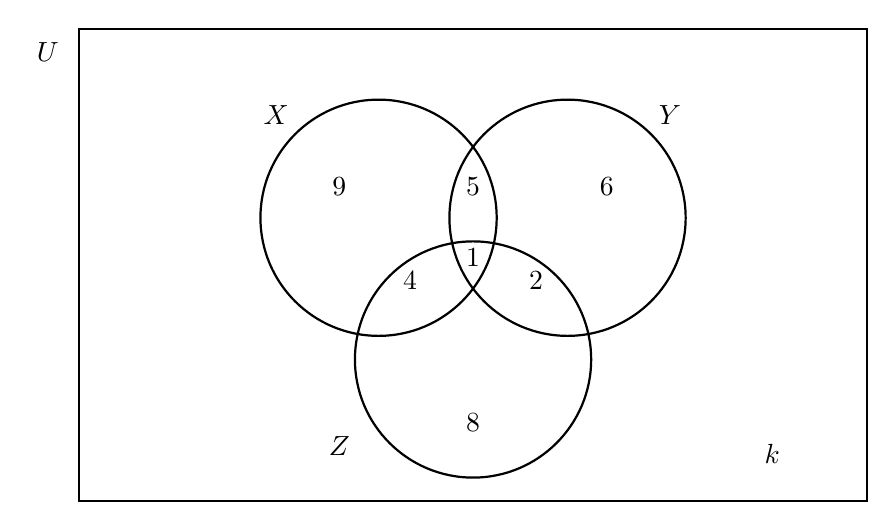
\begin{tikzpicture}
\draw[thick] (-3.0, -2.8) rectangle (7.0, 3.2);
\node at (-3.4, 2.9) {$U$};
\draw[thick] (0.8, 0.8) circle (1.5);
\draw[thick] (3.2, 0.8) circle (1.5);
\draw[thick] (2.0, -1.0) circle (1.5);
\node at (-0.5, 2.1) {$X$};
\node at (4.5, 2.1) {$Y$};
\node at (0.3, -2.1) {$Z$};
\node at (0.3, 1.2) {9};
\node at (3.7, 1.2) {6};
\node at (2.0, -1.8) {8};
\node at (2.0, 1.2) {5};
\node at (1.2, 0.0) {4};
\node at (2.8, 0.0) {2};
\node at (2.0, 0.3) {1};
\node at (5.8, -2.2) {$k$};
\end{tikzpicture}
\end{center}
\begin{enumerate}[label=\textbf{(\alph*)}, leftmargin=*]
\item Calculate the value of $k$.
\examanswerslot{2cm}{0.25}{2}
\item Find $\text{n}(X \cap Y \cap Z')$.
\examanswerslot{2cm}{0.25}{1}
\end{enumerate}
\vspace{1cm}\par\noindent\rule{\linewidth}{0.4pt}\vspace{1cm}
\item \needspace{5cm}
Shade the required regions on the copies of the Venn diagrams provided below. \\
\begin{enumerate}[label=\textbf{(\alph*)}, leftmargin=*]
\item On the diagram, shade the region representing $A \cap (B \cup C)'$.
\begin{center}
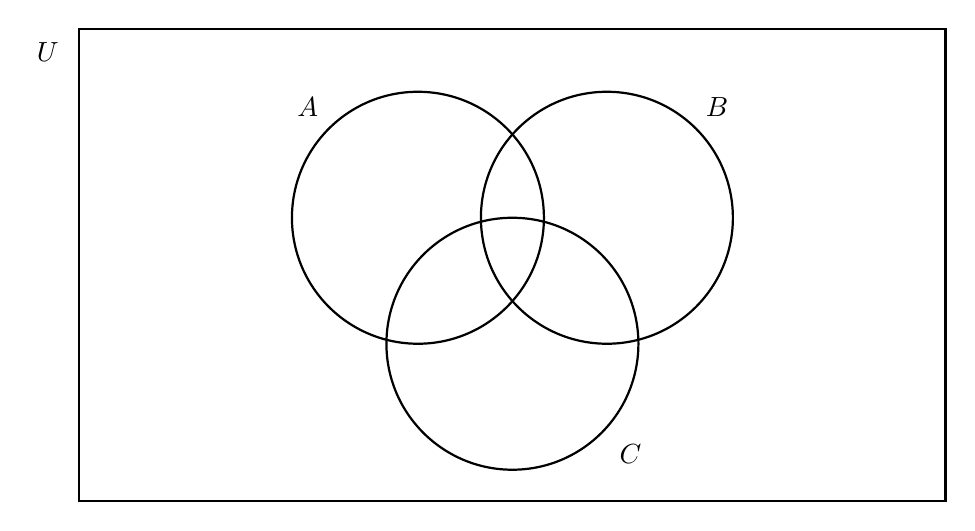
\begin{tikzpicture}
\draw[thick] (-5.5, -3.0) rectangle (5.5, 3.0);
\node at (-5.9, 2.7) {$U$};
\draw[thick] (-1.2, 0.6) circle (1.6);
\draw[thick] (1.2, 0.6) circle (1.6);
\draw[thick] (0, -1.0) circle (1.6);
\node at (-2.6, 2.0) {$A$};
\node at (2.6, 2.0) {$B$};
\node at (1.5, -2.4) {$C$};
\end{tikzpicture}
\end{center}
\phantom{.} \hfill \makebox[15pt][r]{[1]}
\item On the diagram, shade the region representing $(A \cap B)' \cap C$.
\begin{center}
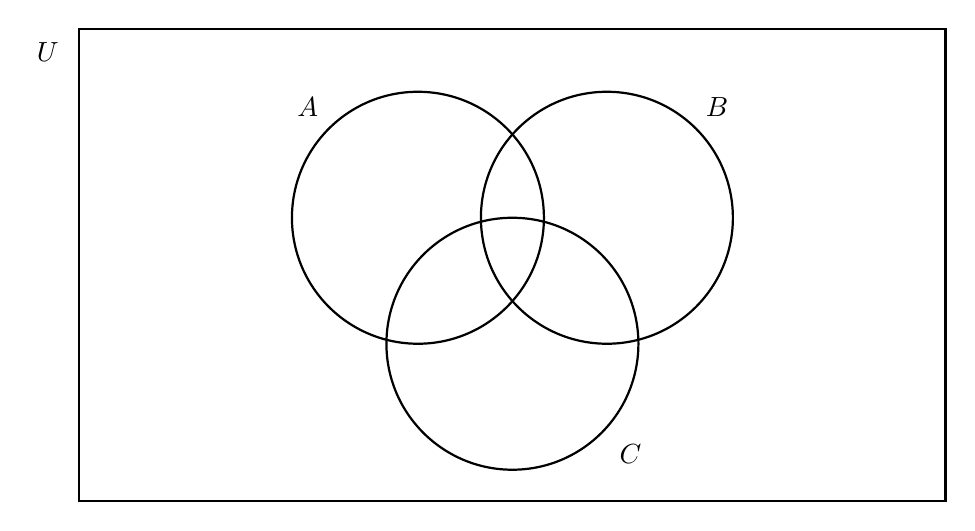
\begin{tikzpicture}
\draw[thick] (-5.5, -3.0) rectangle (5.5, 3.0);
\node at (-5.9, 2.7) {$U$};
\draw[thick] (-1.2, 0.6) circle (1.6);
\draw[thick] (1.2, 0.6) circle (1.6);
\draw[thick] (0, -1.0) circle (1.6);
\node at (-2.6, 2.0) {$A$};
\node at (2.6, 2.0) {$B$};
\node at (1.5, -2.4) {$C$};
\end{tikzpicture}
\end{center}
\phantom{.} \hfill \makebox[15pt][r]{[1]}
\end{enumerate}
\vspace{1cm}\par\noindent\rule{\linewidth}{0.4pt}\vspace{1cm}
\item \needspace{5cm}
A group of 40 students were asked if they like Mint chocolate ($M$) or Strawberry chocolate ($S$). \\
It is given that $\frac{1}{4}$ of the total number of students like both flavours, 6 students like neither flavour, and the number of students who like Mint only is twice the number of students who like Strawberry only. \\
\begin{enumerate}[label=\textbf{(\alph*)}, leftmargin=*]
\item Complete the Venn diagram to show the number of students in each region.
\begin{center}
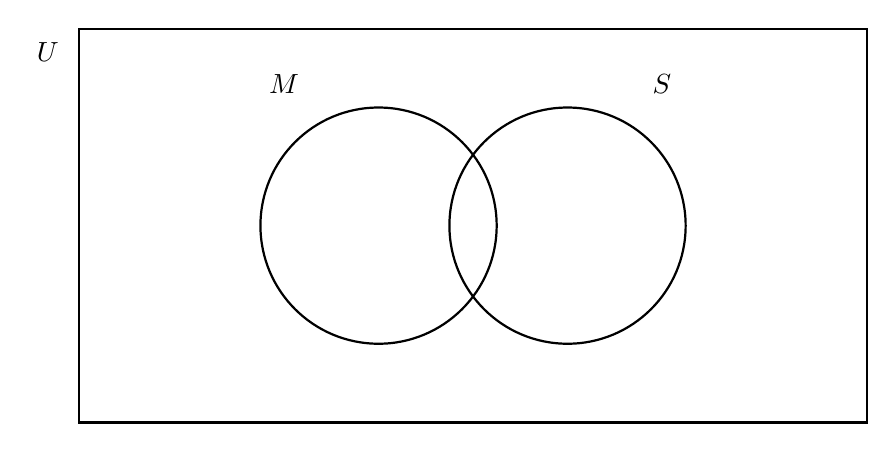
\begin{tikzpicture}
\draw[thick] (-5.0, -2.5) rectangle (5.0, 2.5);
\node at (-5.4, 2.2) {$U$};
\draw[thick] (-1.2, 0) circle (1.5);
\draw[thick] (1.2, 0) circle (1.5);
\node at (-2.4, 1.8) {$M$};
\node at (2.4, 1.8) {$S$};
\end{tikzpicture}
\end{center}
\phantom{.} \hfill \makebox[15pt][r]{[3]}
\item Find $\text{n}(M \cup S')$.
\examanswerslot{2cm}{0.25}{2}
\end{enumerate}
\vspace{1cm}\par\noindent\rule{\linewidth}{0.4pt}\vspace{1cm}
\item The universal set $U$ is defined as $\{x \mid x \text{ is a positive integer and } x \le 20\}$. \\
The sets $A$, $B$, and $C$ are subsets of $U$ defined as follows: \\
\par\vspace{0.1cm}\hspace*{0.6cm}$A = \{x \mid x \text{ is a multiple of 4}\}$\par\vspace{0.15cm}
\par\vspace{0.1cm}\hspace*{0.6cm}$B = \{x \mid x \text{ is a multiple of 8}\}$\par\vspace{0.15cm}
\par\vspace{0.1cm}\hspace*{0.6cm}$C = \{x \mid x \text{ is a factor of 20}\}$\par\vspace{0.15cm}
\begin{enumerate}[label=\textbf{(\alph*)}, leftmargin=*]
\item Complete the statement using the correct standard set notation symbol to describe the relationship between set $B$ and set $A$.
\par\vspace{0.1cm}\hspace*{0.6cm}$B \dots\dots A$\par\vspace{0.15cm}
\examanswerslot{1.5cm}{0.25}{1}
\item List all the elements of the set $(A \cap C) \cup B$.
\examanswerslot{2cm}{0.25}{2}
\end{enumerate}
\vspace{1cm}\par\noindent\rule{\linewidth}{0.4pt}\vspace{1cm}
\item The universal set $U$ has $\text{n}(U) = 78$. Two sets $P$ and $Q$ are defined within $U$ as follows: \\
\par\vspace{0.1cm}\hspace*{0.6cm}$P = \{y \mid y \in U \text{ and } y \text{ studies Physics}\}$\par\vspace{0.15cm}
\par\vspace{0.1cm}\hspace*{0.6cm}$Q = \{y \mid y \in U \text{ and } y \text{ studies Chemistry}\}$\par\vspace{0.15cm}
The number of elements in each specific region of the Venn diagram is given in terms of a positive integer $x$: \\
\par\vspace{0.1cm}\hspace*{0.6cm}$\text{n}(P \cap Q) = x^2 - 2x$\par\vspace{0.15cm}
\par\vspace{0.1cm}\hspace*{0.6cm}$\text{n}(P \cap Q') = 6x$\par\vspace{0.15cm}
\par\vspace{0.1cm}\hspace*{0.6cm}$\text{n}(Q \cap P') = 2x^2 - 5$\par\vspace{0.15cm}
\par\vspace{0.1cm}\hspace*{0.6cm}$\text{n}(P' \cap Q') = 3x + 7$\par\vspace{0.15cm}
\begin{enumerate}[label=\textbf{(\alph*)}, leftmargin=*]
\item Show that the equation for the total number of elements reduces to $3x^2 + 7x - 76 = 0$.
\examanswerslot{3.5cm}{0}{2}
\item Find $\text{n}(P' \cup Q)$.
\examanswerslot{2cm}{0.25}{3}
\end{enumerate}
\vspace{1cm}\par\noindent\rule{\linewidth}{0.4pt}\vspace{1cm}
\item \needspace{5cm}
On the independent Venn diagrams provided below, shade the precise region specified by each set expression. \\
\begin{enumerate}[label=\textbf{(\alph*)}, leftmargin=*]
\item Shade the region representing $(A \cap B') \cup (A' \cap B \cap C)$.
\begin{center}
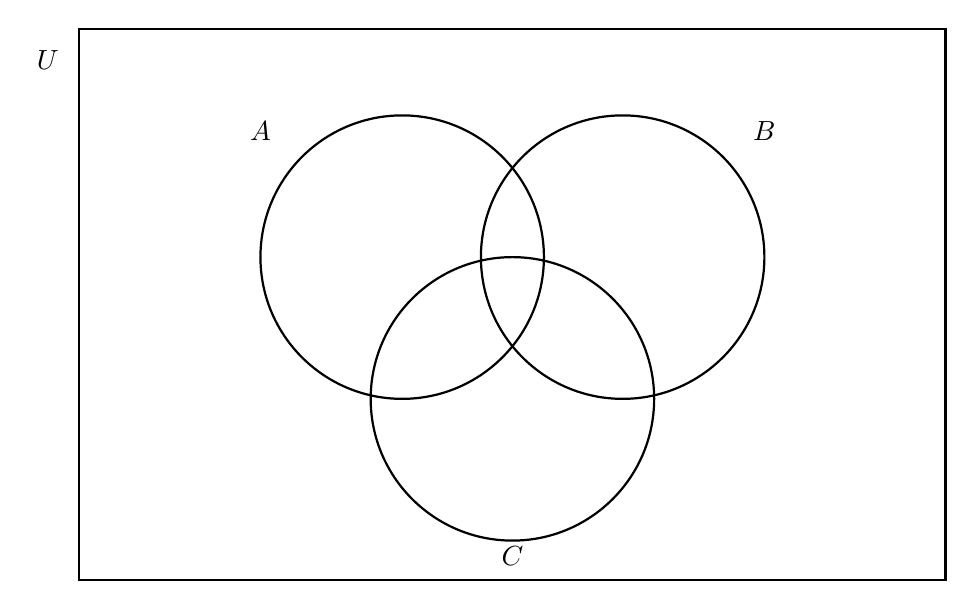
\begin{tikzpicture}
\draw[thick] (-5.5, -3.5) rectangle (5.5, 3.5);
\node at (-5.9, 3.1) {$U$};
\draw[thick] (-1.4, 0.6) circle (1.8);
\draw[thick] (1.4, 0.6) circle (1.8);
\draw[thick] (0, -1.2) circle (1.8);
\node at (-3.2, 2.2) {$A$};
\node at (3.2, 2.2) {$B$};
\node at (0, -3.2) {$C$};
\end{tikzpicture}
\end{center}
\phantom{.} \hfill \makebox[15pt][r]{[2]}
\item Shade the region representing $(A \cup C)' \cap B$.
\begin{center}
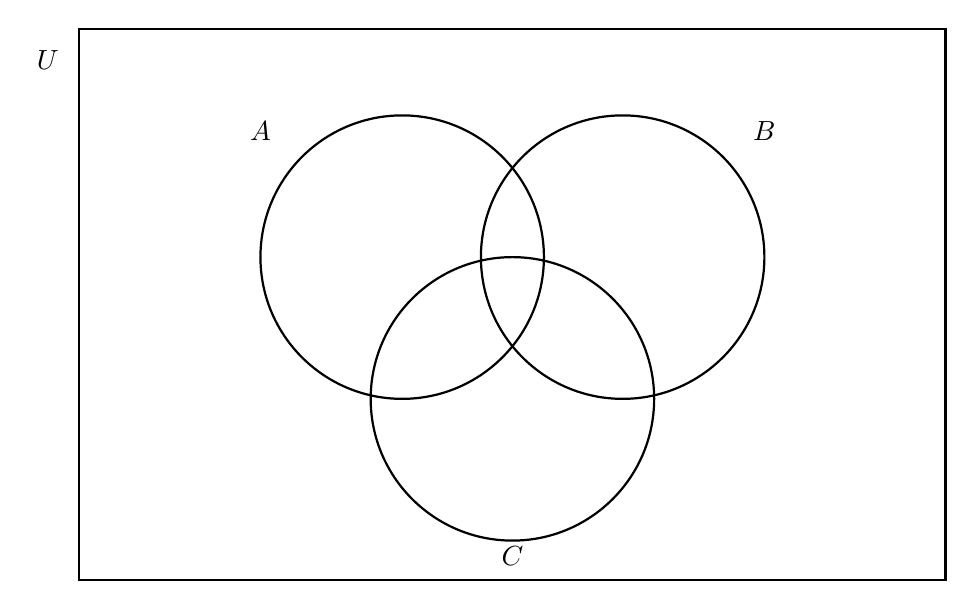
\begin{tikzpicture}
\draw[thick] (-5.5, -3.5) rectangle (5.5, 3.5);
\node at (-5.9, 3.1) {$U$};
\draw[thick] (-1.4, 0.6) circle (1.8);
\draw[thick] (1.4, 0.6) circle (1.8);
\draw[thick] (0, -1.2) circle (1.8);
\node at (-3.2, 2.2) {$A$};
\node at (3.2, 2.2) {$B$};
\node at (0, -3.2) {$C$};
\end{tikzpicture}
\end{center}
\phantom{.} \hfill \makebox[15pt][r]{[2]}
\end{enumerate}
\vspace{1cm}\par\noindent\rule{\linewidth}{0.4pt}\vspace{1cm}
\item \needspace{5cm}
A group of 100 students are surveyed about their participation in Athletics ($A$), Badminton ($B$), and Cricket ($C$). The results show that 38 students do Athletics, 34 students do Badminton, and 41 students do Cricket. The number of students in the intersection regions are described in terms of $x$: \\
* $x$ students participate in all three sports. \\
* The number of students who do Badminton and Cricket only is $2x$. \\
* The number of students who do Athletics and Cricket only is $x + 1$. \\
* The number of students who do Athletics and Badminton only is $2x - 3$. \\
* The number of students who do Cricket only is equal to the number of students who do none of the three sports. \\
\begin{enumerate}[label=\textbf{(\alph*)}, leftmargin=*]
\item Formulate an equation in terms of $x$ for the total number of students and show that it reduces to $155 - 11x = 100$.
\examanswerslot{3.5cm}{0}{3}
\item Complete the Venn diagram to show the exact number of students in each of the 8 regions.
\begin{center}
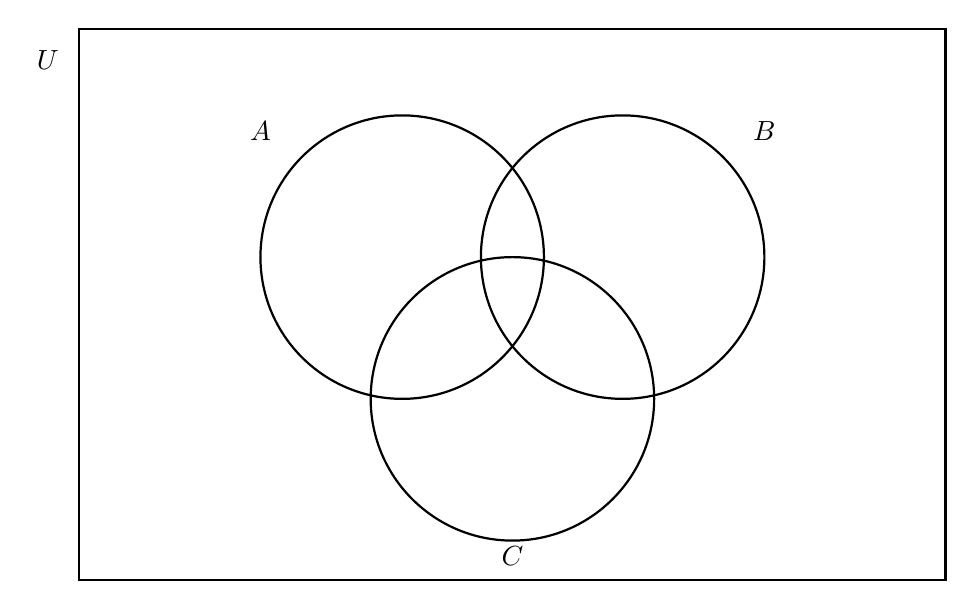
\begin{tikzpicture}
\draw[thick] (-5.5, -3.5) rectangle (5.5, 3.5);
\node at (-5.9, 3.1) {$U$};
\draw[thick] (-1.4, 0.6) circle (1.8);
\draw[thick] (1.4, 0.6) circle (1.8);
\draw[thick] (0, -1.2) circle (1.8);
\node at (-3.2, 2.2) {$A$};
\node at (3.2, 2.2) {$B$};
\node at (0, -3.2) {$C$};
\end{tikzpicture}
\end{center}
\phantom{.} \hfill \makebox[15pt][r]{[3]}
\end{enumerate}
\vspace{1cm}\par\noindent\rule{\linewidth}{0.4pt}\vspace{1cm}
\item The universal set $U$ is defined as: \\
\par\vspace{0.1cm}\hspace*{0.6cm}$U = \{x \mid x \text{ is an integer and } 1 \le x \le 30\}$\par\vspace{0.15cm}
Three subsets $A$, $B$, and $C$ are defined within $U$ as follows: \\
\par\vspace{0.1cm}\hspace*{0.6cm}$A = \{x \mid x \in U \text{ and } x \text{ is a multiple of 3}\}$\par\vspace{0.15cm}
\par\vspace{0.1cm}\hspace*{0.6cm}$B = \{x \mid x \in U \text{ and } x \text{ is a multiple of 4}\}$\par\vspace{0.15cm}
\par\vspace{0.1cm}\hspace*{0.6cm}$C = \{x \mid x \in U \text{ and } x \text{ is a perfect square}\}$\par\vspace{0.15cm}
\begin{enumerate}[label=\textbf{(\alph*)}, leftmargin=*]
\item State whether the statement $C \subseteq (A' \cap B')'$ is true or false. Justify your answer explicitly by identifying the elements that support your conclusion.
\examanswerslot{3.5cm}{0}{2}
\item Calculate $\text{n}((A \cap B') \cup (B \cap C'))$.
\examanswerslot{2cm}{0.25}{2}
\end{enumerate}
\vspace{1cm}\par\noindent\rule{\linewidth}{0.4pt}\vspace{1cm}
\item \needspace{5cm}
The Venn diagram shows the number of elements in three sets, $A$, $B$, and $C$. \\
\begin{center}
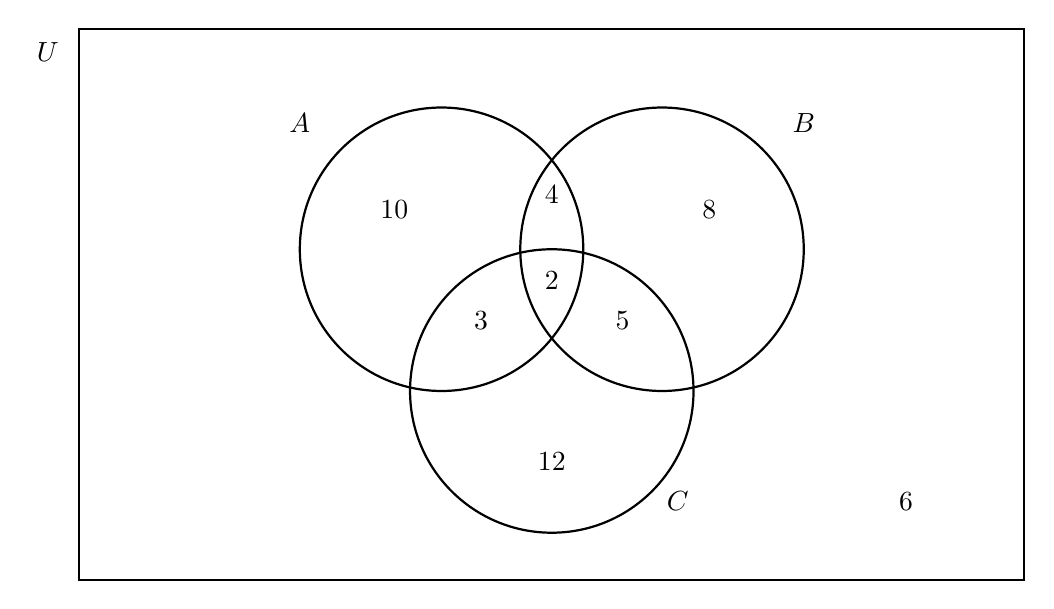
\begin{tikzpicture}
\draw[thick] (-6.0, -3.5) rectangle (6.0, 3.5);
\node at (-6.4, 3.2) {$U$};
\draw[thick] (-1.4, 0.7) circle (1.8);
\draw[thick] (1.4, 0.7) circle (1.8);
\draw[thick] (0, -1.1) circle (1.8);
\node at (-3.2, 2.3) {$A$};
\node at (3.2, 2.3) {$B$};
\node at (1.6, -2.5) {$C$};
\node at (-2.0, 1.2) {10};
\node at (2.0, 1.2) {8};
\node at (0, -2.0) {12};
\node at (0, 1.4) {4};
\node at (-0.9, -0.2) {3};
\node at (0.9, -0.2) {5};
\node at (0, 0.3) {2};
\node at (4.5, -2.5) {6};
\end{tikzpicture}
\end{center}
\begin{enumerate}[label=\textbf{(\alph*)}, leftmargin=*]
\item Find $\text{n}(A \cap B)$.
\examanswerslot{2cm}{0.25}{1}
\item Find $\text{n}(A \cup C)$.
\examanswerslot{2cm}{0.25}{2}
\end{enumerate}
\vspace{1cm}\par\noindent\rule{\linewidth}{0.4pt}\vspace{1cm}
\item \needspace{5cm}
On the independent Venn diagrams provided below, shade the precise region specified by each set expression. \\
\begin{enumerate}[label=\textbf{(\alph*)}, leftmargin=*]
\item On the diagram, shade the region representing $A \cap B \cap C'$.
\begin{center}
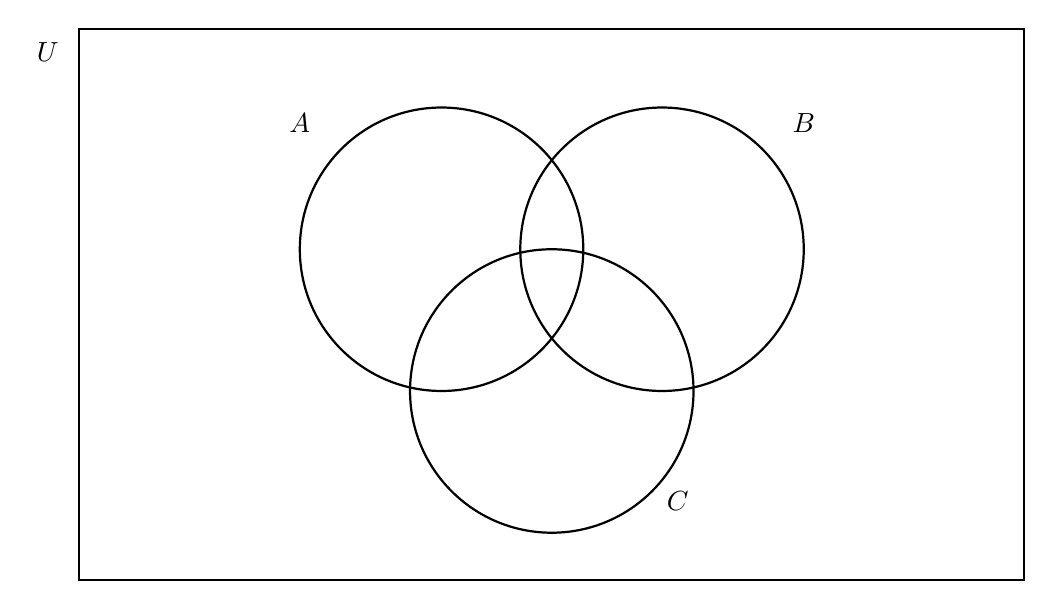
\begin{tikzpicture}
\draw[thick] (-6.0, -3.5) rectangle (6.0, 3.5);
\node at (-6.4, 3.2) {$U$};
\draw[thick] (-1.4, 0.7) circle (1.8);
\draw[thick] (1.4, 0.7) circle (1.8);
\draw[thick] (0, -1.1) circle (1.8);
\node at (-3.2, 2.3) {$A$};
\node at (3.2, 2.3) {$B$};
\node at (1.6, -2.5) {$C$};
\end{tikzpicture}
\end{center}
\phantom{.} \hfill \makebox[15pt][r]{[1]}
\item On the diagram, shade the region representing $(A \cup B)' \cap C$.
\begin{center}
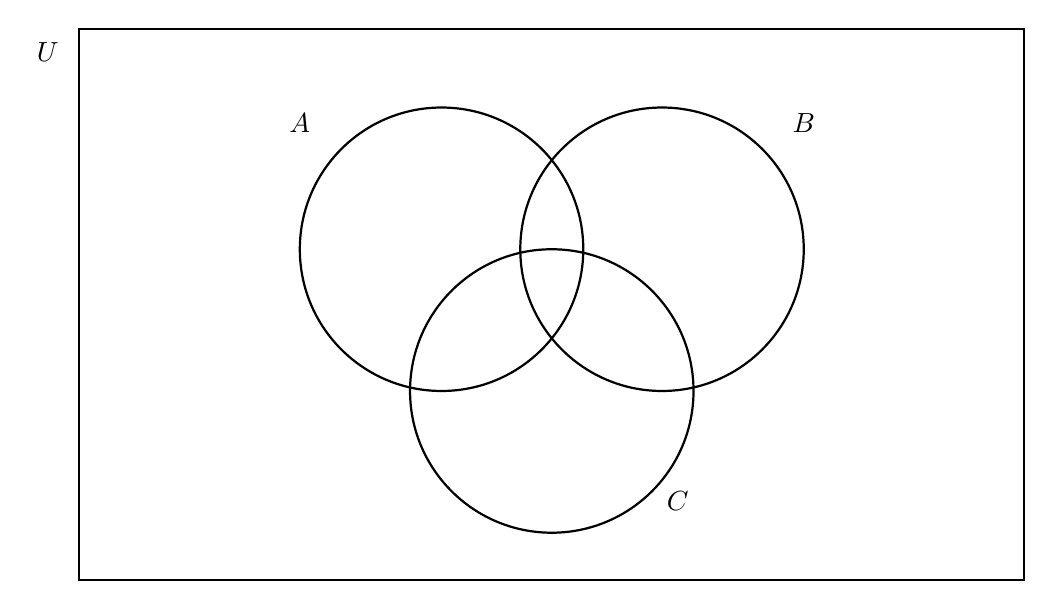
\begin{tikzpicture}
\draw[thick] (-6.0, -3.5) rectangle (6.0, 3.5);
\node at (-6.4, 3.2) {$U$};
\draw[thick] (-1.4, 0.7) circle (1.8);
\draw[thick] (1.4, 0.7) circle (1.8);
\draw[thick] (0, -1.1) circle (1.8);
\node at (-3.2, 2.3) {$A$};
\node at (3.2, 2.3) {$B$};
\node at (1.6, -2.5) {$C$};
\end{tikzpicture}
\end{center}
\phantom{.} \hfill \makebox[15pt][r]{[1]}
\end{enumerate}
\vspace{1cm}\par\noindent\rule{\linewidth}{0.4pt}\vspace{1cm}
\item \needspace{5cm}
A survey of 50 people found that 28 speak Spanish ($S$) and 25 speak French ($F$). There are 8 people who speak neither language. \\
\begin{enumerate}[label=\textbf{(\alph*)}, leftmargin=*]
\item Complete the Venn diagram to show the number of people in each region.
\begin{center}
\begin{tikzpicture}
\draw[thick] (-6.0, -3.5) rectangle (6.0, 3.5);
\node at (-6.4, 3.2) {$U$};
\draw[thick] (-1.5, 0) circle (1.8);
\draw[thick] (1.5, 0) circle (1.8);
\node at (-2.8, 2.0) {$S$};
\node at (2.8, 2.0) {$F$};
\end{tikzpicture}
\end{center}
\phantom{.} \hfill \makebox[15pt][r]{[3]}
\item Find the number of people who speak Spanish but do not speak French.
\examanswerslot{2cm}{0.25}{1}
\end{enumerate}
\vspace{1cm}\par\noindent\rule{\linewidth}{0.4pt}\vspace{1cm}
\item \begin{enumerate}[label=\textbf{(\alph*)}, leftmargin=*]
\item Write the number four million five hundred thousand and twenty-six in figures.
\examanswerslot{2cm}{0.25}{1}
\item From the following list of numbers:
\par\vspace{0.1cm}\hspace*{0.6cm}$\sqrt{7}, \quad 9, \quad 15, \quad 23, \quad 28, \quad 36$\par\vspace{0.15cm}
identify: \\
\begin{enumerate}[label=\textbf{(\roman*)}, leftmargin=0.6cm]
\item the prime number,
\examanswerslot{2cm}{0.25}{1}
\item the square number that is also a multiple of 4,
\examanswerslot{2cm}{0.25}{1}
\item the irrational number.
\examanswerslot{2cm}{0.25}{1}
\end{enumerate}
\end{enumerate}
\vspace{1cm}\par\noindent\rule{\linewidth}{0.4pt}\vspace{1cm}
\item Two numbers are given as $A = 2^2 \times 3 \times 5$ and $B = 2 \times 3^2 \times 7$. \\
\begin{enumerate}[label=\textbf{(\alph*)}, leftmargin=*]
\item Find the Highest Common Factor (HCF) of $A$ and $B$.
\examanswerslot{2cm}{0.25}{2}
\item Find the Lowest Common Multiple (LCM) of $A$ and $B$. Give your answer as an integer.
\examanswerslot{2cm}{0.25}{2}
\end{enumerate}
\vspace{1cm}\par\noindent\rule{\linewidth}{0.4pt}\vspace{1cm}
\item \begin{enumerate}[label=\textbf{(\alph*)}, leftmargin=*]
\item Express 72 as a product of its prime factors. Give your answer in index form.
\examanswerslot{2cm}{0.25}{2}
\item Write down the reciprocal of 72.
\examanswerslot{2cm}{0.25}{1}
\end{enumerate}
\vspace{1cm}\par\noindent\rule{\linewidth}{0.4pt}\vspace{1cm}
\item Consider the algebraic terms $X = 12a^2b$ and $Y = 30ab^3$, where $a$ and $b$ are distinct prime numbers. \\
\begin{enumerate}[label=\textbf{(\alph*)}, leftmargin=*]
\item Find the Highest Common Factor (HCF) of $X$ and $Y$ in terms of $a$ and $b$.
\examanswerslot{2cm}{0.25}{2}
\item Find the Lowest Common Multiple (LCM) of $X$ and $Y$ in terms of $a$ and $b$.
\examanswerslot{2cm}{0.25}{2}
\end{enumerate}
\vspace{1cm}\par\noindent\rule{\linewidth}{0.4pt}\vspace{1cm}
\item \begin{enumerate}[label=\textbf{(\alph*)}, leftmargin=*]
\item Write the number 30 040 008 in words using British standard formatting.
\examanswerslot{3cm}{0.25}{1}
\item Find the Highest Common Factor (HCF) of 45 and 105.
\examanswerslot{2cm}{0.25}{2}
\end{enumerate}
\vspace{1cm}\par\noindent\rule{\linewidth}{0.4pt}\vspace{1cm}
\item \begin{enumerate}[label=\textbf{(\alph*)}, leftmargin=*]
\item Write the number forty-two billion seven hundred million and four in figures.
\examanswerslot{2cm}{0.25}{1}
\item From the following list of numbers:
\par\vspace{0.1cm}\hspace*{0.6cm}$\sqrt{16}, \quad 27, \quad \frac{2}{3}, \quad \pi, \quad 28, \quad 45$\par\vspace{0.15cm}
identify: \\
\begin{enumerate}[label=\textbf{(\roman*)}, leftmargin=0.6cm]
\item the cube number,
\examanswerslot{2cm}{0.25}{1}
\item the triangle number,
\examanswerslot{2cm}{0.25}{1}
\item the irrational number.
\examanswerslot{2cm}{0.25}{1}
\end{enumerate}
\end{enumerate}
\vspace{1cm}\par\noindent\rule{\linewidth}{0.4pt}\vspace{1cm}
\item \begin{enumerate}[label=\textbf{(\alph*)}, leftmargin=*]
\item Express 540 as a product of its prime factors. Give your answer in index form.
\examanswerslot{2cm}{0.25}{2}
\item Given that $540 \times k$ is a perfect square, where $k$ is a positive integer, find the smallest possible value of $k$.
\examanswerslot{2cm}{0.25}{2}
\item Write down the reciprocal of $k$.
\examanswerslot{2cm}{0.25}{1}
\end{enumerate}
\vspace{1cm}\par\noindent\rule{\linewidth}{0.4pt}\vspace{1cm}
\item Two numbers, $X$ and $Y$, are expressed as products of their prime factors: \\
\par\vspace{0.1cm}\hspace*{0.6cm}$X = 2^3 \times 3^2 \times 5 \times 11$\par\vspace{0.15cm}
\par\vspace{0.1cm}\hspace*{0.6cm}$Y = 2^2 \times 3^4 \times 7$\par\vspace{0.15cm}
\begin{enumerate}[label=\textbf{(\alph*)}, leftmargin=*]
\item Find the Highest Common Factor (HCF) of $X$ and $Y$. Give your answer as an integer.
\examanswerslot{2cm}{0.25}{2}
\item Find the Lowest Common Multiple (LCM) of $X$ and $Y$. Give your answer in index form.
\examanswerslot{2cm}{0.25}{2}
\end{enumerate}
\vspace{1cm}\par\noindent\rule{\linewidth}{0.4pt}\vspace{1cm}
\item A security light flashes every 42 seconds. A second security light flashes every 60 seconds. Both lights flash together at 19:30. \\
\begin{enumerate}[label=\textbf{(\alph*)}, leftmargin=*]
\item Find the Lowest Common Multiple (LCM) of 42 and 60.
\examanswerslot{2cm}{0.25}{2}
\item Determine the next time both lights will flash together.
\examanswerslot{2cm}{0.25}{2}
\end{enumerate}
\vspace{1cm}\par\noindent\rule{\linewidth}{0.4pt}\vspace{1cm}
\item \begin{enumerate}[label=\textbf{(\alph*)}, leftmargin=*]
\item Write the number thirteen billion two hundred million and five in figures.
\examanswerslot{2cm}{0.25}{1}
\item A number $N$ is expressed as the product of its prime factors as:
\par\vspace{0.1cm}\hspace*{0.6cm}$N = 2^{x} \times 3^{y} \times 5^{z}$\par\vspace{0.15cm}
The reciprocal of $N$ has an indexing layout. Given that $N$ is a perfect cube, a perfect square, and a multiple of 10, find the smallest possible integer value of $N$. Give your answer in index form. \\
\examanswerslot{2cm}{0.25}{2}
\item From the following set of numbers:
\par\vspace{0.1cm}\hspace*{0.6cm}$\left\{ \sqrt[3]{27}, \  \sqrt{8}, \  \frac{22}{7}, \  0.1313313331\ldots, \  T_{10} \right\}$\par\vspace{0.15cm}
where $T_{10}$ represents the 10th triangle number, identify: \\
\begin{enumerate}[label=\textbf{(\roman*)}, leftmargin=0.6cm]
\item the value of the triangle number $T_{10}$,
\examanswerslot{2cm}{0.25}{1}
\item all the irrational numbers in the set.
\examanswerslot{2cm}{0.25}{1}
\end{enumerate}
\end{enumerate}
\vspace{1cm}\par\noindent\rule{\linewidth}{0.4pt}\vspace{1cm}
\item Two algebraic terms, $P$ and $Q$, are defined below, where $x$, $y$, and $z$ are distinct prime numbers. \\
\par\vspace{0.1cm}\hspace*{0.6cm}$P = 126x^4y^2z^3$\par\vspace{0.15cm}
\par\vspace{0.1cm}\hspace*{0.6cm}$Q = 540x^2y^5$\par\vspace{0.15cm}
\begin{enumerate}[label=\textbf{(\alph*)}, leftmargin=*]
\item Express 126 and 540 as products of their prime factors.
\examanswerslot{2cm}{0.25}{2}
\item Find the Highest Common Factor (HCF) of $P$ and $Q$ in terms of $x$, $y$, and $z$.
\examanswerslot{2cm}{0.25}{2}
\item Find the Lowest Common Multiple (LCM) of $P$ and $Q$ in terms of $x$, $y$, and $z$. Give your coefficient as an integer.
\examanswerslot{2cm}{0.25}{2}
\end{enumerate}
\vspace{1cm}\par\noindent\rule{\linewidth}{0.4pt}\vspace{1cm}
\item Three integers are given as $A = 2^3 \times 3^x \times 5^2$, $B = 2^y \times 3^2 \times 7$, and $C = 3^3 \times 5^z \times 11$. \\
\begin{enumerate}[label=\textbf{(\alph*)}, leftmargin=*]
\item Given that the Highest Common Factor of $A$ and $B$ is $\text{HCF}(A, B) = 36$, find the exact values of the exponents $x$ and $y$.
\examanswerslot{2cm}{0.25}{2}
\item Given that the Lowest Common Multiple of $A$ and $C$ is $\text{LCM}(A, C) = 2^3 \times 3^4 \times 5^3 \times 11$, find the exact values of the exponents $x$ and $z$.
\examanswerslot{2cm}{0.25}{2}
\item State whether the number $\frac{A \times B}{C}$ is rational or irrational when $x=2, y=2, z=1$.
\examanswerslot{2cm}{0.25}{1}
\end{enumerate}
\vspace{1cm}\par\noindent\rule{\linewidth}{0.4pt}\vspace{1cm}
\item \begin{enumerate}[label=\textbf{(\alph*)}, leftmargin=*]
\item Write the number 'five billion two hundred million and seventy-three' in figures.
\examanswerslot{2cm}{0.25}{1}
\item Consider the following list of real numbers:
\par\vspace{0.1cm}\hspace*{0.6cm}$\sqrt{5}, \quad 16, \quad 27, \quad 28, \quad \frac{7}{9}, \quad 41$\par\vspace{0.15cm}
Identify from the list: \\
\begin{enumerate}[label=\textbf{(\roman*)}, leftmargin=0.6cm]
\item the prime number,
\examanswerslot{2cm}{0.25}{1}
\item the cube number,
\examanswerslot{2cm}{0.25}{1}
\item the triangle number.
\examanswerslot{2cm}{0.25}{1}
\end{enumerate}
\end{enumerate}
\vspace{1cm}\par\noindent\rule{\linewidth}{0.4pt}\vspace{1cm}
\item \begin{enumerate}[label=\textbf{(\alph*)}, leftmargin=*]
\item Express the integer 360 as a product of its prime factors. Give your final answer in index form.
\examanswerslot{2cm}{0.25}{2}
\item Write down the exact value of the reciprocal of 360.
\examanswerslot{2cm}{0.25}{1}
\end{enumerate}
\vspace{1cm}\par\noindent\rule{\linewidth}{0.4pt}\vspace{1cm}
\item Two numbers are given as $P = 2^3 \times 3 \times 5^2$ and $Q = 2 \times 3^2 \times 5$. \\
\begin{enumerate}[label=\textbf{(\alph*)}, leftmargin=*]
\item Find the Highest Common Factor (HCF) of $P$ and $Q$. Give your answer as an integer.
\examanswerslot{2cm}{0.25}{2}
\item Find the Lowest Common Multiple (LCM) of $P$ and $Q$. Give your answer as an integer.
\examanswerslot{2cm}{0.25}{2}
\end{enumerate}
\vspace{1cm}\par\noindent\rule{\linewidth}{0.4pt}\vspace{1cm}
\item Consider the simple algebraic expressions $M = 14x^2y$ and $N = 35xy^3$, where $x$ and $y$ are distinct prime numbers. \\
\begin{enumerate}[label=\textbf{(\alph*)}, leftmargin=*]
\item Find the Highest Common Factor (HCF) of $M$ and $N$ in terms of $x$ and $y$.
\examanswerslot{2cm}{0.25}{2}
\item Find the Lowest Common Multiple (LCM) of $M$ and $N$ in terms of $x$ and $y$.
\examanswerslot{2cm}{0.25}{2}
\end{enumerate}
\vspace{1cm}\par\noindent\rule{\linewidth}{0.4pt}\vspace{1cm}
\item \begin{enumerate}[label=\textbf{(\alph*)}, leftmargin=*]
\item A specific natural number $W$ is described in words as 'two billion four hundred and eighty-four million'. Express $W$ as a product of its prime factors using index form.
\examanswerslot{2.5cm}{0.25}{3}
\item A statistical tracking variable $V$ updates continuous sample bins. The value of $V$ is given by:
\par\vspace{0.1cm}\hspace*{0.6cm}$V = \frac{W \times 10^4}{2 \times 3^3 \times 5^6}$\par\vspace{0.15cm}
Evaluate the expression to show that $V$ is a perfect square number. \\
\examanswerslot{3.5cm}{0}{3}
\end{enumerate}
\vspace{1cm}\par\noindent\rule{\linewidth}{0.4pt}\vspace{1cm}
\item Two complex variables inside a digital geometric rendering algorithm are defined by the prime factor layouts: \\
\par\vspace{0.1cm}\hspace*{0.6cm}$X = 2^a \times 3^4 \times 5^2 \times y^3$\par\vspace{0.15cm}
\par\vspace{0.1cm}\hspace*{0.6cm}$Y = 2^3 \times 3^b \times 5^c \times z^2$\par\vspace{0.15cm}
where $y$ and $z$ are distinct, unknown prime numbers greater than 5, and $a$, $b$, and $c$ are integers. \\
\begin{enumerate}[label=\textbf{(\alph*)}, leftmargin=*]
\item Given that $\text{HCF}(X, Y) = 360$, calculate the exact values of $a$, $b$, and $c$.
\examanswerslot{2cm}{0.25}{3}
\item Given that $\text{LCM}(X,Y) = 2.43 \times 10^7$, write down a mathematical equation relating the prime variables $y$ and $z$.
\examanswerslot{2cm}{0.25}{2}
\end{enumerate}
\vspace{1cm}\par\noindent\rule{\linewidth}{0.4pt}\vspace{1cm}
\item A continuous automated monitoring station tracks data packet volumes transmitted across a global telecommunications network. \\
\begin{enumerate}[label=\textbf{(\alph*)}, leftmargin=*]
\item At peak capacity, one key transmission link records a data volume of thirty-four billion eight hundred million and ninety-two bytes per hour. Write this numerical quantity in figures.
\examanswerslot{2cm}{0.25}{1}
\item A structural routing constant $K$ is measured across the network data nodes and belongs to the following given set of numbers:
\par\vspace{0.1cm}\hspace*{0.6cm}$\left\{ \sqrt{18}, \quad 64, \quad \frac{22}{7}, \quad 45, \quad 53 \right\}$\par\vspace{0.15cm}
Identify from this set: \\
\begin{enumerate}[label=\textbf{(\roman*)}, leftmargin=0.6cm]
\item the prime number,
\examanswerslot{2cm}{0.25}{1}
\item the square number that is also a cube number,
\examanswerslot{2cm}{0.25}{1}
\item the irrational number.
\examanswerslot{2cm}{0.25}{1}
\end{enumerate}
\end{enumerate}
\vspace{1cm}\par\noindent\rule{\linewidth}{0.4pt}\vspace{1cm}
\item A multi-stage mechanical sorting conveyor uses two large independent primary driving wheels. The structural indices for the tooth configurations are represented by the variables $A$ and $B$, where: \\
\par\vspace{0.1cm}\hspace*{0.6cm}$A = 2^4 \times 3^2 \times 5 \times 11$\par\vspace{0.15cm}
\par\vspace{0.1cm}\hspace*{0.6cm}$B = 2^2 \times 3^3 \times 5^2 \times 7$\par\vspace{0.15cm}
\begin{enumerate}[label=\textbf{(\alph*)}, leftmargin=*]
\item Calculate the Highest Common Factor (HCF) of $A$ and $B$. Give your answer as an exact integer.
\examanswerslot{2cm}{0.25}{2}
\item Calculate the Lowest Common Multiple (LCM) of $A$ and $B$. Give your answer as a calculation evaluated to 3 significant figures, expressed in standard scientific notation.
\examanswerslot{2cm}{0.25}{2}
\end{enumerate}
\vspace{1cm}\par\noindent\rule{\linewidth}{0.4pt}\vspace{1cm}
\item An astronomical monitoring facility models periodic cycles of digital telemetry feeds. Satellite Alpha transmits data packets every 1.75 minutes, while Satellite Beta transmits packets every 2.25 minutes. Both systems log initial concurrent data pings at exactly 04:00. \\
\begin{enumerate}[label=\textbf{(\alph*)}, leftmargin=*]
\item Convert the time cycles into simple written fractions of minutes, and find the precise Lowest Common Multiple (LCM) of the periodic cycles for Satellite Alpha and Satellite Beta.
\examanswerslot{2cm}{0.25}{2}
\item Calculate the total elapsed time in minutes, and determine the next exact time on a 24-hour clock when both satellites will transmit simultaneously.
\examanswerslot{2cm}{0.25}{2}
\end{enumerate}
\vspace{1cm}\par\noindent\rule{\linewidth}{0.4pt}\vspace{1cm}
\item \begin{enumerate}[label=\textbf{(\alph*)}, leftmargin=*]
\item Evaluate the expression.
\par\vspace{0.1cm}\hspace*{0.6cm}$5^2 \times \sqrt[3]{8}$\par\vspace{0.15cm}
\examanswerslot{2cm}{0.25}{2}
\item Evaluate the expression.
\par\vspace{0.1cm}\hspace*{0.6cm}$10^3 - \sqrt{144}$\par\vspace{0.15cm}
\examanswerslot{2cm}{0.25}{2}
\end{enumerate}
\vspace{1cm}\par\noindent\rule{\linewidth}{0.4pt}\vspace{1cm}
\item \begin{enumerate}[label=\textbf{(\alph*)}, leftmargin=*]
\item Evaluate the expression.
\par\vspace{0.1cm}\hspace*{0.6cm}$\sqrt{121} + 3^3 \times \sqrt[3]{1}$\par\vspace{0.15cm}
\examanswerslot{2cm}{0.25}{2}
\item Evaluate the expression.
\par\vspace{0.1cm}\hspace*{0.6cm}$\dfrac{2^3 \times \sqrt{169}}{10^2 - 96}$\par\vspace{0.15cm}
\examanswerslot{2cm}{0.25}{2}
\end{enumerate}
\vspace{1cm}\par\noindent\rule{\linewidth}{0.4pt}\vspace{1cm}
\item \begin{enumerate}[label=\textbf{(\alph*)}, leftmargin=*]
\item Evaluate the expression.
\par\vspace{0.1cm}\hspace*{0.6cm}$\sqrt[3]{64} \times 4^2 - \sqrt{225}$\par\vspace{0.15cm}
\examanswerslot{2cm}{0.25}{2}
\item Evaluate the expression.
\par\vspace{0.1cm}\hspace*{0.6cm}$\dfrac{\sqrt{196}}{\sqrt[3]{8}} + 12^2$\par\vspace{0.15cm}
\examanswerslot{2cm}{0.25}{2}
\end{enumerate}
\vspace{1cm}\par\noindent\rule{\linewidth}{0.4pt}\vspace{1cm}
\item \begin{enumerate}[label=\textbf{(\alph*)}, leftmargin=*]
\item Evaluate the expression.
\par\vspace{0.1cm}\hspace*{0.6cm}$2 \times \sqrt{81} - 3^2 \times \sqrt[3]{27}$\par\vspace{0.15cm}
\examanswerslot{2cm}{0.25}{2}
\item Evaluate the expression.
\par\vspace{0.1cm}\hspace*{0.6cm}$\sqrt{100} \times \sqrt{4} - 5^3$\par\vspace{0.15cm}
\examanswerslot{2cm}{0.25}{2}
\end{enumerate}
\vspace{1cm}\par\noindent\rule{\linewidth}{0.4pt}\vspace{1cm}
\item \begin{enumerate}[label=\textbf{(\alph*)}, leftmargin=*]
\item Convert $0.35$ into a proper fraction written in its simplest form.
\examanswerslot{2cm}{0.25}{1}
\item Convert $\dfrac{7}{20}$ into a percentage.
\examanswerslot{2cm}{0.25}{1}
\end{enumerate}
\vspace{1cm}\par\noindent\rule{\linewidth}{0.4pt}\vspace{1cm}
\item \begin{enumerate}[label=\textbf{(\alph*)}, leftmargin=*]
\item Convert $12.5\%$ into a fraction written in its simplest form.
\examanswerslot{2cm}{0.25}{1}
\item Write the mixed number $2\dfrac{3}{5}$ as a decimal number.
\examanswerslot{2cm}{0.25}{1}
\end{enumerate}
\vspace{1cm}\par\noindent\rule{\linewidth}{0.4pt}\vspace{1cm}
\item \begin{enumerate}[label=\textbf{(\alph*)}, leftmargin=*]
\item Convert the improper fraction $\dfrac{14}{4}$ into a mixed number in its simplest form.
\examanswerslot{2cm}{0.25}{1}
\item Convert your answer from part (a) into a decimal.
\examanswerslot{2cm}{0.25}{1}
\end{enumerate}
\vspace{1cm}\par\noindent\rule{\linewidth}{0.4pt}\vspace{1cm}
\item \begin{enumerate}[label=\textbf{(\alph*)}, leftmargin=*]
\item Express $0.08$ as a percentage.
\examanswerslot{2cm}{0.25}{1}
\item Express $0.08$ as a proper fraction written in its simplest form.
\examanswerslot{2cm}{0.25}{1}
\end{enumerate}
\vspace{1cm}\par\noindent\rule{\linewidth}{0.4pt}\vspace{1cm}
\item \begin{enumerate}[label=\textbf{(\alph*)}, leftmargin=*]
\item Convert $140\%$ into an improper fraction written in its simplest form.
\examanswerslot{2cm}{0.25}{1}
\item Convert $140\%$ into a decimal number.
\examanswerslot{2cm}{0.25}{1}
\end{enumerate}
\vspace{1cm}\par\noindent\rule{\linewidth}{0.4pt}\vspace{1cm}
\item \begin{enumerate}[label=\textbf{(\alph*)}, leftmargin=*]
\item Convert $0.625$ into a proper fraction written in its simplest form.
\examanswerslot{2cm}{0.25}{1}
\item Express the mixed number $4\dfrac{11}{16}$ as a terminating decimal.
\examanswerslot{2cm}{0.25}{2}
\end{enumerate}
\vspace{1cm}\par\noindent\rule{\linewidth}{0.4pt}\vspace{1cm}
\item \begin{enumerate}[label=\textbf{(\alph*)}, leftmargin=*]
\item Express $0.052\%$ as a proper fraction written in its simplest form.
\examanswerslot{2cm}{0.25}{2}
\item Evaluate the expression below, leaving your final answer as an improper fraction in its simplest form:
\par\vspace{0.1cm}\hspace*{0.6cm}$5.45 - \dfrac{3}{8} + 120\%$\par\vspace{0.15cm}
\examanswerslot{2cm}{0.25}{2}
\end{enumerate}
\vspace{1cm}\par\noindent\rule{\linewidth}{0.4pt}\vspace{1cm}
\item \begin{enumerate}[label=\textbf{(\alph*)}, leftmargin=*]
\item An algebraic scale parameter is given by the expression:
\par\vspace{0.1cm}\hspace*{0.6cm}$K = \dfrac{0.36 \times 1.5}{0.08}$\par\vspace{0.15cm}
Evaluate $K$ and express the result as an improper fraction in its simplest form. \\
\examanswerslot{2cm}{0.25}{2}
\item Convert your fraction answer from part (a) into a percentage.
\examanswerslot{2cm}{0.25}{1}
\end{enumerate}
\vspace{1cm}\par\noindent\rule{\linewidth}{0.4pt}\vspace{1cm}
\item \begin{enumerate}[label=\textbf{(\alph*)}, leftmargin=*]
\item Arrange the following real numbers in ascending order of magnitude. Show your supporting equivalence evaluations explicitly.
\par\vspace{0.1cm}\hspace*{0.6cm}$0.64, \quad \dfrac{5}{8}, \quad 62.8\%, \quad \dfrac{16}{25}$\par\vspace{0.15cm}
\examanswerslot{2cm}{0.25}{3}
\item Write down the exact value of the reciprocal of $\dfrac{16}{25}$ as a mixed number in its simplest form.
\examanswerslot{2cm}{0.25}{1}
\end{enumerate}
\vspace{1cm}\par\noindent\rule{\linewidth}{0.4pt}\vspace{1cm}
\item \begin{enumerate}[label=\textbf{(\alph*)}, leftmargin=*]
\item Show that the expression below simplifies to exactly $7.5 \times 10^{-1}$.
\par\vspace{0.1cm}\hspace*{0.6cm}$\dfrac{0.125 \times 12}{2}$\par\vspace{0.15cm}
\examanswerslot{3.5cm}{0}{2}
\item Find a terminating decimal value that lies strictly between $\dfrac{7}{8}$ and $88\%$.
\examanswerslot{2cm}{0.25}{2}
\end{enumerate}
\vspace{1cm}\par\noindent\rule{\linewidth}{0.4pt}\vspace{1cm}
\item \begin{enumerate}[label=\textbf{(\alph*)}, leftmargin=*]
\item An algebraic matrix scale parameter, $M$, is defined by the analytical expression:
\par\vspace{0.1cm}\hspace*{0.6cm}$M = \dfrac{0.0075 \times 3.2 \times 10^3}{4.8}$\par\vspace{0.15cm}
Evaluate $M$ and express its structural value as an improper fraction in its simplest form. \\
\examanswerslot{2cm}{0.25}{2}
\item Express your fraction answer from part (a) as a percentage.
\examanswerslot{2cm}{0.25}{1}
\item Show that the reciprocal of $M$ can be written exactly as a terminating decimal in the form $a \times 10^{-1}$, where $a$ is an integer.
\examanswerslot{3.5cm}{0}{2}
\end{enumerate}
\vspace{1cm}\par\noindent\rule{\linewidth}{0.4pt}\vspace{1cm}
\item A continuous experimental tracking array archives variable data bins across four specific channels. The current data densities are given by: \\
\par\vspace{0.1cm}\hspace*{0.6cm}$A = 0.8125, \quad B = \dfrac{13}{16}, \quad C = 81.3\%, \quad D = \dfrac{41}{50}$\par\vspace{0.15cm}
\begin{enumerate}[label=\textbf{(\alph*)}, leftmargin=*]
\item Show analytically that channel $A$ and channel $B$ possess exact structural equivalence.
\examanswerslot{3.5cm}{0}{2}
\item Arrange all four data density values in ascending order of magnitude. Show your supporting equivalence evaluations explicitly.
\examanswerslot{2.5cm}{0.25}{3}
\end{enumerate}
\vspace{1cm}\par\noindent\rule{\linewidth}{0.4pt}\vspace{1cm}
\item A structural processing index $P$ within a computer design interface is governed by the expression: \\
\par\vspace{0.1cm}\hspace*{0.6cm}$P = \dfrac{2.75 - \dfrac{3}{20}}{1.3 \times 4}$\par\vspace{0.15cm}
\begin{enumerate}[label=\textbf{(\alph*)}, leftmargin=*]
\item Calculate the exact value of $P$. Give your answer as a proper fraction written in its simplest form.
\examanswerslot{2cm}{0.25}{3}
\item Convert your fraction from part (a) into a percentage.
\examanswerslot{2cm}{0.25}{1}
\item Find a terminating decimal value that lies strictly between the value of $P$ and $50.1\%$.
\examanswerslot{2cm}{0.25}{2}
\end{enumerate}
\vspace{1cm}\par\noindent\rule{\linewidth}{0.4pt}\vspace{1cm}
\item \begin{enumerate}[label=\textbf{(\alph*)}, leftmargin=*]
\item Arrange the following list of rational numbers in ascending order of magnitude.
\par\vspace{0.1cm}\hspace*{0.6cm}$0.42, \quad \dfrac{2}{5}, \quad 45\%, \quad \dfrac{9}{20}$\par\vspace{0.15cm}
\examanswerslot{2cm}{0.25}{2}
\item Insert the correct relational symbol ($>$ or $<$ or $=$) into the statement below to make it true.
\par\vspace{0.1cm}\hspace*{0.6cm}$-\dfrac{3}{4} \quad \text{\_\_\_\_\_\_\_} \quad -0.8$\par\vspace{0.15cm}
\examanswerslot{2cm}{0.25}{1}
\end{enumerate}
\vspace{1cm}\par\noindent\rule{\linewidth}{0.4pt}\vspace{1cm}
\item \begin{enumerate}[label=\textbf{(\alph*)}, leftmargin=*]
\item Arrange the following real numbers in descending order of magnitude.
\par\vspace{0.1cm}\hspace*{0.6cm}$\dfrac{3}{8}, \quad 0.35, \quad 32\%, \quad \dfrac{7}{20}$\par\vspace{0.15cm}
\examanswerslot{2cm}{0.25}{2}
\item Write down the structural inequality symbol ($\ge$ or $\le$) that correctly satisfies the given relationship.
\par\vspace{0.1cm}\hspace*{0.6cm}$\dfrac{12}{3} \quad \text{\_\_\_\_\_\_\_} \quad 2^2$\par\vspace{0.15cm}
\examanswerslot{2cm}{0.25}{1}
\end{enumerate}
\vspace{1cm}\par\noindent\rule{\linewidth}{0.4pt}\vspace{1cm}
\item \begin{enumerate}[label=\textbf{(\alph*)}, leftmargin=*]
\item Arrange the following quantities in ascending order of magnitude.
\par\vspace{0.1cm}\hspace*{0.6cm}$1.25, \quad 122\%, \quad \dfrac{5}{4}, \quad \dfrac{6}{5}$\par\vspace{0.15cm}
\examanswerslot{2cm}{0.25}{2}
\item State whether the following mathematical statement is true or false.
\par\vspace{0.1cm}\hspace*{0.6cm}$\dfrac{1}{8} \ne 0.125$\par\vspace{0.15cm}
\examanswerslot{2cm}{0.25}{1}
\end{enumerate}
\vspace{1cm}\par\noindent\rule{\linewidth}{0.4pt}\vspace{1cm}
\item \begin{enumerate}[label=\textbf{(\alph*)}, leftmargin=*]
\item Arrange the following numeric elements in descending order of magnitude.
\par\vspace{0.1cm}\hspace*{0.6cm}$0.08, \quad \dfrac{7}{100}, \quad 6.5\%, \quad \dfrac{3}{40}$\par\vspace{0.15cm}
\examanswerslot{2cm}{0.25}{2}
\item Identify which of the following expressions has the smallest magnitude.
\par\vspace{0.1cm}\hspace*{0.6cm}$2^{-1}, \quad 0.4, \quad \dfrac{1}{3}$\par\vspace{0.15cm}
\examanswerslot{2cm}{0.25}{1}
\end{enumerate}
\vspace{1cm}\par\noindent\rule{\linewidth}{0.4pt}\vspace{1cm}
\item \begin{enumerate}[label=\textbf{(\alph*)}, leftmargin=*]
\item Identify all the numbers in the list below that are strictly greater than $0.55$.
\par\vspace{0.1cm}\hspace*{0.6cm}$54.5\%, \quad \dfrac{11}{20}, \quad \dfrac{3}{5}, \quad 0.505$\par\vspace{0.15cm}
\examanswerslot{2cm}{0.25}{2}
\item Complete the analytical statement using one of the given structural symbols: $=$, $\ne$, $>$, $<$.
\par\vspace{0.1cm}\hspace*{0.6cm}$\dfrac{14}{25} \quad \text{\_\_\_\_\_\_\_} \quad 56\%$\par\vspace{0.15cm}
\examanswerslot{2cm}{0.25}{1}
\end{enumerate}
\vspace{1cm}\par\noindent\rule{\linewidth}{0.4pt}\vspace{1cm}
\item \begin{enumerate}[label=\textbf{(\alph*)}, leftmargin=*]
\item Arrange the following quantities in ascending order of magnitude.
\par\vspace{0.1cm}\hspace*{0.6cm}$0.66, \quad \dfrac{5}{8}, \quad 62.8\%, \quad \dfrac{13}{20}$\par\vspace{0.15cm}
\examanswerslot{2cm}{0.25}{2}
\item Insert the correct structural inequality or relational symbol ($>$, $<$, or $=$) to make the statement true.
\par\vspace{0.1cm}\hspace*{0.6cm}$4^{-2} \quad \text{\_\_\_\_\_\_\_} \quad 0.0625$\par\vspace{0.15cm}
\examanswerslot{2cm}{0.25}{1}
\end{enumerate}
\vspace{1cm}\par\noindent\rule{\linewidth}{0.4pt}\vspace{1cm}
\item \begin{enumerate}[label=\textbf{(\alph*)}, leftmargin=*]
\item Arrange the following algebraic index values in descending order of magnitude.
\par\vspace{0.1cm}\hspace*{0.6cm}$\left(\dfrac{4}{9}\right)^{\frac{1}{2}}, \quad 0.65, \quad 66\%, \quad \dfrac{5}{8}$\par\vspace{0.15cm}
\examanswerslot{2cm}{0.25}{2}
\item Write down the correct relational symbol ($>$, $<$, or $=$) that satisfies the analytical expression.
\par\vspace{0.1cm}\hspace*{0.6cm}$-1.4 \quad \text{\_\_\_\_\_\_\_} \quad -\dfrac{7}{5}$\par\vspace{0.15cm}
\examanswerslot{2cm}{0.25}{1}
\end{enumerate}
\vspace{1cm}\par\noindent\rule{\linewidth}{0.4pt}\vspace{1cm}
\item \begin{enumerate}[label=\textbf{(\alph*)}, leftmargin=*]
\item Arrange the following real terms in ascending order of magnitude.
\par\vspace{0.1cm}\hspace*{0.6cm}$\dfrac{17}{25}, \quad 67.5\%, \quad 0.682, \quad \left(\dfrac{1}{8}\right)^{-1} \times 10^{-1}$\par\vspace{0.15cm}
\examanswerslot{2cm}{0.25}{2}
\item Complete the expression using the correct symbol from the set $\{>, <, \ge, \le, =\}$.
\par\vspace{0.1cm}\hspace*{0.6cm}$3.5\% \quad \text{\_\_\_\_\_\_\_} \quad \dfrac{7}{200}$\par\vspace{0.15cm}
\examanswerslot{2cm}{0.25}{1}
\end{enumerate}
\vspace{1cm}\par\noindent\rule{\linewidth}{0.4pt}\vspace{1cm}
\item \begin{enumerate}[label=\textbf{(\alph*)}, leftmargin=*]
\item Identify which expression in the following list has the absolute largest magnitude.
\par\vspace{0.1cm}\hspace*{0.6cm}$-0.75, \quad -\dfrac{4}{5}, \quad -82\%, \quad -\dfrac{7}{8}$\par\vspace{0.15cm}
\examanswerslot{2cm}{0.25}{2}
\item Insert the single relational symbol ($>$ or $<$ or $=$) that makes the structural comparison true.
\par\vspace{0.1cm}\hspace*{0.6cm}$\left(\dfrac{27}{8}\right)^{-\frac{1}{3}} \quad \text{\_\_\_\_\_\_\_} \quad 0.6$\par\vspace{0.15cm}
\examanswerslot{2cm}{0.25}{1}
\end{enumerate}
\vspace{1cm}\par\noindent\rule{\linewidth}{0.4pt}\vspace{1cm}
\item \begin{enumerate}[label=\textbf{(\alph*)}, leftmargin=*]
\item Identify which expression in the following list has the absolute largest magnitude.
\par\vspace{0.1cm}\hspace*{0.6cm}$-0.75, \quad -\dfrac{4}{5}, \quad -82\%, \quad -\dfrac{7}{8}$\par\vspace{0.15cm}
\examanswerslot{2cm}{0.25}{2}
\item Insert the single relational symbol ($>$ or $<$ or $=$) that makes the structural comparison true.
\par\vspace{0.1cm}\hspace*{0.6cm}$\left(\dfrac{27}{8}\right)^{-\frac{1}{3}} \quad \text{\_\_\_\_\_\_\_} \quad 0.6$\par\vspace{0.15cm}
\examanswerslot{2cm}{0.25}{1}
\end{enumerate}
\vspace{1cm}\par\noindent\rule{\linewidth}{0.4pt}\vspace{1cm}
\item \noindent The following four quantities are written in different numerical formats: \par\vspace{0.1cm}
\par\vspace{0.1cm}\hspace*{0.6cm}$A = \dfrac{17}{20}, \quad B = 84.5\%, \quad C = 0.844, \quad D = \sqrt{\dfrac{18}{25}}$\par\vspace{0.15cm}
Use your graphics calculator to convert these values. \\
\begin{enumerate}[label=\textbf{(\alph*)}, leftmargin=*]
\item Write down the value of $D$ correct to 4 decimal places.
\examanswerslot{2cm}{0.25}{1}
\item Arrange the four quantities $A$, $B$, $C$, and $D$ in order of magnitude, starting with the smallest.
\examanswerslot{3cm}{0.25}{2}
\item Complete the statement using one of the relational symbols $=$, $\neq$, $>$, or $<$ to make it correct.
\par\vspace{0.1cm}\hspace*{0.6cm}$A \ \ \underline{\quad\quad\quad} \ \ \dfrac{85}{100}$\par\vspace{0.15cm}
\examanswerslot{2cm}{0.25}{1}
\end{enumerate}
\vspace{1cm}\par\noindent\rule{\linewidth}{0.4pt}\vspace{1cm}
\item \noindent Consider the four expressions shown below: \par\vspace{0.1cm}
\par\vspace{0.1cm}\hspace*{0.6cm}$P = \pi - 2.3, \quad Q = \dfrac{21}{25}, \quad R = \sqrt{0.71}, \quad S = 84.1\%$\par\vspace{0.15cm}
\begin{enumerate}[label=\textbf{(\alph*)}, leftmargin=*]
\item Find the exact decimal value of $Q$.
\examanswerslot{2cm}{0.25}{1}
\item Write down the value of $P$ correct to 3 significant figures.
\examanswerslot{2cm}{0.25}{1}
\item Arrange the four expressions $P$, $Q$, $R$, and $S$ in ascending order of magnitude.
\examanswerslot{3cm}{0.25}{2}
\end{enumerate}
\vspace{1cm}\par\noindent\rule{\linewidth}{0.4pt}\vspace{1cm}
\item \noindent Five numbers are given by the expressions below: \par\vspace{0.1cm}
\par\vspace{0.1cm}\hspace*{0.6cm}$V_1 = \dfrac{7}{8}, \quad V_2 = 0.87, \quad V_3 = \sqrt{0.76}, \quad V_4 = 87.2\%, \quad V_5 = \dfrac{\pi}{3.6}$\par\vspace{0.15cm}
\begin{enumerate}[label=\textbf{(\alph*)}, leftmargin=*]
\item Find the value of $V_5$ correct to 3 significant figures.
\examanswerslot{2cm}{0.25}{1}
\item Order the five expressions by magnitude, from smallest to largest.
\examanswerslot{3cm}{0.25}{2}
\item Insert the correct relational symbol ($\leqslant$, $\geqslant$, $<$, or $>$) to make the inequality true:
\par\vspace{0.1cm}\hspace*{0.6cm}$V_1 \ \ \underline{\quad\quad\quad} \ \ V_4$\par\vspace{0.15cm}
\examanswerslot{2cm}{0.25}{1}
\end{enumerate}
\vspace{1cm}\par\noindent\rule{\linewidth}{0.4pt}\vspace{1cm}
\item \noindent Five numbers are positioned along an interval of a real number line: \par\vspace{0.1cm}
\par\vspace{0.1cm}\hspace*{0.6cm}$K = 0.63, \quad L = \dfrac{14}{22}, \quad M = 63.5\%, \quad N = \sqrt{0.4}, \quad P = \dfrac{\pi}{5}$\par\vspace{0.15cm}
\begin{enumerate}[label=\textbf{(\alph*)}, leftmargin=*]
\item Calculate the value of $P$ correct to 4 decimal places.
\examanswerslot{2cm}{0.25}{1}
\item Order the five numbers from smallest to largest magnitude.
\examanswerslot{3cm}{0.25}{2}
\item Complete the statement below using the most appropriate relational symbol from the set $\{<, =, >\}$.
\par\vspace{0.1cm}\hspace*{0.6cm}$L \ \ \underline{\quad\quad\quad} \ \ M$\par\vspace{0.15cm}
\examanswerslot{2cm}{0.25}{1}
\end{enumerate}
\vspace{1cm}\par\noindent\rule{\linewidth}{0.4pt}\vspace{1cm}
\item \noindent Four locations on a coastal map have heights above sea level, in metres, determined by multi-stage geometric observations: \par\vspace{0.1cm}
\par\vspace{0.1cm}\hspace*{0.6cm}$P = 3\sin(24^{\circ}) + \tan(12^{\circ}), \quad Q = \dfrac{71}{50}, \quad R = \sqrt{2.01} - 0.003, \quad S = 141.6\%$\par\vspace{0.15cm}
\begin{enumerate}[label=\textbf{(\alph*)}, leftmargin=*]
\item Calculate the value of $P$ correct to 4 significant figures.
\examanswerslot{2cm}{0.25}{1}
\item Arrange the four locations $P$, $Q$, $R$, and $S$ in ascending order of their magnitudes.
\examanswerslot{3cm}{0.25}{2}
\item Complete the statement using either $<$ or $>$ to make it true:
\par\vspace{0.1cm}\hspace*{0.6cm}$P \ \ \underline{\quad\quad\quad} \ \ R$\par\vspace{0.15cm}
\examanswerslot{2cm}{0.25}{1}
\end{enumerate}
\vspace{1cm}\par\noindent\rule{\linewidth}{0.4pt}\vspace{1cm}
\item \noindent Consider the following four rational and exponential expressions: \par\vspace{0.1cm}
\par\vspace{0.1cm}\hspace*{0.6cm}$P = \log_{3}(27), \quad Q = \left(\dfrac{1}{16}\right)^{-\frac{3}{4}}, \quad R = \left(\dfrac{25}{4}\right)^{0}, \quad S = \sqrt{\dfrac{81}{4}}$\par\vspace{0.15cm}
\begin{enumerate}[label=\textbf{(\alph*)}, leftmargin=*]
\item Find the exact value of $Q$ as an integer.
\examanswerslot{2cm}{0.25}{1}
\item Arrange the four numbers $P$, $Q$, $R$, and $S$ in order of magnitude, starting with the largest.
\examanswerslot{3cm}{0.25}{2}
\item Fill in the gap with the correct relational symbol ($<$ or $>$) to validate the expression:
\par\vspace{0.1cm}\hspace*{0.6cm}$P \ \ \underline{\quad\quad\quad} \ \ S$\par\vspace{0.15cm}
\examanswerslot{2cm}{0.25}{1}
\end{enumerate}
\vspace{1cm}\par\noindent\rule{\linewidth}{0.4pt}\vspace{1cm}
\item \noindent Five quantities are determined analytically by the algebraic properties shown below: \par\vspace{0.1cm}
\par\vspace{0.1cm}\hspace*{0.6cm}$X_1 = \log_{5}\left(\dfrac{1}{25}\right), \quad X_2 = -\sqrt{\dfrac{9}{4}}, \quad X_3 = \tan(225^{\circ}), \quad X_4 = \left(\dfrac{8}{27}\right)^{-\frac{2}{3}}, \quad X_5 = 125\%$\par\vspace{0.15cm}
\begin{enumerate}[label=\textbf{(\alph*)}, leftmargin=*]
\item Show that the expression for $X_4$ evaluates precisely to $\dfrac{9}{4}$.
\examanswerslot{3.5cm}{0}{2}
\item Arrange all five quantities in ascending order of magnitude.
\examanswerslot{3cm}{0.25}{2}
\item Insert the correct relational symbol ($<$ or $>$) to complete the inequality:
\par\vspace{0.1cm}\hspace*{0.6cm}$X_2 \ \ \underline{\quad\quad\quad} \ \ X_1$\par\vspace{0.15cm}
\examanswerslot{2cm}{0.25}{1}
\end{enumerate}
\vspace{1cm}\par\noindent\rule{\linewidth}{0.4pt}\vspace{1cm}
\item Work out the value of the following expressions. \\
\begin{enumerate}[label=\textbf{(\alph*)}, leftmargin=*]
\item $12 - 4 \times 5 + 3$
\examanswerslot{2cm}{0.25}{1}
\item $24 \div (2 \times 3) + 7$
\examanswerslot{2cm}{0.25}{1}
\end{enumerate}
\vspace{1cm}\par\noindent\rule{\linewidth}{0.4pt}\vspace{1cm}
\item Work out the value of the following calculations, giving your answers as fractions in their simplest form. \\
\begin{enumerate}[label=\textbf{(\alph*)}, leftmargin=*]
\item $\dfrac{3}{5} + \dfrac{1}{10}$
\examanswerslot{2cm}{0.25}{1}
\item $\dfrac{4}{7} \times \dfrac{14}{15}$
\examanswerslot{2cm}{0.25}{1}
\end{enumerate}
\vspace{1cm}\par\noindent\rule{\linewidth}{0.4pt}\vspace{1cm}
\item Work out the value of the following mixed number arithmetic operations, giving your answers as mixed numbers in their simplest form. \\
\begin{enumerate}[label=\textbf{(\alph*)}, leftmargin=*]
\item $2\dfrac{1}{3} - 1\dfrac{5}{6}$
\examanswerslot{2cm}{0.25}{2}
\item $1\dfrac{1}{4} \div \dfrac{3}{8}$
\examanswerslot{2cm}{0.25}{2}
\end{enumerate}
\vspace{1cm}\par\noindent\rule{\linewidth}{0.4pt}\vspace{1cm}
\item Work out the value of the following decimal operations without using a calculator. \\
\begin{enumerate}[label=\textbf{(\alph*)}, leftmargin=*]
\item $3.45 + 1.8$
\examanswerslot{2cm}{0.25}{1}
\item $0.6 \times 0.04$
\examanswerslot{2cm}{0.25}{1}
\end{enumerate}
\vspace{1cm}\par\noindent\rule{\linewidth}{0.4pt}\vspace{1cm}
\item Work out the value of the following expressions, giving each answer as an exact integer or fraction in its simplest form. \\
\begin{enumerate}[label=\textbf{(\alph*)}, leftmargin=*]
\item $5 - 3 \times (-2)^3 + 18 \div (-3)$
\examanswerslot{2cm}{0.25}{2}
\item Evaluate the expression below.
\par\vspace{0.1cm}\hspace*{0.6cm}$\dfrac{4 \times (7 - 12) + (-3)^2}{22 - 3 \times 5}$\par\vspace{0.15cm}
\examanswerslot{2cm}{0.25}{2}
\end{enumerate}
\vspace{1cm}\par\noindent\rule{\linewidth}{0.4pt}\vspace{1cm}
\item Evaluate the following expressions involving mixed numbers, fractions, and integers, giving your final answers as mixed numbers in their lowest terms. \\
\begin{enumerate}[label=\textbf{(\alph*)}, leftmargin=*]
\item $3\dfrac{1}{4} - 1\dfrac{2}{3} \times \dfrac{6}{7}$
\examanswerslot{2cm}{0.25}{2}
\item Show that the expression below evaluates to $2\dfrac{2}{5}$.
\par\vspace{0.1cm}\hspace*{0.6cm}$\left(2\dfrac{1}{2} + \dfrac{7}{10}\right) \div 1\dfrac{1}{3}$\par\vspace{0.15cm}
\examanswerslot{3.5cm}{0}{2}
\end{enumerate}
\vspace{1cm}\par\noindent\rule{\linewidth}{0.4pt}\vspace{1cm}
\item \begin{enumerate}[label=\textbf{(\alph*)}, leftmargin=*]
\item Evaluate.
\par\vspace{0.1cm}\hspace*{0.6cm}$5 \times (3 - 8) + 14$\par\vspace{0.15cm}
\examanswerslot{2cm}{0.25}{2}
\item Work out.
\par\vspace{0.1cm}\hspace*{0.6cm}$4.5 + 1.2 \div 0.3$\par\vspace{0.15cm}
\examanswerslot{2cm}{0.25}{2}
\end{enumerate}
\vspace{1cm}\par\noindent\rule{\linewidth}{0.4pt}\vspace{1cm}
\item \begin{enumerate}[label=\textbf{(\alph*)}, leftmargin=*]
\item Write down the value of.
\par\vspace{0.1cm}\hspace*{0.6cm}$(-4) \times (-2) \times (-3)$\par\vspace{0.15cm}
\examanswerslot{2cm}{0.25}{1}
\item Work out, giving your answer as a fraction in its simplest form.
\par\vspace{0.1cm}\hspace*{0.6cm}$1\dfrac{3}{4} + \dfrac{5}{8}$\par\vspace{0.15cm}
\examanswerslot{2cm}{0.25}{2}
\end{enumerate}
\vspace{1cm}\par\noindent\rule{\linewidth}{0.4pt}\vspace{1cm}
\item \begin{enumerate}[label=\textbf{(\alph*)}, leftmargin=*]
\item Work out.
\par\vspace{0.1cm}\hspace*{0.6cm}$\dfrac{3.5 - 1.1}{0.4}$\par\vspace{0.15cm}
\examanswerslot{2cm}{0.25}{2}
\item Find the exact value of.
\par\vspace{0.1cm}\hspace*{0.6cm}$\dfrac{5}{12} \times \dfrac{4}{15}$\par\vspace{0.15cm}
\examanswerslot{2cm}{0.25}{2}
\end{enumerate}
\vspace{1cm}\par\noindent\rule{\linewidth}{0.4pt}\vspace{1cm}
\item \begin{enumerate}[label=\textbf{(\alph*)}, leftmargin=*]
\item Insert brackets into the statement below to make it correct.
\par\vspace{0.1cm}\hspace*{0.6cm}$3 + 5 \times 2 - 4 = 12$\par\vspace{0.15cm}
\examanswerslot{2cm}{0.25}{1}
\item Work out.
\par\vspace{0.1cm}\hspace*{0.6cm}$\left( -\dfrac{2}{5} \right) \times \left( -\dfrac{3}{4} \right)$\par\vspace{0.15cm}
\examanswerslot{2cm}{0.25}{2}
\end{enumerate}
\vspace{1cm}\par\noindent\rule{\linewidth}{0.4pt}\vspace{1cm}
\item \begin{enumerate}[label=\textbf{(\alph*)}, leftmargin=*]
\item Calculate.
\par\vspace{0.1cm}\hspace*{0.6cm}$7 - 3 \times 4 + 2$\par\vspace{0.15cm}
\examanswerslot{2cm}{0.25}{2}
\item Find the value of.
\par\vspace{0.1cm}\hspace*{0.6cm}$0.05 \times 400$\par\vspace{0.15cm}
\examanswerslot{2cm}{0.25}{1}
\end{enumerate}
\vspace{1cm}\par\noindent\rule{\linewidth}{0.4pt}\vspace{1cm}
\item \noindent Simplify each of the following expressions, leaving your answers in index form. \par\vspace{0.1cm}
\begin{enumerate}[label=\textbf{(\alph*)}, leftmargin=*]
\item $3^4 \times 3^2$
\examanswerslot{2cm}{0.25}{1}
\item $\dfrac{5^7}{5^4}$
\examanswerslot{2cm}{0.25}{1}
\item $(2^3)^4$
\examanswerslot{2cm}{0.25}{1}
\end{enumerate}
\vspace{1cm}\par\noindent\rule{\linewidth}{0.4pt}\vspace{1cm}
\item \noindent Evaluate each of the following numerical expressions. Give your answers as integers or fractions in their simplest form. \par\vspace{0.1cm}
\begin{enumerate}[label=\textbf{(\alph*)}, leftmargin=*]
\item $7^0$
\examanswerslot{2cm}{0.25}{1}
\item $4^{-2}$
\examanswerslot{2cm}{0.25}{1}
\item $3 \times 2^{-3}$
\examanswerslot{2cm}{0.25}{1}
\end{enumerate}
\vspace{1cm}\par\noindent\rule{\linewidth}{0.4pt}\vspace{1cm}
\item \noindent Find the exact value of each expression. \par\vspace{0.1cm}
\begin{enumerate}[label=\textbf{(\alph*)}, leftmargin=*]
\item $25^{\frac{1}{2}}$
\examanswerslot{2cm}{0.25}{1}
\item $27^{\frac{1}{3}}$
\examanswerslot{2cm}{0.25}{1}
\item $16^{\frac{3}{4}}$
\examanswerslot{2cm}{0.25}{2}
\end{enumerate}
\vspace{1cm}\par\noindent\rule{\linewidth}{0.4pt}\vspace{1cm}
\item \noindent Simplify the following operations completely. \par\vspace{0.1cm}
\begin{enumerate}[label=\textbf{(\alph*)}, leftmargin=*]
\item $2^{-4} \times 2^6$
\examanswerslot{2cm}{0.25}{1}
\item $\dfrac{6^2}{6^{-1}}$
\examanswerslot{2cm}{0.25}{1}
\item Show that the expression $\left(\dfrac{2}{3}\right)^{-2}$ reduces exactly to $2\dfrac{1}{4}$.
\examanswerslot{3.5cm}{0}{2}
\end{enumerate}
\vspace{1cm}\par\noindent\rule{\linewidth}{0.4pt}\vspace{1cm}
\item \noindent Work out the value of each expression, giving your answer as a single integer or a simplified fraction. \par\vspace{0.1cm}
\begin{enumerate}[label=\textbf{(\alph*)}, leftmargin=*]
\item $8^{-\frac{1}{3}}$
\examanswerslot{2cm}{0.25}{2}
\item $\left(\dfrac{9}{4}\right)^{-\frac{1}{2}}$
\examanswerslot{2cm}{0.25}{2}
\end{enumerate}
\vspace{1cm}\par\noindent\rule{\linewidth}{0.4pt}\vspace{1cm}
\item \noindent Evaluate each of the following expressions completely, giving your final answer as an exact integer or a fraction in its simplest form. \par\vspace{0.1cm}
\begin{enumerate}[label=\textbf{(\alph*)}, leftmargin=*]
\item $\left(\dfrac{1}{8}\right)^{-\frac{2}{3}}$
\examanswerslot{2cm}{0.25}{2}
\item $125^{\frac{1}{3}} \times 2^{-3}$
\examanswerslot{2cm}{0.25}{2}
\end{enumerate}
\vspace{1cm}\par\noindent\rule{\linewidth}{0.4pt}\vspace{1cm}
\item \noindent Solve the following index equations for $x$. \par\vspace{0.1cm}
\begin{enumerate}[label=\textbf{(\alph*)}, leftmargin=*]
\item $3^{x} = \dfrac{1}{81}$
\examanswerslot{2cm}{0.25}{2}
\item $4^{2x-1} = 32$
\examanswerslot{2cm}{0.25}{2}
\end{enumerate}
\vspace{1cm}\par\noindent\rule{\linewidth}{0.4pt}\vspace{1cm}
\item \noindent Simplify the operational expressions. \par\vspace{0.1cm}
\begin{enumerate}[label=\textbf{(\alph*)}, leftmargin=*]
\item Find the exact value of the expression.
\par\vspace{0.1cm}\hspace*{0.6cm}$\dfrac{2^5 \times 6^3}{3^2 \times 4^3}$\par\vspace{0.15cm}
\examanswerslot{2cm}{0.25}{3}
\item Show that the expression reduces exactly to an integer.
\par\vspace{0.1cm}\hspace*{0.6cm}$\dfrac{\left(5^{\frac{1}{2}}\right)^4 \times 10^2}{2^2 \times 5^3}$\par\vspace{0.15cm}
\examanswerslot{3.5cm}{0}{2}
\end{enumerate}
\vspace{1cm}\par\noindent\rule{\linewidth}{0.4pt}\vspace{1cm}
\item \noindent Work out the value of the following composite expressions. \par\vspace{0.1cm}
\begin{enumerate}[label=\textbf{(\alph*)}, leftmargin=*]
\item $\left(\dfrac{16}{81}\right)^{-\frac{3}{4}}$
\examanswerslot{2cm}{0.25}{2}
\item $\left(4^{\frac{3}{2}} + 27^{\frac{2}{3}}\right)^{-1}$
\examanswerslot{2cm}{0.25}{3}
\end{enumerate}
\vspace{1cm}\par\noindent\rule{\linewidth}{0.4pt}\vspace{1cm}
\item \noindent Evaluate each of the operations without using a calculator, leaving answers as standard rational values. \par\vspace{0.1cm}
\begin{enumerate}[label=\textbf{(\alph*)}, leftmargin=*]
\item $\left(2\dfrac{7}{9}\right)^{-\frac{1}{2}}$
\examanswerslot{2cm}{0.25}{2}
\item $\dfrac{3^{-5} \times 9^2}{27^{-1}}$
\examanswerslot{2cm}{0.25}{2}
\end{enumerate}
\vspace{1cm}\par\noindent\rule{\linewidth}{0.4pt}\vspace{1cm}
\item \noindent Solve the simultaneous index equations for $x$ and $y$. \par\vspace{0.1cm}
\par\vspace{0.1cm}\hspace*{0.6cm}$2^x \times 4^y = \dfrac{1}{8}$\par\vspace{0.15cm}
\par\vspace{0.1cm}\hspace*{0.6cm}$27^x \times 3^y = 9^{\frac{1}{2}}$\par\vspace{0.15cm}
\examanswerslot{4cm}{0.25}{4}
\vspace{1cm}\par\noindent\rule{\linewidth}{0.4pt}\vspace{1cm}
\item \noindent An advanced engineering formula determines the operational efficiency metric, $E$, based on an input index variable $x$ such that: \par\vspace{0.1cm}
\par\vspace{0.1cm}\hspace*{0.6cm}$E = \dfrac{243^{\frac{x}{5}} \times 4^{-x}}{3^{x-1}}$\par\vspace{0.15cm}
\begin{enumerate}[label=\textbf{(\alph*)}, leftmargin=*]
\item Show analytically that the expression for $E$ simplifies exactly to $3 \times 4^{-x}$.
\examanswerslot{3.5cm}{0}{2}
\item Find the value of $E$ when $x = 2.7$, correct to 3 significant figures.
\examanswerslot{2cm}{0.25}{2}
\end{enumerate}
\vspace{1cm}\par\noindent\rule{\linewidth}{0.4pt}\vspace{1cm}
\item \noindent Convert each of the following standard form values into ordinary numbers. \par\vspace{0.1cm}
\begin{enumerate}[label=\textbf{(\alph*)}, leftmargin=*]
\item $3.08 \times 10^4$
\examanswerslot{2cm}{0.25}{1}
\item $6.1 \times 10^{-3}$
\examanswerslot{2cm}{0.25}{1}
\end{enumerate}
\vspace{1cm}\par\noindent\rule{\linewidth}{0.4pt}\vspace{1cm}
\item \noindent Calculate the value of the operational expressions, giving your answers in standard form. \par\vspace{0.1cm}
\begin{enumerate}[label=\textbf{(\alph*)}, leftmargin=*]
\item $(2 \times 10^3) \times (4 \times 10^5)$
\examanswerslot{2cm}{0.25}{2}
\item $\dfrac{9 \times 10^2}{3 \times 10^6}$
\examanswerslot{2cm}{0.25}{2}
\end{enumerate}
\vspace{1cm}\par\noindent\rule{\linewidth}{0.4pt}\vspace{1cm}
\item \noindent Evaluate the expression below, converting the intermediate step out of ordinary units to give your final answer exactly in standard form. \par\vspace{0.1cm}
\par\vspace{0.1cm}\hspace*{0.6cm}$(5 \times 10^4) \times (3 \times 10^{-2})$\par\vspace{0.15cm}
\examanswerslot{2cm}{0.25}{2}
\vspace{1cm}\par\noindent\rule{\linewidth}{0.4pt}\vspace{1cm}
\item \noindent Work out the value of each calculation, giving your answers in standard form. \par\vspace{0.1cm}
\begin{enumerate}[label=\textbf{(\alph*)}, leftmargin=*]
\item $(6 \times 10^7) \times (5 \times 10^{-3})$
\examanswerslot{2cm}{0.25}{2}
\item $\dfrac{2 \times 10^{-4}}{8 \times 10^{-2}}$
\examanswerslot{2cm}{0.25}{2}
\end{enumerate}
\vspace{1cm}\par\noindent\rule{\linewidth}{0.4pt}\vspace{1cm}
\item \noindent Evaluate the following expression, giving your final answer in standard form. \par\vspace{0.1cm}
\par\vspace{0.1cm}\hspace*{0.6cm}$4.3 \times 10^5 - 7 \times 10^4$\par\vspace{0.15cm}
\examanswerslot{2cm}{0.25}{2}
\vspace{1cm}\par\noindent\rule{\linewidth}{0.4pt}\vspace{1cm}
\item \noindent Find the value of $k$ in each of the following statements. \par\vspace{0.1cm}
\begin{enumerate}[label=\textbf{(\alph*)}, leftmargin=*]
\item $0.000\,045 \times 200 = 9 \times 10^k$
\examanswerslot{2cm}{0.25}{2}
\item $\dfrac{1}{250\,000} = 4 \times 10^k$
\examanswerslot{2cm}{0.25}{2}
\end{enumerate}
\vspace{1cm}\par\noindent\rule{\linewidth}{0.4pt}\vspace{1cm}
\item \noindent Solve the following question regarding operations in standard form. \par\vspace{0.1cm}
\begin{enumerate}[label=\textbf{(\alph*)}, leftmargin=*]
\item Show that the sum of $2.4 \times 10^{-3}$ and $5.8 \times 10^{-4}$ can be written exactly as $2.98 \times 10^{-3}$.
\examanswerslot{3.5cm}{0}{2}
\item Calculate the value of $(1.2 \times 10^4)^2$. Give your answer in standard form.
\examanswerslot{2cm}{0.25}{2}
\end{enumerate}
\vspace{1cm}\par\noindent\rule{\linewidth}{0.4pt}\vspace{1cm}
\item \noindent Calculate the exact value of the expression, giving your final answer in standard form notation. \par\vspace{0.1cm}
\par\vspace{0.1cm}\hspace*{0.6cm}$\dfrac{(3.5 \times 10^{-5}) \times (4 \times 10^9)}{2 \times 10^2}$\par\vspace{0.15cm}
\examanswerslot{2.5cm}{0.25}{3}
\vspace{1cm}\par\noindent\rule{\linewidth}{0.4pt}\vspace{1cm}
\item \noindent Given that $P = 4 \times 10^n$ and $Q = 5 \times 10^{n-1}$, where $n$ is an integer. \par\vspace{0.1cm}
\begin{enumerate}[label=\textbf{(\alph*)}, leftmargin=*]
\item Show that the sum $P + Q$ can be written exactly in standard form as $4.5 \times 10^n$.
\examanswerslot{3.5cm}{0}{2}
\item Express the quotient $\dfrac{P^2}{Q}$ in standard form, leaving the index of the base 10 in terms of $n$.
\examanswerslot{2cm}{0.25}{2}
\end{enumerate}
\vspace{1cm}\par\noindent\rule{\linewidth}{0.4pt}\vspace{1cm}
\item \noindent Evaluate the following expression without using a calculator. Give your final answer in standard form. \par\vspace{0.1cm}
\par\vspace{0.1cm}\hspace*{0.6cm}$\dfrac{(1.2 \times 10^{-3}) + (8 \times 10^{-4})}{4 \times 10^{-8}}$\par\vspace{0.15cm}
\examanswerslot{2.5cm}{0.25}{3}
\vspace{1cm}\par\noindent\rule{\linewidth}{0.4pt}\vspace{1cm}
\item \noindent Solve the following question regarding standard form transformations. \par\vspace{0.1cm}
\begin{enumerate}[label=\textbf{(\alph*)}, leftmargin=*]
\item Solve for the integer $k$ such that:
\par\vspace{0.1cm}\hspace*{0.6cm}$(2.5 \times 10^k)^2 \times (8 \times 10^3) = 5 \times 10^2$\par\vspace{0.15cm}
\examanswerslot{2cm}{0.25}{3}
\item Write the value of $(5 \times 10^4)^{-3}$ exactly in standard form.
\examanswerslot{2cm}{0.25}{2}
\end{enumerate}
\vspace{1cm}\par\noindent\rule{\linewidth}{0.4pt}\vspace{1cm}
\item \noindent Consider the standard form variables $X = 3 \times 10^{-5}$ and $Y = 9 \times 10^{-6}$. \par\vspace{0.1cm}
\begin{enumerate}[label=\textbf{(\alph*)}, leftmargin=*]
\item Calculate $X - Y$, giving your answer in standard form.
\examanswerslot{2cm}{0.25}{2}
\item Evaluate the cube root of the quotient expression shown below, leaving your answer in standard form.
\par\vspace{0.1cm}\hspace*{0.6cm}$\sqrt[3]{\dfrac{X^2}{Y}}$\par\vspace{0.15cm}
\examanswerslot{2.5cm}{0.25}{3}
\end{enumerate}
\vspace{1cm}\par\noindent\rule{\linewidth}{0.4pt}\vspace{1cm}
\item \noindent An exact analytical evaluation requires simplifying a multi-stage fraction into standard form without a calculator. \par\vspace{0.1cm}
\begin{enumerate}[label=\textbf{(\alph*)}, leftmargin=*]
\item Show that the following expression simplifies exactly to $2.5 \times 10^{-1}$.
\par\vspace{0.1cm}\hspace*{0.6cm}$\dfrac{(5 \times 10^{-3})^2}{2 \times 10^{-4} - 1 \times 10^{-4}}$\par\vspace{0.15cm}
\examanswerslot{3.5cm}{0}{2}
\item Find the exact standard form value of $M$ if:
\par\vspace{0.1cm}\hspace*{0.6cm}$\dfrac{1}{M} = (4 \times 10^3) + (1 \times 10^2)$\par\vspace{0.15cm}
\examanswerslot{2.5cm}{0.25}{3}
\end{enumerate}
\vspace{1cm}\par\noindent\rule{\linewidth}{0.4pt}\vspace{1cm}
\item \noindent An astronomical observatory records continuous statistics tracking regarding cosmic radiation. The total energy captured by a sensor during an initial observation phase is $4.2 \times 10^7$ joules. During a second phase, the sensor records an additional $1.9 \times 10^6$ joules. \par\vspace{0.1cm}
\begin{enumerate}[label=\textbf{(\alph*)}, leftmargin=*]
\item Calculate the total combined energy recorded across both phases. Give your answer in standard form.
\examanswerslot{2cm}{0.25}{2}
\item The total combined energy is distributed evenly across $5.0 \times 10^3$ storage blocks. Calculate the energy allocated to each block, giving your answer in standard form.
\examanswerslot{2cm}{0.25}{2}
\end{enumerate}
\vspace{1cm}\par\noindent\rule{\linewidth}{0.4pt}\vspace{1cm}
\item \noindent A geological software tracking model estimates the mass of a large rock formation to be $5.82 \times 10^8$ kilograms. A minor seismic event separates a section of rock with a mass of $9.4 \times 10^6$ kilograms. \par\vspace{0.1cm}
\begin{enumerate}[label=\textbf{(\alph*)}, leftmargin=*]
\item Calculate the remaining mass of the main rock formation. Give your answer in standard form, correct to 3 significant figures.
\examanswerslot{2cm}{0.25}{2}
\item Express the separated mass as a percentage of the original total mass.
\examanswerslot{2cm}{0.25}{2}
\end{enumerate}
\vspace{1cm}\par\noindent\rule{\linewidth}{0.4pt}\vspace{1cm}
\item \noindent In a laboratory test, a computer simulation records the total number of data operations executed by a parallel processing network. System A performs $7.5 \times 10^{11}$ operations and System B performs $2.5 \times 10^{10}$ operations. \par\vspace{0.1cm}
\begin{enumerate}[label=\textbf{(\alph*)}, leftmargin=*]
\item Calculate how many times greater the number of operations performed by System A is compared to System B.
\examanswerslot{2cm}{0.25}{2}
\item Find the average number of operations performed by these two systems, leaving your answer in standard form.
\examanswerslot{2cm}{0.25}{2}
\end{enumerate}
\vspace{1cm}\par\noindent\rule{\linewidth}{0.4pt}\vspace{1cm}
\item \noindent Continuous statistics tracking of an online cloud-computing database monitors the total volume of incoming data traffic. Over one financial quarter, Database Alpha processes $4.76 \times 10^{14}$ bytes of data, while Database Beta processes $8.95 \times 10^{12}$ bytes of data. \par\vspace{0.1cm}
\begin{enumerate}[label=\textbf{(\alph*)}, leftmargin=*]
\item Calculate the total combined data volume processed by both databases during this quarter. Give your answer in standard form, correct to 3 significant figures.
\examanswerslot{2cm}{0.25}{2}
\item Determine the number of times greater the data volume processed by Database Alpha is compared to Database Beta. Give your answer correct to 3 significant figures.
\examanswerslot{2cm}{0.25}{2}
\end{enumerate}
\vspace{1cm}\par\noindent\rule{\linewidth}{0.4pt}\vspace{1cm}
\item \noindent An industrial factory uses a multi-stage formula to model the mass extraction of refined silicon from quartz ore. The total mass of ore processed annually is $2.48 \times 10^7$ tonnes. The mass of refined silicon yielded, $M$ tonnes, is given by the formula: \par\vspace{0.1cm}
\par\vspace{0.1cm}\hspace*{0.6cm}$M = \dfrac{(2.48 \times 10^7) \times (3.14 \times 10^{-3})}{1.25 \times 10^2}$\par\vspace{0.15cm}
\begin{enumerate}[label=\textbf{(\alph*)}, leftmargin=*]
\item Calculate the value of $M$. Give your answer in standard form, correct to 3 significant figures.
\examanswerslot{2cm}{0.25}{3}
\item Convert your answer from part (a) into an ordinary number.
\examanswerslot{2cm}{0.25}{1}
\end{enumerate}
\vspace{1cm}\par\noindent\rule{\linewidth}{0.4pt}\vspace{1cm}
\item \noindent Write the number $483.7062$ correct to the specified degrees of accuracy. \par\vspace{0.1cm}
\begin{enumerate}[label=\textbf{(\alph*)}, leftmargin=*]
\item Correct to 2 decimal places.
\examanswerslot{2cm}{0.25}{1}
\item Correct to 3 significant figures.
\examanswerslot{2cm}{0.25}{1}
\end{enumerate}
\vspace{1cm}\par\noindent\rule{\linewidth}{0.4pt}\vspace{1cm}
\item \noindent Estimate the value of the following calculation by rounding each initial number correct to exactly 1 significant figure. Show your intermediate rounding step clearly. \par\vspace{0.1cm}
\par\vspace{0.1cm}\hspace*{0.6cm}$\dfrac{39.4 \times 4.87}{0.193}$\par\vspace{0.15cm}
\examanswerslot{2.5cm}{0.25}{3}
\vspace{1cm}\par\noindent\rule{\linewidth}{0.4pt}\vspace{1cm}
\item \noindent Round each given value according to the specified limits of accuracy. \par\vspace{0.1cm}
\begin{enumerate}[label=\textbf{(\alph*)}, leftmargin=*]
\item Write $0.003\,049$ correct to 2 significant figures.
\examanswerslot{2cm}{0.25}{1}
\item Write $79\,512$ correct to 1 significant figure.
\examanswerslot{2cm}{0.25}{1}
\end{enumerate}
\vspace{1cm}\par\noindent\rule{\linewidth}{0.4pt}\vspace{1cm}
\item \noindent Given the mathematical expression: \par\vspace{0.1cm}
\par\vspace{0.1cm}\hspace*{0.6cm}$\dfrac{41.3 \times 0.0487}{\sqrt{0.0384}}$\par\vspace{0.15cm}
\begin{enumerate}[label=\textbf{(\alph*)}, leftmargin=*]
\item Estimate the value of the expression by rounding each initial number correct to exactly 1 significant figure. Show your working clearly.
\examanswerslot{2.5cm}{0.25}{2}
\item Write down the number $0.0487$ correct to 2 decimal places.
\examanswerslot{2cm}{0.25}{1}
\end{enumerate}
\vspace{1cm}\par\noindent\rule{\linewidth}{0.4pt}\vspace{1cm}
\item \noindent An analytical model evaluates the volumetric structural index of an alloy component. \par\vspace{0.1cm}
\begin{enumerate}[label=\textbf{(\alph*)}, leftmargin=*]
\item Show that making a structural estimate of the calculation below by rounding each value to 1 significant figure reduces the expression to exactly $0.06$.
\par\vspace{0.1cm}\hspace*{0.6cm}$\dfrac{5.84 \times 0.203}{187.9}$\par\vspace{0.15cm}
\examanswerslot{3.5cm}{0}{2}
\item Express your answer to part (a) as a fraction in its simplest terms.
\examanswerslot{2cm}{0.25}{1}
\end{enumerate}
\vspace{1cm}\par\noindent\rule{\linewidth}{0.4pt}\vspace{1cm}
\item \noindent A total financial sum of £140 is shared among three siblings in the ratio $2:3:5$. \par\vspace{0.1cm}
\begin{enumerate}[label=\textbf{(\alph*)}, leftmargin=*]
\item Calculate the share received by the sibling who gets the largest amount.
\examanswerslot{2cm}{0.25}{2}
\item Calculate the difference in value between the largest and the smallest shares.
\examanswerslot{2cm}{0.25}{2}
\end{enumerate}
\vspace{1cm}\par\noindent\rule{\linewidth}{0.4pt}\vspace{1cm}
\item \noindent A specific baking recipe requires $120\text{ g}$ of flour to create a batch of 8 identical scones. \par\vspace{0.1cm}
\begin{enumerate}[label=\textbf{(\alph*)}, leftmargin=*]
\item Calculate the mass of flour required to bake exactly 20 of these scones.
\examanswerslot{2cm}{0.25}{2}
\item Determine the maximum number of full complete scones that can be baked using $450\text{ g}$ of flour.
\examanswerslot{2cm}{0.25}{2}
\end{enumerate}
\vspace{1cm}\par\noindent\rule{\linewidth}{0.4pt}\vspace{1cm}
\item \noindent A modern alloy compound is composed by mixing copper, zinc, and nickel in the mass ratio $7:4:1$. \par\vspace{0.1cm}
\begin{enumerate}[label=\textbf{(\alph*)}, leftmargin=*]
\item Given that a particular block of alloy contains $14\text{ kg}$ of copper, calculate the mass of zinc present.
\examanswerslot{2cm}{0.25}{2}
\item Calculate the total mass of an alloy block that contains exactly $3.5\text{ kg}$ of nickel.
\examanswerslot{2cm}{0.25}{2}
\end{enumerate}
\vspace{1cm}\par\noindent\rule{\linewidth}{0.4pt}\vspace{1cm}
\item \noindent A large container contains a total fluid volume of $1800\text{ ml}$ of fruit punch, composed of orange juice, pineapple juice, and lime juice. The quantities are mixed in the ratio $5:3:1$. \par\vspace{0.1cm}
\begin{enumerate}[label=\textbf{(\alph*)}, leftmargin=*]
\item Show that the volume of pineapple juice used is exactly $600\text{ ml}$.
\examanswerslot{3.5cm}{0}{2}
\item Due to a recipe alteration, the volume of lime juice is doubled while the other two components remain constant. Write down the new simplified integer ratio of orange juice to pineapple juice to lime juice.
\examanswerslot{2cm}{0.25}{2}
\end{enumerate}
\vspace{1cm}\par\noindent\rule{\linewidth}{0.4pt}\vspace{1cm}
\item \noindent An industrial mixing tank combines chemicals $X$ and $Y$ such that the mass of chemical $X$ to the mass of chemical $Y$ is in the ratio $3:7$. \par\vspace{0.1cm}
\begin{enumerate}[label=\textbf{(\alph*)}, leftmargin=*]
\item Express the mass of chemical $X$ as a standard fraction of the total mass of the mixture.
\examanswerslot{2cm}{0.25}{1}
\item If the mass of chemical $Y$ in the tank exceeds the mass of chemical $X$ by exactly $24\text{ kg}$, calculate the total combined mass of the mixture inside the tank.
\examanswerslot{2cm}{0.25}{3}
\end{enumerate}
\vspace{1cm}\par\noindent\rule{\linewidth}{0.4pt}\vspace{1cm}
\item \noindent The scale model of a historical cruise ship is built using an exact linear scale of $1:150$. \par\vspace{0.1cm}
\begin{enumerate}[label=\textbf{(\alph*)}, leftmargin=*]
\item The physical mast of the actual cruise ship is $30\text{ m}$ high. Calculate the height of the mast on the scale model in centimetres.
\examanswerslot{2cm}{0.25}{2}
\item The total deck surface area of the scale model is $400\text{ cm}^2$. Find the actual deck surface area of the real cruise ship, giving your final answer in square metres.
\examanswerslot{2cm}{0.25}{3}
\end{enumerate}
\vspace{1cm}\par\noindent\rule{\linewidth}{0.4pt}\vspace{1cm}
\item \noindent Write the ratio $45\text{ cm} : 1.2\text{ m}$ in its simplest constituent integers. \par\vspace{0.1cm}
\examanswerslot{2cm}{0.25}{2}
\vspace{1cm}\par\noindent\rule{\linewidth}{0.4pt}\vspace{1cm}
\item \noindent A chemistry laboratory technician needs to prepare a specific saline solution. A stock mixture of volume $V\text{ ml}$ contains water and salt in the volume ratio $7:2$. \par\vspace{0.1cm}
\begin{enumerate}[label=\textbf{(\alph*)}, leftmargin=*]
\item Find the fraction of the stock mixture that is pure water.
\examanswerslot{2cm}{0.25}{1}
\item The technician adds $60\text{ ml}$ of pure water to the stock mixture. The new modified volume ratio of water to salt becomes $4:1$. Show that the initial volume $V$ of the stock mixture satisfies the equation:
\par\vspace{0.1cm}\hspace*{0.6cm}$\dfrac{7}{9}V + 60 = \dfrac{8}{9}V$\par\vspace{0.15cm}
\examanswerslot{3.5cm}{0}{2}
\item Calculate the initial volume $V$ of the stock mixture.
\examanswerslot{2cm}{0.25}{2}
\end{enumerate}
\vspace{1cm}\par\noindent\rule{\linewidth}{0.4pt}\vspace{1cm}
\item \noindent An architectural draughtsman produces a layout drawing of a commercial office floor using a standard linear scale of $1:n$. \par\vspace{0.1cm}
\begin{enumerate}[label=\textbf{(\alph*)}, leftmargin=*]
\item A rectangular conference hall with real physical dimensions of $12\text{ m}$ by $16\text{ m}$ is represented on the blueprint by an area of $48\text{ cm}^2$. Show that the value of $n$ is exactly $200$.
\examanswerslot{3.5cm}{0}{3}
\item Using this exact blueprint scale, calculate the map length, in centimetres, of a corridor that has an actual physical length of $54\text{ m}$.
\examanswerslot{2cm}{0.25}{2}
\end{enumerate}
\vspace{1cm}\par\noindent\rule{\linewidth}{0.4pt}\vspace{1cm}
\item \noindent A business partnership allocates annual bonus payouts to three senior managers, $A$, $B$, and $C$, in a shifting ratio based on production points. Initially, £$3600$ is split in the ratio $3:4:5$. \par\vspace{0.1cm}
\begin{enumerate}[label=\textbf{(\alph*)}, leftmargin=*]
\item Calculate the financial amount allocated to manager $B$ under this initial distribution.
\examanswerslot{2cm}{0.25}{2}
\item Due to an evaluation review, the distribution ratio is revised to $2:3:4$ for the same total sum of £$3600$. Determine which manager loses out the most financially, and calculate the exact magnitude of their financial loss.
\examanswerslot{2cm}{0.25}{3}
\end{enumerate}
\vspace{1cm}\par\noindent\rule{\linewidth}{0.4pt}\vspace{1cm}
\item \begin{enumerate}[label=\textbf{(\alph*)}, leftmargin=*]
\item An aeroplane travels a distance of 1400 km at an average speed of 400 km/h.
Calculate the time taken for this journey, giving your answer in hours and minutes. \\
\examanswerslot{2cm}{0.25}{2}
\item A second aeroplane travels the same distance of 1400 km.
The journey takes 2 hours and 20 minutes. \\
Calculate the average speed of this aeroplane, giving your answer in km/h. \\
\examanswerslot{2cm}{0.25}{2}
\end{enumerate}
\vspace{1cm}\par\noindent\rule{\linewidth}{0.4pt}\vspace{1cm}
\item \begin{enumerate}[label=\textbf{(\alph*)}, leftmargin=*]
\item A cyclist travels at an average speed of 6 m/s for exactly 15 minutes.
Calculate the distance travelled by the cyclist, giving your answer in kilometres. \\
\examanswerslot{2cm}{0.25}{3}
\item Show that an average speed of 6 m/s is exactly equivalent to 21.6 km/h.
\examanswerslot{3.5cm}{0}{2}
\end{enumerate}
\vspace{1cm}\par\noindent\rule{\linewidth}{0.4pt}\vspace{1cm}
\item \begin{enumerate}[label=\textbf{(\alph*)}, leftmargin=*]
\item A motorist drives a distance of 45 km.
The journey takes 3 hours and 45 minutes. \\
Calculate the average speed of the motorist in km/h. \\
\examanswerslot{2cm}{0.25}{2}
\item The motorist's car consumes fuel at a rate of 6 litres per 100 km driven.
Calculate the amount of fuel used during this 45 km journey. \\
\examanswerslot{2cm}{0.25}{2}
\end{enumerate}
\vspace{1cm}\par\noindent\rule{\linewidth}{0.4pt}\vspace{1cm}
\item \begin{enumerate}[label=\textbf{(\alph*)}, leftmargin=*]
\item A cyclist travels the first 12 km of a journey at an average speed of 16 km/h and the remaining 24 km at an average speed of 20 km/h.
Calculate the average speed of the cyclist for the entire journey. \\
\examanswerslot{2cm}{0.25}{3}
\item A container has a volume of 4000 cm$^3$. It is filled with a liquid that has a uniform density of 1.15 g/cm$^3$.
Calculate the total mass of the liquid in kilograms. \\
\examanswerslot{2cm}{0.25}{2}
\end{enumerate}
\vspace{1cm}\par\noindent\rule{\linewidth}{0.4pt}\vspace{1cm}
\item \begin{enumerate}[label=\textbf{(\alph*)}, leftmargin=*]
\item An express train covers a total distance of $d$ km. It travels the first 90 km at an average speed of 120 km/h.
The train completes the rest of the journey in 1 hour and 45 minutes at an average speed of 100 km/h. \\
Calculate the total distance $d$ of the journey. \\
\examanswerslot{2cm}{0.25}{2}
\item Calculate the average speed of the express train for the entire journey.
\examanswerslot{2cm}{0.25}{2}
\end{enumerate}
\vspace{1cm}\par\noindent\rule{\linewidth}{0.4pt}\vspace{1cm}
\item \begin{enumerate}[label=\textbf{(\alph*)}, leftmargin=*]
\item A motorist drives from town A to town B at an average speed of 60 km/h, and then returns along the same route from town B to town A at an average speed of 90 km/h.
Show that the average speed for the entire two-way journey is exactly 72 km/h. \\
\examanswerslot{3.5cm}{0}{3}
\item The total driving time for the entire two-way journey is 3 hours and 20 minutes.
Calculate the distance between town A and town B. \\
\examanswerslot{2cm}{0.25}{2}
\end{enumerate}
\vspace{1cm}\par\noindent\rule{\linewidth}{0.4pt}\vspace{1cm}
\item \begin{enumerate}[label=\textbf{(\alph*)}, leftmargin=*]
\item A business consultant works in London and earns £45 per hour. One week, the consultant works for 36 hours.
Calculate the consultant's total earnings for that week. \\
\examanswerslot{2cm}{0.25}{1}
\item The consultant exchanges $\dfrac{2}{5}$ of these total weekly earnings into Euros (€) at a financial institution where the exchange rate is £1 = €1.16.
Calculate the amount of Euros received. \\
\examanswerslot{2cm}{0.25}{2}
\item A car used by the consultant consumes fuel at a rate of 8 litres per 100 km. Fuel costs €1.45 per litre.
Calculate the cost of the fuel required to drive a distance of 250 km. \\
\examanswerslot{2cm}{0.25}{2}
\end{enumerate}
\vspace{1cm}\par\noindent\rule{\linewidth}{0.4pt}\vspace{1cm}
\item \begin{enumerate}[label=\textbf{(\alph*)}, leftmargin=*]
\item A courier travels from town $A$ to town $B$ at an average speed of $v$ km/h, and immediately returns along the same route from town $B$ to town $A$ at an average speed that is 15 km/h slower.
Show that the average speed for the entire two-way journey is given by the expression: \\
\par\vspace{0.1cm}\hspace*{0.6cm}$\dfrac{2v^2 - 30v}{2v - 15}$\par\vspace{0.15cm}
\examanswerslot{3.5cm}{0}{3}
\item Given that the average speed for the entire two-way journey is 40 km/h, calculate the value of $v$.
\examanswerslot{2cm}{0.25}{3}
\end{enumerate}
\vspace{1cm}\par\noindent\rule{\linewidth}{0.4pt}\vspace{1cm}
\item \begin{enumerate}[label=\textbf{(\alph*)}, leftmargin=*]
\item A commercial transport vehicle travels the first $\dfrac{1}{3}$ of its total journey distance at a constant average speed of $x$ km/h, and the remaining $\dfrac{2}{3}$ of the distance at a constant average speed of $2x$ km/h.
Show that the average speed for the entire journey is exactly $\dfrac{3}{2}x$ km/h. \\
\examanswerslot{3.5cm}{0}{3}
\item The total distance of the journey is 270 km. The total time taken for the journey is 3 hours and 45 minutes.
Calculate the value of $x$. \\
\examanswerslot{2cm}{0.25}{2}
\end{enumerate}
\vspace{1cm}\par\noindent\rule{\linewidth}{0.4pt}\vspace{1cm}
\item \noindent Alistair drives a total distance of $284\text{ km}$. He drives the first $114\text{ km}$ at an average speed of $76\text{ km/h}$. He completes the remaining journey in $2\text{ hours } 18\text{ minutes}$. \par\vspace{0.1cm}
\begin{enumerate}[label=\textbf{(\alph*)}, leftmargin=*]
\item Calculate the time taken, in hours and minutes, for the first part of his journey.
\examanswerslot{2cm}{0.25}{2}
\item Calculate the average speed for the entire $284\text{ km}$ journey. Give your answer in km/h correct to 3 significant figures.
\examanswerslot{2cm}{0.25}{3}
\end{enumerate}
\vspace{1cm}\par\noindent\rule{\linewidth}{0.4pt}\vspace{1cm}
\item \noindent Fiona travels from London to Paris. She changes GBP 450 into EUR at an exchange rate of 1 GBP = 1.162 EUR. \par\vspace{0.1cm}
\begin{enumerate}[label=\textbf{(\alph*)}, leftmargin=*]
\item Calculate the amount of EUR Fiona receives.
\examanswerslot{2cm}{0.25}{2}
\item In Paris, she buys a ticket for a high-speed train. The train travels a distance of $305\text{ km}$ and takes $1\text{ hour } 22\text{ minutes}$. Calculate the average speed of the train in m/s.
\examanswerslot{2cm}{0.25}{3}
\end{enumerate}
\vspace{1cm}\par\noindent\rule{\linewidth}{0.4pt}\vspace{1cm}
\item \noindent An extraction plant processes raw materials across international facilities. The operational cost functions rely on exchange dynamics between GBP, USD, and CAD. The current market rates indicate: \par\vspace{0.1cm}
\par\vspace{0.1cm}\hspace*{0.6cm}$1\text{ GBP} = 1.284\text{ USD}$\par\vspace{0.15cm}
\par\vspace{0.1cm}\hspace*{0.6cm}$1\text{ CAD} = 0.732\text{ USD}$\par\vspace{0.15cm}
\begin{enumerate}[label=\textbf{(\alph*)}, leftmargin=*]
\item Convert GBP 3850 directly into CAD. Give your answer to the nearest integer currency unit.
\examanswerslot{2cm}{0.25}{3}
\item A supply vehicle at the Canadian plant consumes fuel at a rate of $14.8\text{ litres per } 100\text{ km}$. Fuel costs CAD 1.64 per litre. Calculate the total cost, in GBP, for a delivery run covering a distance of $645\text{ km}$. Give your answer correct to 2 decimal places.
\examanswerslot{2cm}{0.25}{4}
\end{enumerate}
\vspace{1cm}\par\noindent\rule{\linewidth}{0.4pt}\vspace{1cm}
\item \noindent An antique vase is purchased for 250 GBP. \par\vspace{0.1cm}
\begin{enumerate}[label=\textbf{(\alph*)}, leftmargin=*]
\item The value of the vase increases by 12\% after one year. Calculate its new value.
\examanswerslot{2cm}{0.25}{2}
\item Due to a minor scratch, the new value then decreases by 10\% . Calculate the final value of the vase.
\examanswerslot{2cm}{0.25}{2}
\end{enumerate}
\vspace{1cm}\par\noindent\rule{\linewidth}{0.4pt}\vspace{1cm}
\item \noindent A rare collector card is sold for 180 EUR, which represents a profit of 20\% on the original purchase price. Calculate the original purchase price. \par\vspace{0.1cm}
\examanswerslot{2cm}{0.25}{3}
\vspace{1cm}\par\noindent\rule{\linewidth}{0.4pt}\vspace{1cm}
\item \noindent The mass of a breeding colony of insects increases by 10\% each week. At the start of the first week, the mass is 500 grams. \par\vspace{0.1cm}
\begin{enumerate}[label=\textbf{(\alph*)}, leftmargin=*]
\item Calculate the mass of the colony at the end of 2 weeks.
\examanswerslot{2cm}{0.25}{3}
\item Express the mass at the end of 2 weeks as a percentage of the original mass.
\examanswerslot{2cm}{0.25}{1}
\end{enumerate}
\vspace{1cm}\par\noindent\rule{\linewidth}{0.4pt}\vspace{1cm}
\item \noindent An investor buys shares in a company for 800 GBP. \par\vspace{0.1cm}
\begin{enumerate}[label=\textbf{(\alph*)}, leftmargin=*]
\item In the first year, the value of the shares increases by 25\% . Calculate the value of the shares at the end of the first year.
\examanswerslot{2cm}{0.25}{2}
\item In the second year, the value of the shares decreases by 15\% from their value at the end of the first year. Calculate the overall percentage increase from the original purchase price to the end of the second year.
\examanswerslot{2cm}{0.25}{3}
\end{enumerate}
\vspace{1cm}\par\noindent\rule{\linewidth}{0.4pt}\vspace{1cm}
\item \noindent Liam deposits 2400 EUR into a special investment account. The account accrues compound interest at a fixed rate of 5\% per annum. \par\vspace{0.1cm}
\begin{enumerate}[label=\textbf{(\alph*)}, leftmargin=*]
\item Without relying on a pre-programmed formula, show that the total value of the investment at the end of 2 years is 2646 EUR.
\examanswerslot{3.5cm}{0}{2}
\item At the end of the third year, the total value of the investment is 2778.30 EUR. Calculate the amount of interest earned during the third year only.
\examanswerslot{2cm}{0.25}{2}
\end{enumerate}
\vspace{1cm}\par\noindent\rule{\linewidth}{0.4pt}\vspace{1cm}
\item \noindent A collector purchases a rare painting as an investment. Over the first year, its value increases by $a\%$. Over the second year, its value decreases by $a\%$ of its new value. The final value of the painting at the end of the second year is exactly $\dfrac{24}{25}$ of the original purchase price. \par\vspace{0.1cm}
\begin{enumerate}[label=\textbf{(\alph*)}, leftmargin=*]
\item Show that the value of $a$ satisfies the equation:
\par\vspace{0.1cm}\hspace*{0.6cm}$\left(\dfrac{a}{100}\right)^2 = \dfrac{1}{25}$\par\vspace{0.15cm}
\examanswerslot{3.5cm}{0}{3}
\item Hence, find the value of $a$.
\examanswerslot{2cm}{0.25}{1}
\item The final value of the painting at the end of the second year is 48000 GBP. Calculate the original purchase price.
\examanswerslot{2cm}{0.25}{2}
\end{enumerate}
\vspace{1cm}\par\noindent\rule{\linewidth}{0.4pt}\vspace{1cm}
\item \noindent An investor opens a savings account with an initial deposit of 4500 GBP. The account accrues simple interest at a fixed annual rate of 3.85\% over a period of 6 years. \par\vspace{0.1cm}
\begin{enumerate}[label=\textbf{(\alph*)}, leftmargin=*]
\item Calculate the total amount of simple interest earned by the investor at the end of the 6-year period.
\examanswerslot{2cm}{0.25}{2}
\item Find the final value of the investment when the 6 years expire.
\examanswerslot{2cm}{0.25}{1}
\end{enumerate}
\vspace{1cm}\par\noindent\rule{\linewidth}{0.4pt}\vspace{1cm}
\item \noindent A high-yield corporate fund was valued at 125000 USD at the beginning of the financial fiscal term. Over a continuous timeframe of 3 years, the asset value grows at a compound interest rate of 4.25\% per annum. \par\vspace{0.1cm}
\begin{enumerate}[label=\textbf{(\alph*)}, leftmargin=*]
\item Calculate the cumulative value of the high-yield corporate fund at the termination of the 3-year term. Give your answer correct to 3 significant figures.
\examanswerslot{2cm}{0.25}{3}
\item Calculate the total compound interest earned by the fund during this 3-year term. Give your answer correct to 3 significant figures.
\examanswerslot{2cm}{0.25}{1}
\end{enumerate}
\vspace{1cm}\par\noindent\rule{\linewidth}{0.4pt}\vspace{1cm}
\item \noindent An investor opens a fixed-yield corporate portfolio with an initial deposit of 14500 EUR. The capital appreciates at a compound interest rate of 4.35\% per year. \par\vspace{0.1cm}
\begin{enumerate}[label=\textbf{(\alph*)}, leftmargin=*]
\item Calculate the total value of the portfolio after 6 years, correct to the nearest cent.
\examanswerslot{2cm}{0.25}{2}
\item At the end of the 6th year, a one-off structural asset management fee of 3.8\% is deducted from the entire accumulated portfolio value. Calculate the net final value of the investor's portfolio.
\examanswerslot{2cm}{0.25}{2}
\item Express the net final value found in part (b) as a percentage of the initial 14500 EUR deposit.
\examanswerslot{2cm}{0.25}{2}
\end{enumerate}
\vspace{1cm}\par\noindent\rule{\linewidth}{0.4pt}\vspace{1cm}
\item \noindent A construction conglomerate allocates capital into two separate financial engineering instruments, Account X and Account Y, splitting a total initial funding of 850000 AUD. \par\vspace{0.1cm}
\begin{enumerate}[label=\textbf{(\alph*)}, leftmargin=*]
\item Account X yields simple interest at a fixed nominal rate of 5.65\% per annum. Calculate the total interest earned if 480000 AUD is held in Account X for exactly 7 years and 3 months.
\examanswerslot{2cm}{0.25}{3}
\item The remaining 370000 AUD is allocated to Account Y, which accumulates interest compounding continuously/annually at a rate of 4.95\% per year. Show that the total value accumulated in Account Y after $n$ years is given by the expression:
\par\vspace{0.1cm}\hspace*{0.6cm}$370000 \times (1.0495)^{n}$\par\vspace{0.15cm}
\examanswerslot{3.5cm}{0}{1}
\item Find the minimum integer value of $n$ required for the value of Account Y to exceed 600000 AUD.
\examanswerslot{2cm}{0.25}{2}
\end{enumerate}
\vspace{1cm}\par\noindent\rule{\linewidth}{0.4pt}\vspace{1cm}
\item A flight departs from Paris at 22 45 local time on Tuesday. The total flight duration is 7 hours and 30 minutes. \\
\begin{enumerate}[label=\textbf{(\alph*)}, leftmargin=*]
\item Calculate the local arrival time in Paris using the 24-hour clock.
\examanswerslot{2cm}{0.25}{2}
\item State the day of the week on which the flight arrives in Paris.
\examanswerslot{2cm}{0.25}{1}
\end{enumerate}
\vspace{1cm}\par\noindent\rule{\linewidth}{0.4pt}\vspace{1cm}
\item The local time in Dubai is 4 hours ahead of the local time in London. A business executive in London sets up a video conference to begin at 14 15 local London time. \\
\begin{enumerate}[label=\textbf{(\alph*)}, leftmargin=*]
\item Determine the local time in Dubai when the video conference begins using the 24-hour clock.
\examanswerslot{2cm}{0.25}{1}
\item The video conference finishes at 16 05 local London time. Calculate the total duration of the conference in minutes.
\examanswerslot{2cm}{0.25}{2}
\end{enumerate}
\vspace{1cm}\par\noindent\rule{\linewidth}{0.4pt}\vspace{1cm}
\item An international cargo ship leaves Port A at 15 20 local time on 10 April. It arrives at Port B after a continuous voyage lasting exactly 3 days and 5 hours. The local time at Port B is 2 hours behind the local time at Port A. \\
\begin{enumerate}[label=\textbf{(\alph*)}, leftmargin=*]
\item Calculate the local time at Port B when the ship departs from Port A.
\examanswerslot{2cm}{0.25}{1}
\item Calculate the local time and date at Port B when the ship arrives.
\examanswerslot{2cm}{0.25}{2}
\end{enumerate}
\vspace{1cm}\par\noindent\rule{\linewidth}{0.4pt}\vspace{1cm}
\item An aircraft leaves London (GMT) at 22 45 on a Tuesday. \\
The aircraft flies to Tokyo, which is in a time zone 9 hours ahead of GMT. \\
The total flight duration is 11 hours and 35 minutes. \\
\begin{enumerate}[label=\textbf{(\alph*)}, leftmargin=*]
\item Write the departure time of the aircraft using the 12-hour clock format, including p.m. or a.m.
\examanswerslot{2cm}{0.25}{1}
\item Calculate the local time and day in Tokyo when the aircraft lands.
\begin{enumerate}[label=\textbf{(\roman*)}, leftmargin=0.6cm]
\item Local time
\examanswerslot{2cm}{0.25}{2}
\item Day
\examanswerslot{2cm}{0.25}{1}
\end{enumerate}
\end{enumerate}
\vspace{1cm}\par\noindent\rule{\linewidth}{0.4pt}\vspace{1cm}
\item A flight departs from London Heathrow Airport (Time Zone: UTC +0) on a Monday at 21 45 local time. The flight travels to Tokyo Haneda Airport (Time Zone: UTC +9). The total flight duration is 13 hours and 35 minutes. \\
\begin{enumerate}[label=\textbf{(\alph*)}, leftmargin=*]
\item Find the day and local time in Tokyo when the flight arrives. Give your answer using the 24-hour clock format.
\examanswerslot{2cm}{0.25}{2}
\item An analyst records the flight duration in hours. Express 13 hours and 35 minutes as a decimal number of hours, rounded to 3 significant figures.
\examanswerslot{2cm}{0.25}{2}
\end{enumerate}
\vspace{1cm}\par\noindent\rule{\linewidth}{0.4pt}\vspace{1cm}
\item \needspace{5cm}
A right square-based pyramid has vertices $A, B, C, D$ on the base. \\
The vertex $E$ is directly above the centre of the square base, $X$. \\
The side of the square base is 6 cm and the vertical height $EX$ is 4 cm. \\
\begin{center}
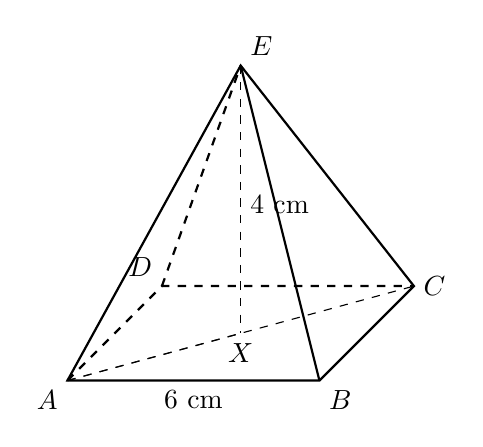
\begin{tikzpicture}[scale=0.8]
\coordinate (A) at (0,0);
\coordinate (B) at (4,0);
\coordinate (C) at (5.5,1.5);
\coordinate (D) at (1.5,1.5);
\coordinate (X) at (2.75,0.75);
\coordinate (E) at (2.75,5);
\draw[thick] (A) -- (B) -- (C) -- (E) -- cycle;
\draw[thick] (B) -- (E);
\draw[dashed, thick] (A) -- (D) -- (C);
\draw[dashed, thick] (D) -- (E);
\draw[dashed] (A) -- (C);
\draw[dashed] (E) -- (X);
\draw[dashed] (A) -- (X);
\node[below left] at (A) {$A$};
\node[below right] at (B) {$B$};
\node[right] at (C) {$C$};
\node[above left] at (D) {$D$};
\node[above right] at (E) {$E$};
\node[below] at (X) {$X$};
\node[below] at (2,0) {6 cm};
\node[right] at (2.75,2.8) {4 cm};
\end{tikzpicture}
\end{center}
\begin{enumerate}[label=\textbf{(\alph*)}, leftmargin=*]
\item Calculate the exact length of $AC$.
\examanswerslot{2cm}{0.25}{2}
\item Calculate the exact length of $AX$.
\examanswerslot{2cm}{0.25}{1}
\item Show that the length of the edge $AE$ is exactly $\sqrt{34}$ cm.
\examanswerslot{3.5cm}{0}{2}
\end{enumerate}
\vspace{1cm}\par\noindent\rule{\linewidth}{0.4pt}\vspace{1cm}
\item \needspace{5cm}
The diagram shows a cuboid with rectangular base $ABCD$ and top $EFGH$. \\
$AE$, $BF$, $CG$ and $DH$ are vertical edges. \\
$AB = 4$ cm, $BC = 3$ cm and $CG = 12$ cm. \\
\begin{center}
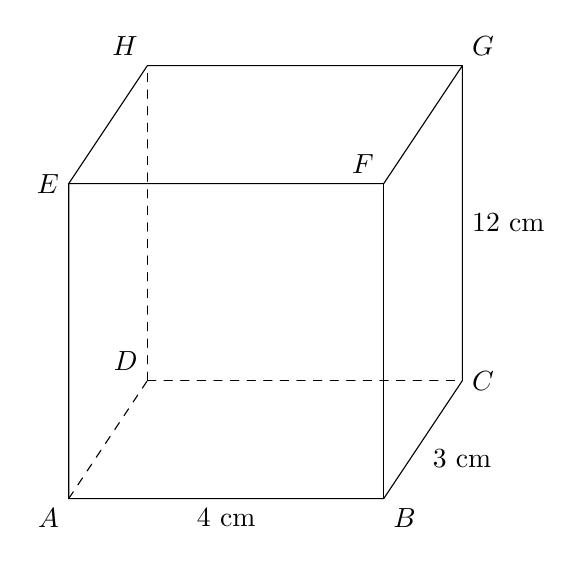
\begin{tikzpicture}[scale=1, line join=round, line cap=round]
\coordinate (A) at (0,0);
\coordinate (B) at (4,0);
\coordinate (C) at (5,1.5);
\coordinate (D) at (1,1.5);
\coordinate (E) at (0,4);
\coordinate (F) at (4,4);
\coordinate (G) at (5,5.5);
\coordinate (H) at (1,5.5);
\draw[dashed] (A) -- (D);
\draw[dashed] (D) -- (C);
\draw[dashed] (D) -- (H);
\draw (A) -- (B) -- (C) -- (G) -- (F) -- (E) -- cycle;
\draw (B) -- (F);
\draw (E) -- (H) -- (G);
\node[below left] at (A) {$A$};
\node[below right] at (B) {$B$};
\node[right] at (C) {$C$};
\node[above left] at (D) {$D$};
\node[left] at (E) {$E$};
\node[above left] at (F) {$F$};
\node[above right] at (G) {$G$};
\node[above left] at (H) {$H$};
\node[below] at (2,0) {$4$ cm};
\node[below right] at (4.5,0.75) {$3$ cm};
\node[right] at (5,3.5) {$12$ cm};
\end{tikzpicture}
\end{center}
\begin{enumerate}[label=\textbf{(\alph*)}, leftmargin=*]
\item Calculate the length $AC$.
\examanswerslot{2cm}{0.25}{2}
\item Calculate the length $AG$.
\examanswerslot{2cm}{0.25}{2}
\item Show that the sine of the angle between the line $AG$ and the plane $ABCD$ is
\par\vspace{0.1cm}\hspace*{0.6cm}$\dfrac{12}{13}$\par\vspace{0.15cm}
\examanswerslot{3.5cm}{0}{2}
\end{enumerate}
\vspace{1cm}\par\noindent\rule{\linewidth}{0.4pt}\vspace{1cm}
\item \needspace{5cm}
The diagram shows a pyramid with a square base $PQRS$. \\
The apex $V$ is directly above the centre $M$ of the base. \\
The sides of the square base are $6$ cm and the vertical height $VM$ is $3\sqrt{2}$ cm. \\
\begin{center}
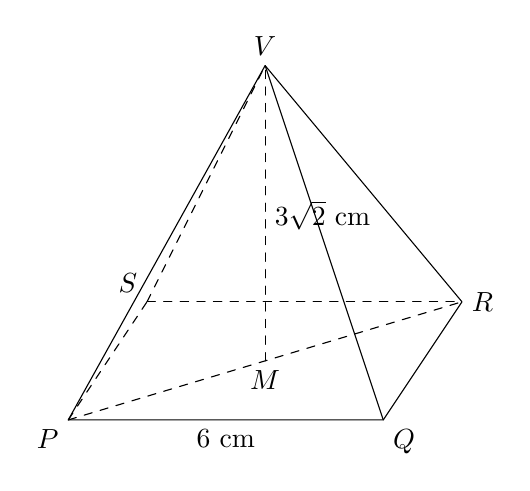
\begin{tikzpicture}[scale=1, line join=round, line cap=round]
\coordinate (P) at (0,0);
\coordinate (Q) at (4,0);
\coordinate (R) at (5,1.5);
\coordinate (S) at (1,1.5);
\coordinate (M) at (2.5,0.75);
\coordinate (V) at (2.5,4.5);
\draw[dashed] (P) -- (S);
\draw[dashed] (S) -- (R);
\draw[dashed] (S) -- (V);
\draw[dashed] (P) -- (R);
\draw[dashed] (M) -- (V);
\draw (P) -- (Q) -- (R) -- (V) -- cycle;
\draw (Q) -- (V);
\node[below left] at (P) {$P$};
\node[below right] at (Q) {$Q$};
\node[right] at (R) {$R$};
\node[above left] at (S) {$S$};
\node[below] at (M) {$M$};
\node[above] at (V) {$V$};
\node[below] at (2,0) {$6$ cm};
\node[right] at (2.5,2.6) {$3\sqrt{2}$ cm};
\end{tikzpicture}
\end{center}
\begin{enumerate}[label=\textbf{(\alph*)}, leftmargin=*]
\item Calculate the length $PR$.
\examanswerslot{2cm}{0.25}{2}
\item Calculate the length $PM$.
\examanswerslot{2cm}{0.25}{1}
\item Calculate the angle between the line $VP$ and the plane $PQRS$.
\examanswerslot{2cm}{0.25}{2}
\end{enumerate}
\vspace{1cm}\par\noindent\rule{\linewidth}{0.4pt}\vspace{1cm}
\item \needspace{5cm}
The diagram shows a cube with base $ABCD$ and top $EFGH$. \\
The side length of the cube is $2$ cm. \\
\begin{center}
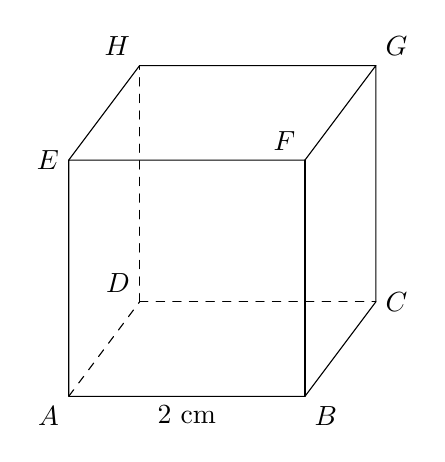
\begin{tikzpicture}[scale=1.5, line join=round, line cap=round]
\coordinate (A) at (0,0);
\coordinate (B) at (2,0);
\coordinate (C) at (2.6,0.8);
\coordinate (D) at (0.6,0.8);
\coordinate (E) at (0,2);
\coordinate (F) at (2,2);
\coordinate (G) at (2.6,2.8);
\coordinate (H) at (0.6,2.8);
\draw[dashed] (A) -- (D);
\draw[dashed] (D) -- (C);
\draw[dashed] (D) -- (H);
\draw (A) -- (B) -- (C) -- (G) -- (F) -- (E) -- cycle;
\draw (B) -- (F);
\draw (E) -- (H) -- (G);
\node[below left] at (A) {$A$};
\node[below right] at (B) {$B$};
\node[right] at (C) {$C$};
\node[above left] at (D) {$D$};
\node[left] at (E) {$E$};
\node[above left] at (F) {$F$};
\node[above right] at (G) {$G$};
\node[above left] at (H) {$H$};
\node[below] at (1,0) {$2$ cm};
\end{tikzpicture}
\end{center}
\begin{enumerate}[label=\textbf{(\alph*)}, leftmargin=*]
\item Calculate the length $FH$.
\examanswerslot{2cm}{0.25}{2}
\item Calculate the length $DF$.
\examanswerslot{2cm}{0.25}{2}
\item Show that the cosine of the angle between the line $DF$ and the plane $EFGH$ is
\par\vspace{0.1cm}\hspace*{0.6cm}$\sqrt{\dfrac{2}{3}}$\par\vspace{0.15cm}
\examanswerslot{3.5cm}{0}{2}
\end{enumerate}
\vspace{1cm}\par\noindent\rule{\linewidth}{0.4pt}\vspace{1cm}
\item \needspace{5cm}
The diagram shows a right triangular prism. \\
The base $ABED$ is a rectangle. \\
The triangles $ABC$ and $DEF$ are right-angled at $B$ and $E$. \\
$C$ is vertically above $B$ and $F$ is vertically above $E$. \\
$AB = 5$ cm, $BC = 5$ cm and $AD = 5\sqrt{2}$ cm. \\
\begin{center}
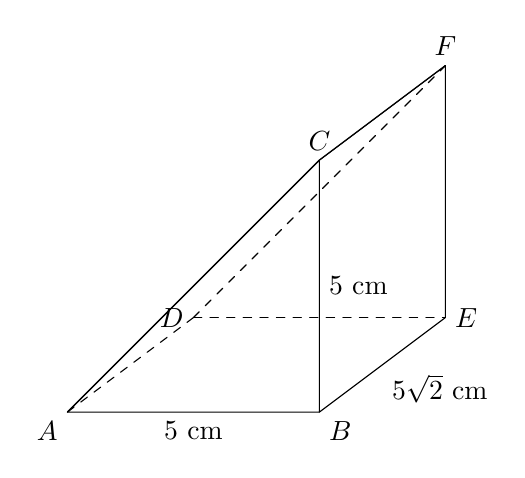
\begin{tikzpicture}[scale=0.8, line join=round, line cap=round]
\coordinate (A) at (0,0);
\coordinate (B) at (4,0);
\coordinate (C) at (4,4);
\coordinate (D) at (2,1.5);
\coordinate (E) at (6,1.5);
\coordinate (F) at (6,5.5);
\draw[dashed] (A) -- (D);
\draw[dashed] (D) -- (E);
\draw[dashed] (D) -- (F);
\draw (A) -- (B) -- (C) -- cycle;
\draw (B) -- (E) -- (F) -- (C);
\draw (A) -- (C) -- (F);
\node[below left] at (A) {$A$};
\node[below right] at (B) {$B$};
\node[above] at (C) {$C$};
\node[left] at (D) {$D$};
\node[right] at (E) {$E$};
\node[above] at (F) {$F$};
\node[below] at (2,0) {$5$ cm};
\node[below right] at (5,0.75) {$5\sqrt{2}$ cm};
\node[right] at (4,2) {$5$ cm};
\end{tikzpicture}
\end{center}
\begin{enumerate}[label=\textbf{(\alph*)}, leftmargin=*]
\item Calculate the length $BD$.
\examanswerslot{2cm}{0.25}{2}
\item Calculate the length $CD$.
\examanswerslot{2cm}{0.25}{2}
\item Calculate the angle between the line $CD$ and the plane $ABED$.
\examanswerslot{2cm}{0.25}{2}
\end{enumerate}
\vspace{1cm}\par\noindent\rule{\linewidth}{0.4pt}\vspace{1cm}
\item \needspace{5cm}
The diagram shows a pyramid with a rectangular base $WXYZ$. \\
The apex $V$ is directly above the centre $M$ of the base. \\
$WX = 8$ cm, $XY = 6$ cm and the vertical height $VM = 5\sqrt{3}$ cm. \\
\begin{center}
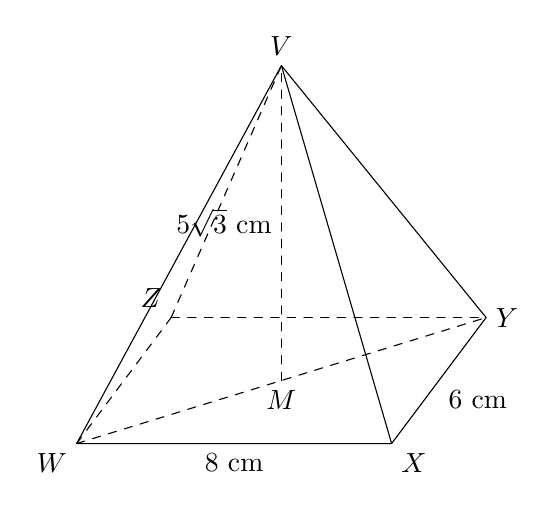
\begin{tikzpicture}[scale=0.8, line join=round, line cap=round]
\coordinate (W) at (0,0);
\coordinate (X) at (5,0);
\coordinate (Y) at (6.5,2);
\coordinate (Z) at (1.5,2);
\coordinate (M) at (3.25,1);
\coordinate (V) at (3.25,6);
\draw[dashed] (W) -- (Z);
\draw[dashed] (Z) -- (Y);
\draw[dashed] (Z) -- (V);
\draw[dashed] (W) -- (Y);
\draw[dashed] (M) -- (V);
\draw (W) -- (X) -- (Y) -- (V) -- cycle;
\draw (X) -- (V);
\node[below left] at (W) {$W$};
\node[below right] at (X) {$X$};
\node[right] at (Y) {$Y$};
\node[above left] at (Z) {$Z$};
\node[below] at (M) {$M$};
\node[above] at (V) {$V$};
\node[below] at (2.5,0) {$8$ cm};
\node[below right] at (5.75,1) {$6$ cm};
\node[left] at (3.25,3.5) {$5\sqrt{3}$ cm};
\end{tikzpicture}
\end{center}
\begin{enumerate}[label=\textbf{(\alph*)}, leftmargin=*]
\item Calculate the length $WY$.
\examanswerslot{2cm}{0.25}{2}
\item Calculate the length $MY$.
\examanswerslot{2cm}{0.25}{1}
\item Calculate the angle between the line $VY$ and the plane $WXYZ$.
\examanswerslot{2cm}{0.25}{2}
\end{enumerate}
\vspace{1cm}\par\noindent\rule{\linewidth}{0.4pt}\vspace{1cm}
\item \needspace{5cm}
The diagram shows a right pyramid $VABCD$ with a rectangular base $ABCD$. \\
$M$ is the centre of the base $ABCD$. \\
$AB = 8$ cm, $BC = 6$ cm and the vertical height $VM = 12$ cm. \\
\begin{center}
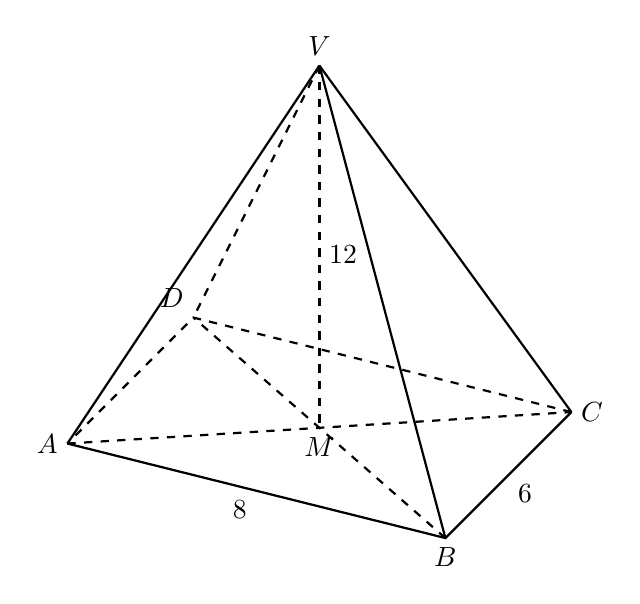
\begin{tikzpicture}[scale=0.8]
\coordinate (A) at (0,0);
\coordinate (B) at (6,-1.5);
\coordinate (C) at (8,0.5);
\coordinate (D) at (2,2);
\coordinate (M) at (4,0.25);
\coordinate (V) at (4,6);
\draw[thick] (A) -- (B) -- (C);
\draw[thick, dashed] (C) -- (D) -- (A);
\draw[thick] (V) -- (A);
\draw[thick] (V) -- (B);
\draw[thick] (V) -- (C);
\draw[thick, dashed] (V) -- (D);
\draw[thick, dashed] (A) -- (C);
\draw[thick, dashed] (B) -- (D);
\draw[thick, dashed] (V) -- (M);
\node[left] at (A) {$A$};
\node[below] at (B) {$B$};
\node[right] at (C) {$C$};
\node[above left] at (D) {$D$};
\node[below] at (M) {$M$};
\node[above] at (V) {$V$};
\node[below left] at (3,-0.75) {$8$};
\node[below right] at (7,-0.5) {$6$};
\node[right] at (4,3) {$12$};
\end{tikzpicture}
\end{center}
\begin{enumerate}[label=\textbf{(\alph*)}, leftmargin=*]
\item Calculate the length of $AM$.
\examanswerslot{2cm}{0.25}{2}
\item Calculate the length of $VA$.
\examanswerslot{2cm}{0.25}{2}
\item Show that the cosine of the angle between $VA$ and the plane $ABCD$ is $\dfrac{5}{13}$.
\examanswerslot{3.5cm}{0}{2}
\end{enumerate}
\vspace{1cm}\par\noindent\rule{\linewidth}{0.4pt}\vspace{1cm}
\item \needspace{5cm}
The diagram shows a cuboid $ABCDEFGH$. \\
\begin{center}
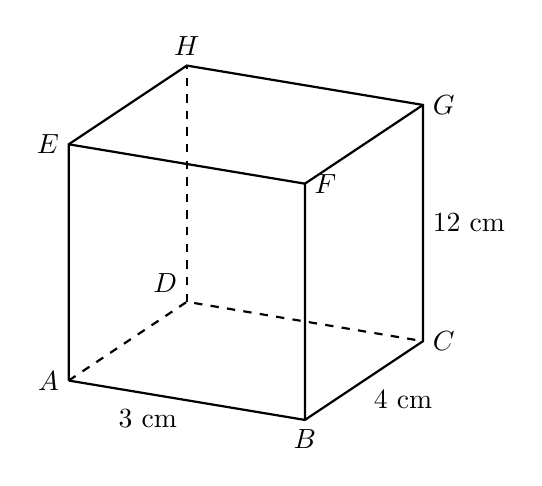
\begin{tikzpicture}[scale=1]
\coordinate (A) at (0,0);
\coordinate (B) at (3,-0.5);
\coordinate (C) at (4.5,0.5);
\coordinate (D) at (1.5,1);
\coordinate (E) at (0,3);
\coordinate (F) at (3,2.5);
\coordinate (G) at (4.5,3.5);
\coordinate (H) at (1.5,4);
\draw[thick] (A) -- (B) -- (C) -- (G) -- (H) -- (E) -- (A);
\draw[thick] (B) -- (F) -- (G);
\draw[thick] (E) -- (F);
\draw[thick, dashed] (A) -- (D) -- (C);
\draw[thick, dashed] (D) -- (H);
\node[left] at (A) {$A$};
\node[below] at (B) {$B$};
\node[right] at (C) {$C$};
\node[above left] at (D) {$D$};
\node[left] at (E) {$E$};
\node[right] at (F) {$F$};
\node[right] at (G) {$G$};
\node[above] at (H) {$H$};
\node[below left] at (1.5,-0.25) {$3$ cm};
\node[below right] at (3.75,0) {$4$ cm};
\node[right] at (4.5,2) {$12$ cm};
\end{tikzpicture}
\end{center}
$AB = 3$ cm, $BC = 4$ cm and $CG = 12$ cm. \\
\begin{enumerate}[label=\textbf{(\alph*)}, leftmargin=*]
\item Calculate the exact length of $AC$.
\examanswerslot{2cm}{0.25}{2}
\item Calculate the exact length of $AG$.
\examanswerslot{2cm}{0.25}{2}
\item Show that the sine of the angle between the line $AG$ and the plane $ABCD$ is given by the fraction:
\par\vspace{0.1cm}\hspace*{0.6cm}$\dfrac{12}{13}$\par\vspace{0.15cm}
\examanswerslot{3.5cm}{0}{2}
\end{enumerate}
\vspace{1cm}\par\noindent\rule{\linewidth}{0.4pt}\vspace{1cm}
\item \needspace{5cm}
The diagram shows a cube $ABCDEFGH$ with side length $x$ cm. \\
\begin{center}
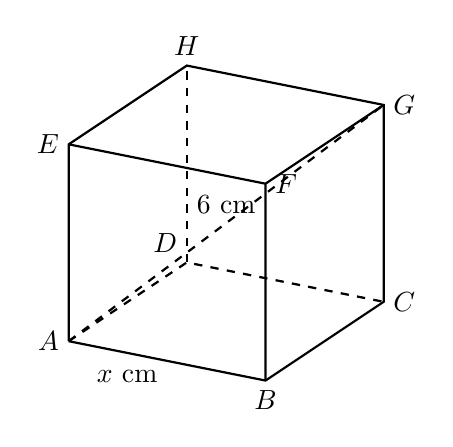
\begin{tikzpicture}[scale=1]
\coordinate (A) at (0,0);
\coordinate (B) at (2.5,-0.5);
\coordinate (C) at (4,0.5);
\coordinate (D) at (1.5,1);
\coordinate (E) at (0,2.5);
\coordinate (F) at (2.5,2);
\coordinate (G) at (4,3);
\coordinate (H) at (1.5,3.5);
\draw[thick] (A) -- (B) -- (C) -- (G) -- (H) -- (E) -- (A);
\draw[thick] (B) -- (F) -- (G);
\draw[thick] (E) -- (F);
\draw[thick, dashed] (A) -- (D) -- (C);
\draw[thick, dashed] (D) -- (H);
\draw[thick, dashed] (A) -- (G);
\node[left] at (A) {$A$};
\node[below] at (B) {$B$};
\node[right] at (C) {$C$};
\node[above left] at (D) {$D$};
\node[left] at (E) {$E$};
\node[right] at (F) {$F$};
\node[right] at (G) {$G$};
\node[above] at (H) {$H$};
\node[below left] at (1.25,-0.25) {$x$ cm};
\node[above, sloped] at (2,1.5) {$6$ cm};
\end{tikzpicture}
\end{center}
The internal diagonal $AG$ has a length of $6$ cm. \\
\noindent Write down an expression for $AC^2$ in terms of $x$. \par\vspace{0.1cm}
\examanswerslot{2cm}{0.25}{1}
\begin{enumerate}[label=\textbf{(\alph*)}, leftmargin=*]
\item Show that the exact value of $x$ is $2\sqrt{3}$.
\examanswerslot{3cm}{0}{2}
\item Find the exact value of the sine of the angle between the diagonal $AG$ and the plane $ABCD$.
\par\vspace{0.1cm}\hspace*{0.6cm}$\sin(\theta)$\par\vspace{0.15cm}
\examanswerslot{2.5cm}{0.25}{2}
\end{enumerate}
\vspace{1cm}\par\noindent\rule{\linewidth}{0.4pt}\vspace{1cm}
\item \needspace{5cm}
A right circular cone has vertex $P$ and the centre of its circular base is $O$. Points $A$ and $B$ lie on the circumference of the base such that $\angle AOB = 90^\circ$. The radius of the base is $6$ and the vertical height $PO$ is $8$. The point $M$ is the midpoint of the chord $AB$. \\
\begin{center}
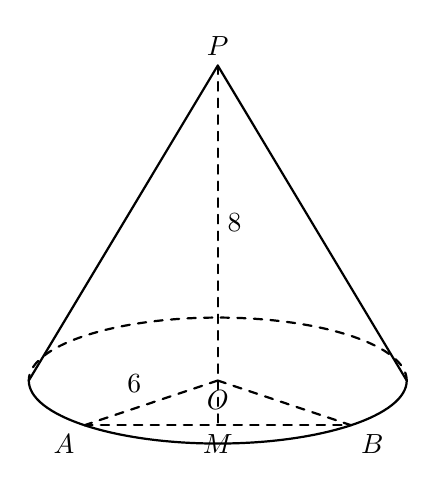
\begin{tikzpicture}[scale=0.8, line join=round, line cap=round]
\def\rx{3}
\def\ry{1}
\def\h{5}
\coordinate (O) at (0,0);
\coordinate (P) at (0,\h);
\draw[thick] (-\rx,0) arc (180:360:\rx cm and \ry cm);
\draw[thick, dashed] (\rx,0) arc (0:180:\rx cm and \ry cm);
\draw[thick] (-\rx,0) -- (P) -- (\rx,0);
\coordinate (A) at (-2.12,-0.71);
\coordinate (B) at (2.12,-0.71);
\coordinate (M) at (0,-0.71);
\draw[thick, dashed] (O)--(A);
\draw[thick, dashed] (O)--(B);
\draw[thick, dashed] (A)--(B);
\draw[thick, dashed] (P)--(O);
\draw[thick, dashed] (P)--(M);
\node[below] at (O) {$O$};
\node[above] at (P) {$P$};
\node[below left] at (A) {$A$};
\node[below right] at (B) {$B$};
\node[below] at (M) {$M$};
\node[above left] at (-1.06,-0.35) {$6$};
\node[right] at (0,2.5) {$8$};
\end{tikzpicture}
\end{center}
\begin{enumerate}[label=\textbf{(\alph*)}, leftmargin=*]
\item Calculate the exact length of the chord $AB$.
\examanswerslot{2cm}{0.25}{2}
\item Show that the length $OM$ is $3\sqrt{2}$.
\examanswerslot{3.5cm}{0}{2}
\item Find the exact value of $\tan(\angle PMO)$, which represents the true angle between the plane $PAB$ and the circular base.
\examanswerslot{2cm}{0.25}{2}
\end{enumerate}
\vspace{1cm}\par\noindent\rule{\linewidth}{0.4pt}\vspace{1cm}
\item \needspace{5cm}
A solid right prism has vertices $A, B, C, D, E, F$. The horizontal base $\triangle ABC$ is a right-angled triangle at $B$. The exact lengths are $AB = 8$, $BC = 6$, and the vertical height of the prism $AD = 24$. \\
\begin{center}
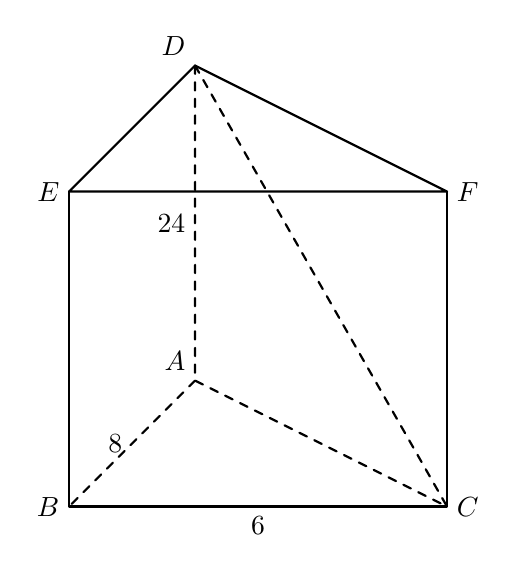
\begin{tikzpicture}[scale=0.8, line join=round, line cap=round]
\coordinate (A) at (0,0);
\coordinate (B) at (-2,-2);
\coordinate (C) at (4,-2);
\coordinate (D) at (0,5);
\coordinate (E) at (-2,3);
\coordinate (F) at (4,3);
\draw[thick] (D)--(E)--(F)--cycle;
\draw[thick] (E)--(B)--(C)--(F);
\draw[thick, dashed] (D)--(A)--(C);
\draw[thick, dashed] (A)--(B);
\draw[thick, dashed] (D)--(C);
\node[above left] at (D) {$D$};
\node[left] at (E) {$E$};
\node[right] at (F) {$F$};
\node[above left] at (A) {$A$};
\node[left] at (B) {$B$};
\node[right] at (C) {$C$};
\node[left] at (-1,-1) {$8$};
\node[below] at (1,-2) {$6$};
\node[left] at (0,2.5) {$24$};
\end{tikzpicture}
\end{center}
\begin{enumerate}[label=\textbf{(\alph*)}, leftmargin=*]
\item Calculate the length $AC$.
\examanswerslot{2cm}{0.25}{2}
\item Show that the length of the internal diagonal $DC$ is $26$.
\examanswerslot{3.5cm}{0}{2}
\item By calculating the exact square of the length $DB$, show that $\triangle DBC$ is right-angled at $B$.
\examanswerslot{3.5cm}{0}{3}
\item Find the exact value of $\cos(\angle DCB)$.
\examanswerslot{2cm}{0.25}{1}
\end{enumerate}
\vspace{1cm}\par\noindent\rule{\linewidth}{0.4pt}\vspace{1cm}
\item \needspace{5cm}
A local business analyses its daily advertising budget, $x$ GBP, and the corresponding daily revenue, $y$ GBP, over $8$ days. The data is documented in the table below. \\
\begin{center}
\renewcommand{\arraystretch}{1.5}
\begin{tabular}{|l|c|c|c|c|c|c|c|c|}
\hline
Advertising budget ($x$ GBP) & $10$ & $24$ & $35$ & $42$ & $58$ & $65$ & $74$ & $90$  \\
\hline
Daily revenue ($y$ GBP) & $90$ & $160$ & $205$ & $240$ & $310$ & $345$ & $380$ & $460$  \\
\hline
\end{tabular}
\end{center}
\begin{enumerate}[label=\textbf{(\alph*)}, leftmargin=*]
\item On the grid, complete the scatter diagram by plotting the remaining two points. The first six points have been plotted for you.
\begin{center}
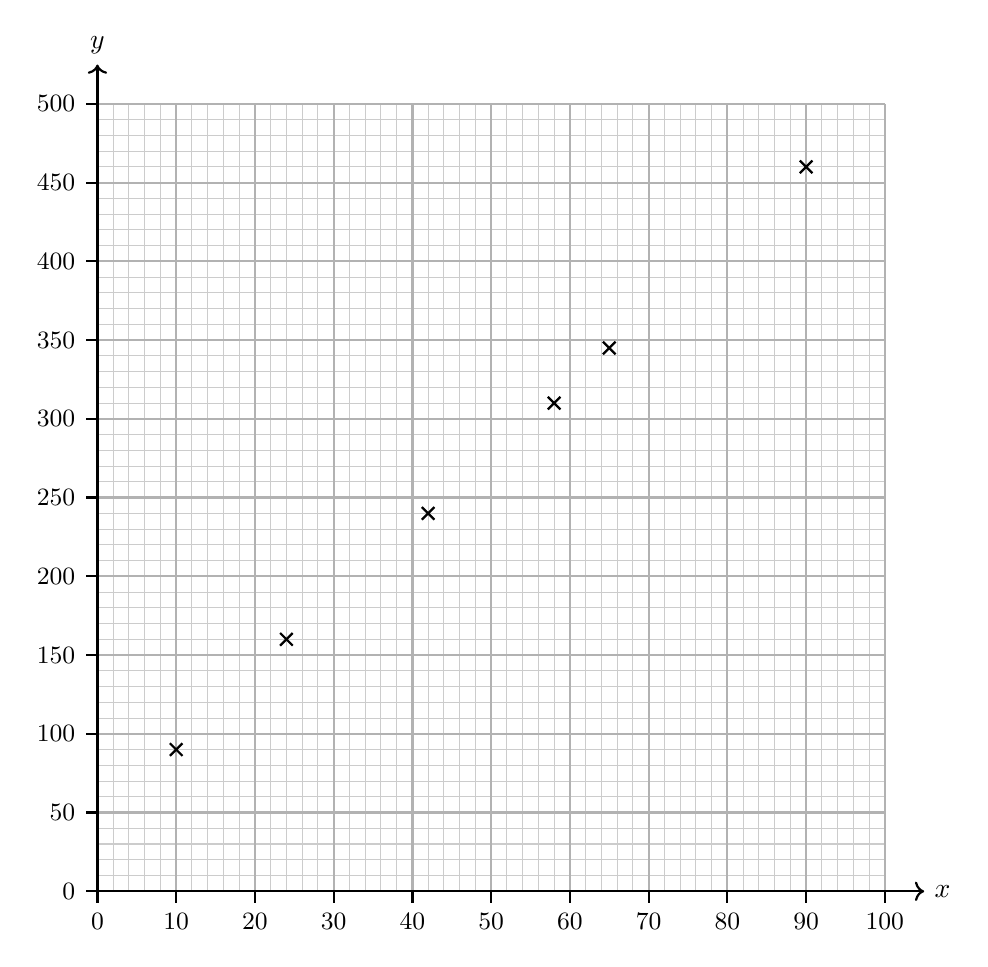
\begin{tikzpicture}
\draw[color=gray!40, xstep=0.2cm, ystep=0.2cm] (0,0) grid (10,10);
\draw[color=gray!60, thick, xstep=1cm, ystep=1cm] (0,0) grid (10,10);
\draw[thick, ->] (0,0) -- (10.5,0) node[right] {$x$};
\draw[thick, ->] (0,0) -- (0,10.5) node[above] {$y$};
\foreach \x [evaluate=\x as \val using int(\x*10)] in {0,1,2,3,4,5,6,7,8,9,10} {
\draw[thick] (\x,0) -- (\x,-0.15) node[below] {\small $\val$};
}
\foreach \y [evaluate=\y as \val using int(\y*50)] in {0,1,2,3,4,5,6,7,8,9,10} {
\draw[thick] (0,\y) -- (-0.15,\y) node[left] {\small $\val$};
}
\draw[thick] (1.0-0.08, 1.8-0.08) -- (1.0+0.08, 1.8+0.08);
\draw[thick] (1.0-0.08, 1.8+0.08) -- (1.0+0.08, 1.8-0.08);
\draw[thick] (2.4-0.08, 3.2-0.08) -- (2.4+0.08, 3.2+0.08);
\draw[thick] (2.4-0.08, 3.2+0.08) -- (2.4+0.08, 3.2-0.08);
\draw[thick] (4.2-0.08, 4.8-0.08) -- (4.2+0.08, 4.8+0.08);
\draw[thick] (4.2-0.08, 4.8+0.08) -- (4.2+0.08, 4.8-0.08);
\draw[thick] (5.8-0.08, 6.2-0.08) -- (5.8+0.08, 6.2+0.08);
\draw[thick] (5.8-0.08, 6.2+0.08) -- (5.8+0.08, 6.2-0.08);
\draw[thick] (6.5-0.08, 6.9-0.08) -- (6.5+0.08, 6.9+0.08);
\draw[thick] (6.5-0.08, 6.9+0.08) -- (6.5+0.08, 6.9-0.08);
\draw[thick] (9.0-0.08, 9.2-0.08) -- (9.0+0.08, 9.2+0.08);
\draw[thick] (9.0-0.08, 9.2+0.08) -- (9.0+0.08, 9.2-0.08);
\end{tikzpicture}
\end{center}
\phantom{.} \hfill \makebox[15pt][r]{[2]}
\item State the type of correlation shown in the scatter diagram.
\examanswerslot{1.5cm}{0.25}{1}
\item Use your graphic display calculator to find the equation of the linear regression line, giving your answer in the form $y = ax + b$.
\examanswerslot{2cm}{0.25}{2}
\item 
\begin{enumerate}[label=\textbf{(\roman*)}, leftmargin=0.6cm]
\item Use the regression equation to predict the daily revenue when the advertising budget is $120$ GBP.
\examanswerslot{2.5cm}{0.25}{2}
\item Explain why this prediction might not be reliable.
\examanswerslot{2cm}{0.25}{1}
\end{enumerate}
\end{enumerate}
\vspace{1cm}\par\noindent\rule{\linewidth}{0.4pt}\vspace{1cm}
\item \needspace{5cm}
An ice cream vendor records the midday temperature, $x$ in $^{\circ}\text{C}$, and their daily sales, $y$ in EUR, over a period of 8 days. The results are shown in the table. \\
\begin{center}
\begin{tabular}{|l|c|c|c|c|c|c|c|c|}
\hline
Temperature ($x$ $^{\circ}\text{C}$) & 12 & 14 & 16 & 18 & 22 & 24 & 26 & 28  \\
\hline
Sales ($y$ EUR) & 150 & 185 & 210 & 245 & 320 & 355 & 390 & 430  \\
\hline
\end{tabular}
\end{center}
\begin{enumerate}[label=\textbf{(\alph*)}, leftmargin=*]
\item Complete the scatter diagram by plotting the missing points for $x = 16$ and $x = 26$. Mark your points using small crosses ($\times$).
\begin{center}
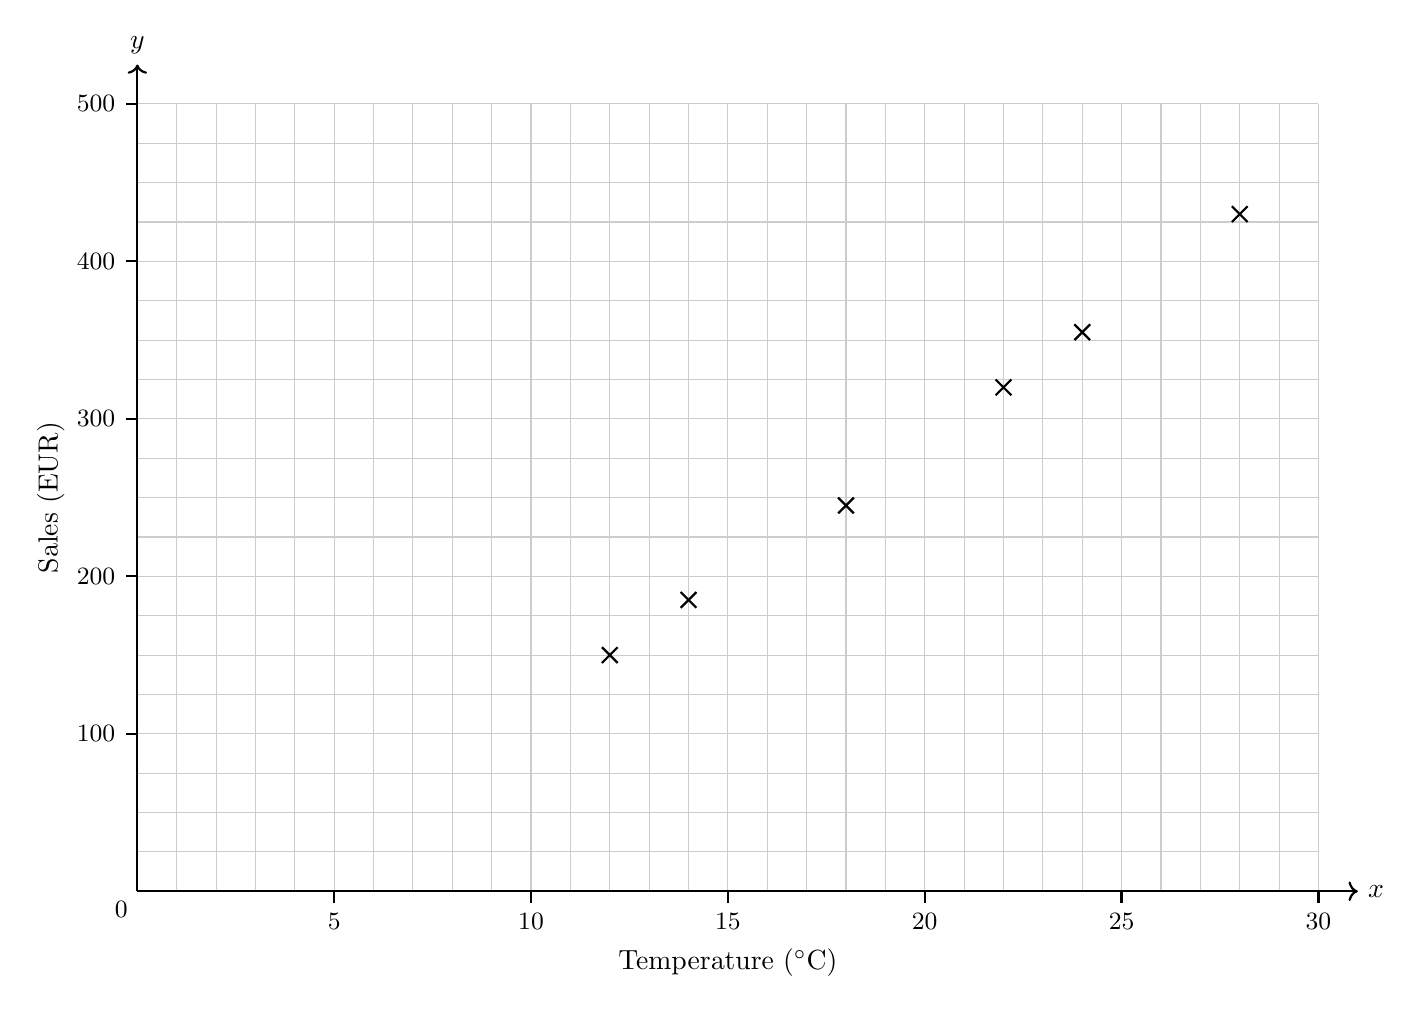
\begin{tikzpicture}
\draw[color=gray!40, xstep=0.5cm, ystep=0.5cm] (0,0) grid (15,10);
\draw[thick, ->] (0,0) -- (15.5,0) node[right] {$x$};
\draw[thick, ->] (0,0) -- (0,10.5) node[above] {$y$};
\node[below] at (7.5, -0.6) {Temperature ($^{\circ}\text{C}$)};
\node[rotate=90, above] at (-0.8, 5) {Sales (EUR)};
\foreach \x [evaluate=\x as \val using int(\x*2)] in {2.5,5.0,7.5,10.0,12.5,15.0} {
\draw[thick] (\x,0) -- (\x,-0.15) node[below] {\small $\val$};
}
\foreach \y [evaluate=\y as \val using int(\y*50)] in {2,4,6,8,10} {
\draw[thick] (0,\y) -- (-0.15,\y) node[left] {\small $\val$};
}
\node[below left] at (0,0) {\small $0$};
\draw[thick] (5.9, 2.9) -- (6.1, 3.1); \draw[thick] (5.9, 3.1) -- (6.1, 2.9);
\draw[thick] (6.9, 3.6) -- (7.1, 3.8); \draw[thick] (6.9, 3.8) -- (7.1, 3.6);
\draw[thick] (8.9, 4.8) -- (9.1, 5.0); \draw[thick] (8.9, 5.0) -- (9.1, 4.8);
\draw[thick] (10.9, 6.3) -- (11.1, 6.5); \draw[thick] (10.9, 6.5) -- (11.1, 6.3);
\draw[thick] (11.9, 7.0) -- (12.1, 7.2); \draw[thick] (11.9, 7.2) -- (12.1, 7.0);
\draw[thick] (13.9, 8.5) -- (14.1, 8.7); \draw[thick] (13.9, 8.7) -- (14.1, 8.5);
\end{tikzpicture}
\end{center}
\phantom{.} \hfill \makebox[15pt][r]{[2]}
\item State the type of correlation shown in the scatter diagram.
\examanswerslot{3cm}{0.25}{1}
\item Use your graphic display calculator to find the exact equation of the linear regression line in the form $y = mx + c$.
\examanswerslot{4cm}{0.25}{2}
\item Use your equation to estimate the sales on a day when the temperature is $20^{\circ}\text{C}$.
\examanswerslot{2cm}{0.25}{2}
\item Is your estimate in part (d) reliable? Give a reason for your answer.
\examanswerslot{5cm}{0.25}{1}
\end{enumerate}
\vspace{1cm}\par\noindent\rule{\linewidth}{0.4pt}\vspace{1cm}
\item \needspace{5cm}
The table shows the distance driven, $x$ km, and the amount of fuel remaining in the tank, $y$ litres, for a delivery van. \\
\begin{center}
\begin{tabular}{|l|c|c|c|c|c|c|c|c|}
\hline
Distance driven ($x$ km) & 20 & 50 & 80 & 110 & 140 & 170 & 200 & 230  \\
\hline
Fuel remaining ($y$ litres) & 45 & 42 & 38 & 35 & 32 & 29 & 25 & 22  \\
\hline
\end{tabular}
\end{center}
\begin{enumerate}[label=\textbf{(\alph*)}, leftmargin=*]
\item Plot the missing data points for $x = 80$ and $x = 200$ on the grid. Mark all points using small crosses ($\times$).
\begin{center}
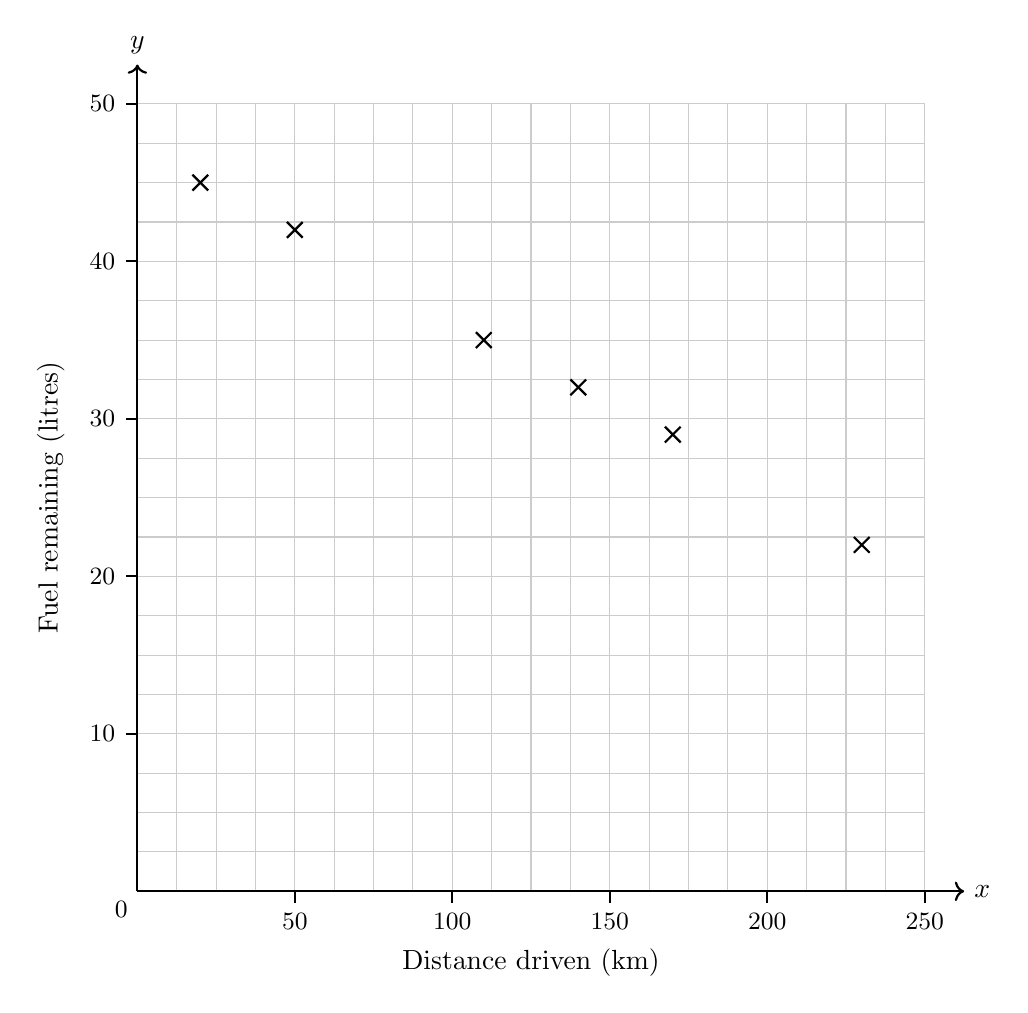
\begin{tikzpicture}
\draw[color=gray!40, xstep=0.5cm, ystep=0.5cm] (0,0) grid (10,10);
\draw[thick, ->] (0,0) -- (10.5,0) node[right] {$x$};
\draw[thick, ->] (0,0) -- (0,10.5) node[above] {$y$};
\node[below] at (5, -0.6) {Distance driven (km)};
\node[rotate=90, above] at (-0.8, 5) {Fuel remaining (litres)};
\foreach \x [evaluate=\x as \val using int(\x*25)] in {2,4,6,8,10} {
\draw[thick] (\x,0) -- (\x,-0.15) node[below] {\small $\val$};
}
\foreach \y [evaluate=\y as \val using int(\y*5)] in {2,4,6,8,10} {
\draw[thick] (0,\y) -- (-0.15,\y) node[left] {\small $\val$};
}
\node[below left] at (0,0) {\small $0$};
\draw[thick] (0.7, 8.9) -- (0.9, 9.1); \draw[thick] (0.7, 9.1) -- (0.9, 8.9);
\draw[thick] (1.9, 8.3) -- (2.1, 8.5); \draw[thick] (1.9, 8.5) -- (2.1, 8.3);
\draw[thick] (4.3, 6.9) -- (4.5, 7.1); \draw[thick] (4.3, 7.1) -- (4.5, 6.9);
\draw[thick] (5.5, 6.3) -- (5.7, 6.5); \draw[thick] (5.5, 6.5) -- (5.7, 6.3);
\draw[thick] (6.7, 5.7) -- (6.9, 5.9); \draw[thick] (6.7, 5.9) -- (6.9, 5.7);
\draw[thick] (9.1, 4.3) -- (9.3, 4.5); \draw[thick] (9.1, 4.5) -- (9.3, 4.3);
\end{tikzpicture}
\end{center}
\phantom{.} \hfill \makebox[15pt][r]{[2]}
\item Describe the correlation between distance driven and fuel remaining.
\examanswerslot{3cm}{0.25}{1} \vspace{1cm}
\item Use your graphic display calculator to find the exact equation of the linear regression line in the form $y = mx + c$. Give your parameters to $3$ significant figures.
\examanswerslot{4cm}{0.25}{2}
\item Predict the amount of fuel remaining after driving $300$ km.
\examanswerslot{2cm}{0.25}{2}
\item State whether the prediction in part (d) is an example of interpolation or extrapolation. Explain your reasoning.
\examanswerslot{5cm}{0.25}{1}
\end{enumerate}
\vspace{1cm}\par\noindent\rule{\linewidth}{0.4pt}\vspace{1cm}
\item \needspace{5cm}
A botanist tests a new fertilizer on 8 plants. The table records the mass of fertilizer applied, $x$ grams, and the resulting height of the plant, $y$ cm, after two months. \\
\begin{center}
\begin{tabular}{|l|c|c|c|c|c|c|c|c|}
\hline
Mass of fertilizer ($x$ g) & 5 & 10 & 15 & 20 & 25 & 30 & 35 & 40  \\
\hline
Height of plant ($y$ cm) & 12 & 15 & 19 & 24 & 28 & 33 & 36 & 41  \\
\hline
\end{tabular}
\end{center}
\begin{enumerate}[label=\textbf{(\alph*)}, leftmargin=*]
\item Two points are missing from the scatter diagram below. Plot the points corresponding to $x = 25$ and $x = 35$, marking them with small crosses ($\times$).
\begin{center}
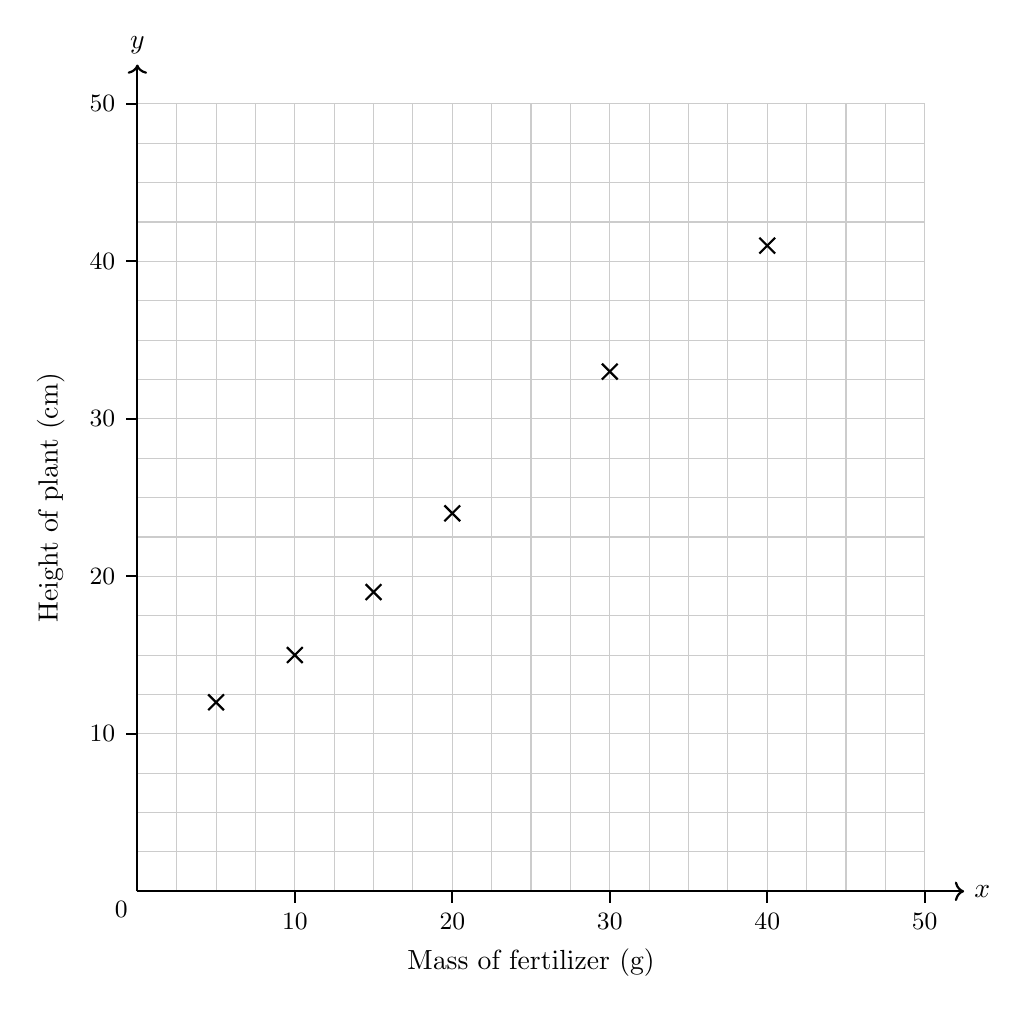
\begin{tikzpicture}
\draw[color=gray!40, xstep=0.5cm, ystep=0.5cm] (0,0) grid (10,10);
\draw[thick, ->] (0,0) -- (10.5,0) node[right] {$x$};
\draw[thick, ->] (0,0) -- (0,10.5) node[above] {$y$};
\node[below] at (5, -0.6) {Mass of fertilizer (g)};
\node[rotate=90, above] at (-0.8, 5) {Height of plant (cm)};
\foreach \x [evaluate=\x as \val using int(\x*5)] in {2,4,6,8,10} {
\draw[thick] (\x,0) -- (\x,-0.15) node[below] {\small $\val$};
}
\foreach \y [evaluate=\y as \val using int(\y*5)] in {2,4,6,8,10} {
\draw[thick] (0,\y) -- (-0.15,\y) node[left] {\small $\val$};
}
\node[below left] at (0,0) {\small $0$};
\draw[thick] (0.9, 2.3) -- (1.1, 2.5); \draw[thick] (0.9, 2.5) -- (1.1, 2.3);
\draw[thick] (1.9, 2.9) -- (2.1, 3.1); \draw[thick] (1.9, 3.1) -- (2.1, 2.9);
\draw[thick] (2.9, 3.7) -- (3.1, 3.9); \draw[thick] (2.9, 3.9) -- (3.1, 3.7);
\draw[thick] (3.9, 4.7) -- (4.1, 4.9); \draw[thick] (3.9, 4.9) -- (4.1, 4.7);
\draw[thick] (5.9, 6.5) -- (6.1, 6.7); \draw[thick] (5.9, 6.7) -- (6.1, 6.5);
\draw[thick] (7.9, 8.1) -- (8.1, 8.3); \draw[thick] (7.9, 8.3) -- (8.1, 8.1);
\end{tikzpicture}
\end{center}
\phantom{.} \hfill \makebox[15pt][r]{[2]}
\item State the correlation shown by your scatter graph.
\examanswerslot{3cm}{0.25}{1} \vspace{1cm}
\item Use your graphic display calculator to determine the equation of the line of best fit in the form $y = mx + c$.
\examanswerslot{4cm}{0.25}{2}
\item Using your equation, calculate the expected height of a plant that receives $18$ g of fertilizer.
\examanswerslot{2cm}{0.25}{2}
\item Give a reason why your prediction in part (d) is considered reliable.
\examanswerslot{4cm}{0.25}{1}
\end{enumerate}
\vspace{1cm}\par\noindent\rule{\linewidth}{0.4pt}\vspace{1cm}
\item \needspace{5cm}
A farmer records the mass of fertiliser applied ($x$ kg) and the corresponding yield of tomatoes ($y$ kg) from 8 identical plots of land. \\
\begin{center}
\begin{tabular}{|l|c|c|c|c|c|c|c|c|}
\hline
Mass of fertiliser ($x$ kg) & 2 & 3 & 5 & 6 & 8 & 9 & 11 & 12  \\
\hline
Yield of tomatoes ($y$ kg) & 14 & 19 & 27 & 32 & 41 & 45 & 52 & 58  \\
\hline
\end{tabular}
\end{center}
\begin{enumerate}[label=\textbf{(\alph*)}, leftmargin=*]
\item (a) Six of these points have been plotted on the scatter diagram below. Complete the diagram by plotting the remaining two points as small crosses ($\times$).
\begin{center}
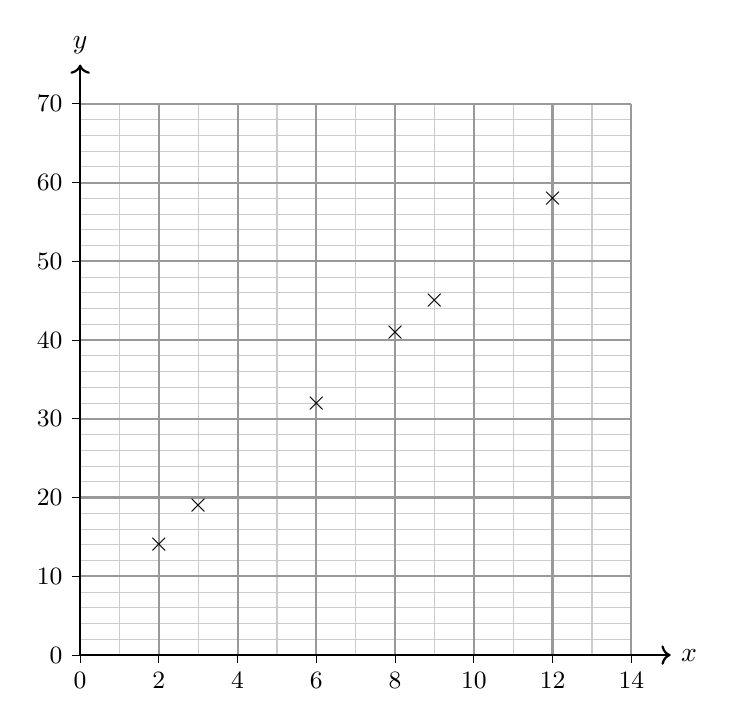
\begin{tikzpicture}
\draw[color=gray!40, xstep=0.5cm, ystep=0.2cm] (0,0) grid (7, 7);
\draw[thick, color=gray!80, step=1cm] (0,0) grid (7, 7);
\draw[thick, ->] (0,0) -- (7.5,0) node[right] {$x$};
\draw[thick, ->] (0,0) -- (0,7.5) node[above] {$y$};
\foreach \x/\val in {0/0, 1/2, 2/4, 3/6, 4/8, 5/10, 6/12, 7/14} {
\draw (\x,0) -- (\x,-0.1) node[below] {\small $\val$};
}
\foreach \y/\val in {0/0, 1/10, 2/20, 3/30, 4/40, 5/50, 6/60, 7/70} {
\draw (0,\y) -- (-0.1,\y) node[left] {\small $\val$};
}
\node at (1.0, 1.4) {$\times$};
\node at (1.5, 1.9) {$\times$};
\node at (3.0, 3.2) {$\times$};
\node at (4.0, 4.1) {$\times$};
\node at (4.5, 4.5) {$\times$};
\node at (6.0, 5.8) {$\times$};
\end{tikzpicture}
\end{center}
\phantom{.} \hfill \makebox[15pt][r]{[2]}
\item (b) Describe the correlation between the mass of fertiliser applied and the yield of tomatoes.
\examanswerslot{2cm}{0.25}{1}
\item (c) Utilise a graphic display calculator to determine the equation of the linear regression line, $y = mx + c$.
\examanswerslot{2cm}{0.25}{2} \vspace{1cm}
\item (d) Use your regression equation to estimate the yield of tomatoes when $10\text{ kg}$ of fertiliser is applied.
\examanswerslot{2cm}{0.25}{2}
\item (e) The farmer wants to use the equation to predict the yield if $16\text{ kg}$ of fertiliser is applied. Explain why this prediction might not be reliable.
\examanswerslot{2cm}{0.25}{1}
\end{enumerate}
\vspace{1cm}\par\noindent\rule{\linewidth}{0.4pt}\vspace{1cm}
\item \needspace{5cm}
A dealership analyses the relationship between the age of a specific car model in months, $x$, and its resale value in thousands of GBP, $y$. The data for 8 cars is given below. \\
\begin{center}
\begin{tabular}{|l|c|c|c|c|c|c|c|c|}
\hline
Age of car ($x$ months) & $0$ & $10$ & $25$ & $40$ & $50$ & $60$ & $75$ & $80$  \\
\hline
Resale value ($y$ thousand GBP) & $24$ & $21$ & $17$ & $12$ & $10$ & $8$ & $4$ & $2$  \\
\hline
\end{tabular}
\end{center}
\begin{enumerate}[label=\textbf{(\alph*)}, leftmargin=*]
\item Six points have already been plotted as small crosses ($\times$). Complete the scatter diagram by plotting the remaining two points as small crosses.
\begin{center}
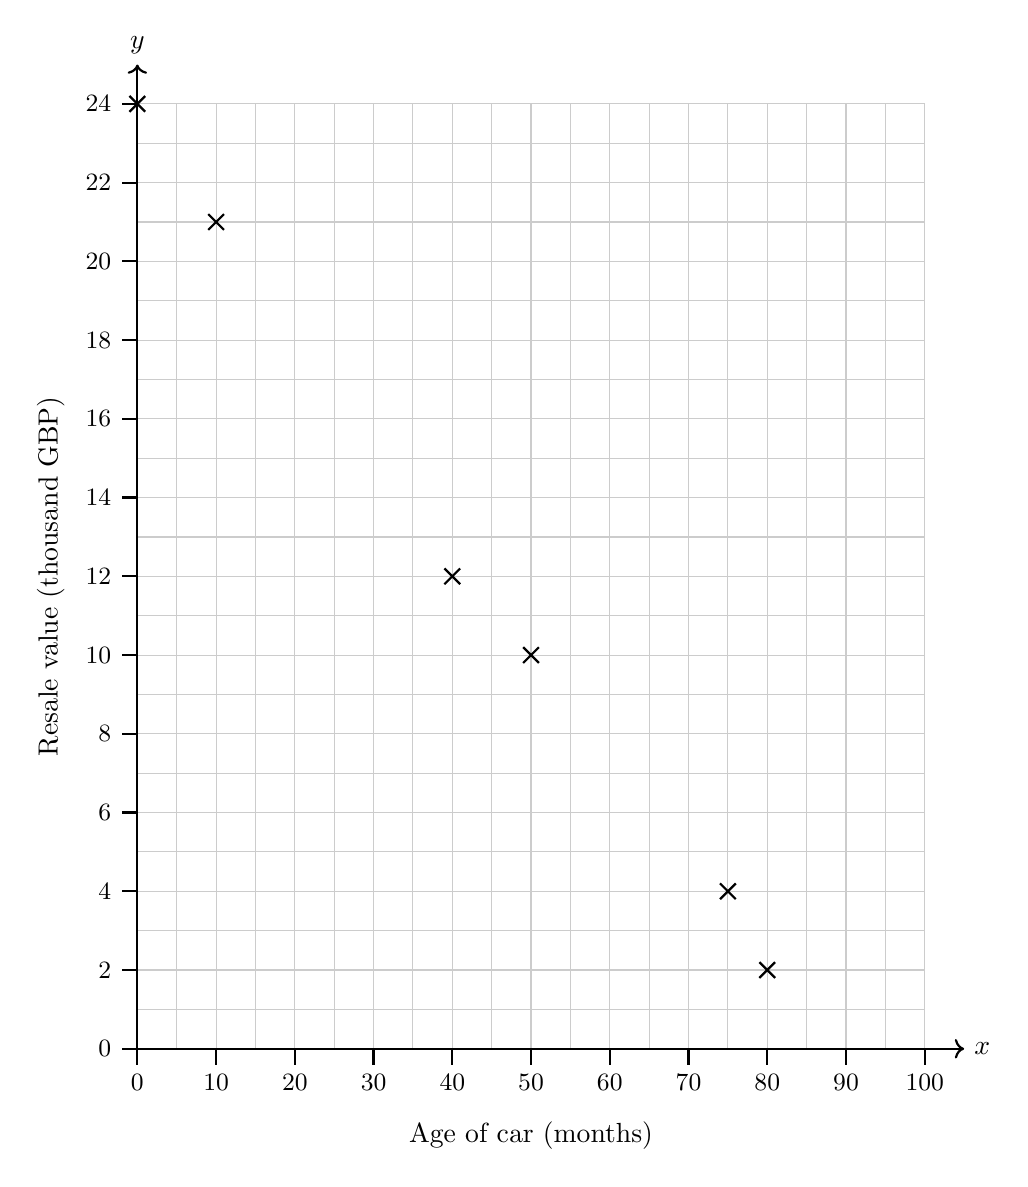
\begin{tikzpicture}
\draw[color=gray!40, xstep=0.5cm, ystep=0.5cm] (0,0) grid (10,12);
\draw[thick, ->] (0,0) -- (10.5,0) node[right] {$x$};
\draw[thick, ->] (0,0) -- (0,12.5) node[above] {$y$};
\foreach \x [evaluate=\x as \val using int(\x*10)] in {0,1,...,10} {
\draw[thick] (\x,0) -- (\x,-0.2) node[below] {\small $\val$};
}
\foreach \y [evaluate=\y as \val using int(\y*2)] in {0,1,...,12} {
\draw[thick] (0,\y) -- (-0.2,\y) node[left] {\small $\val$};
}
\foreach \px/\py in {0/12, 1/10.5, 4/6, 5/5, 7.5/2, 8/1} {
\draw[thick] (\px-0.1, \py-0.1) -- (\px+0.1, \py+0.1);
\draw[thick] (\px-0.1, \py+0.1) -- (\px+0.1, \py-0.1);
}
\node[below] at (5,-0.8) {Age of car (months)};
\node[rotate=90, above] at (-0.8,6) {Resale value (thousand GBP)};
\end{tikzpicture}
\end{center}
\phantom{.} \hfill \makebox[15pt][r]{[2]}
\item State the type of correlation shown in the scatter diagram.
\examanswerslot{2cm}{0.25}{1}
\item Find the exact equation of the linear regression line in the form $y = ax + b$. Give your parameters to 3 significant figures.
\examanswerslot{2cm}{0.25}{2}
\item Estimate the resale value of a car that is $35$ months old.
\examanswerslot{2cm}{0.25}{1}
\item Explain why it might not be sensible to use this regression equation to estimate the resale value of a car that is $120$ months old.
\examanswerslot{2cm}{0.25}{1}
\end{enumerate}
\vspace{1cm}\par\noindent\rule{\linewidth}{0.4pt}\vspace{1cm}
\item \needspace{5cm}
A researcher is investigating the relationship between the number of hours students spend studying independently over a month, $x$, and their final examination score, $y$. The data for 8 students is recorded in the table below. \\
\begin{center}
\begin{tabular}{|l|c|c|c|c|c|c|c|c|}
\hline
Study hours ($x$) & $4$ & $6$ & $9$ & $12$ & $14$ & $15$ & $18$ & $19$  \\
\hline
Exam score ($y$) & $35$ & $42$ & $58$ & $70$ & $76$ & $82$ & $90$ & $95$  \\
\hline
\end{tabular}
\end{center}
\begin{enumerate}[label=\textbf{(\alph*)}, leftmargin=*]
\item Some points have been plotted as small crosses ($\times$) on the grid for you. Complete the scatter diagram by plotting the remaining two points as small crosses.
\begin{center}
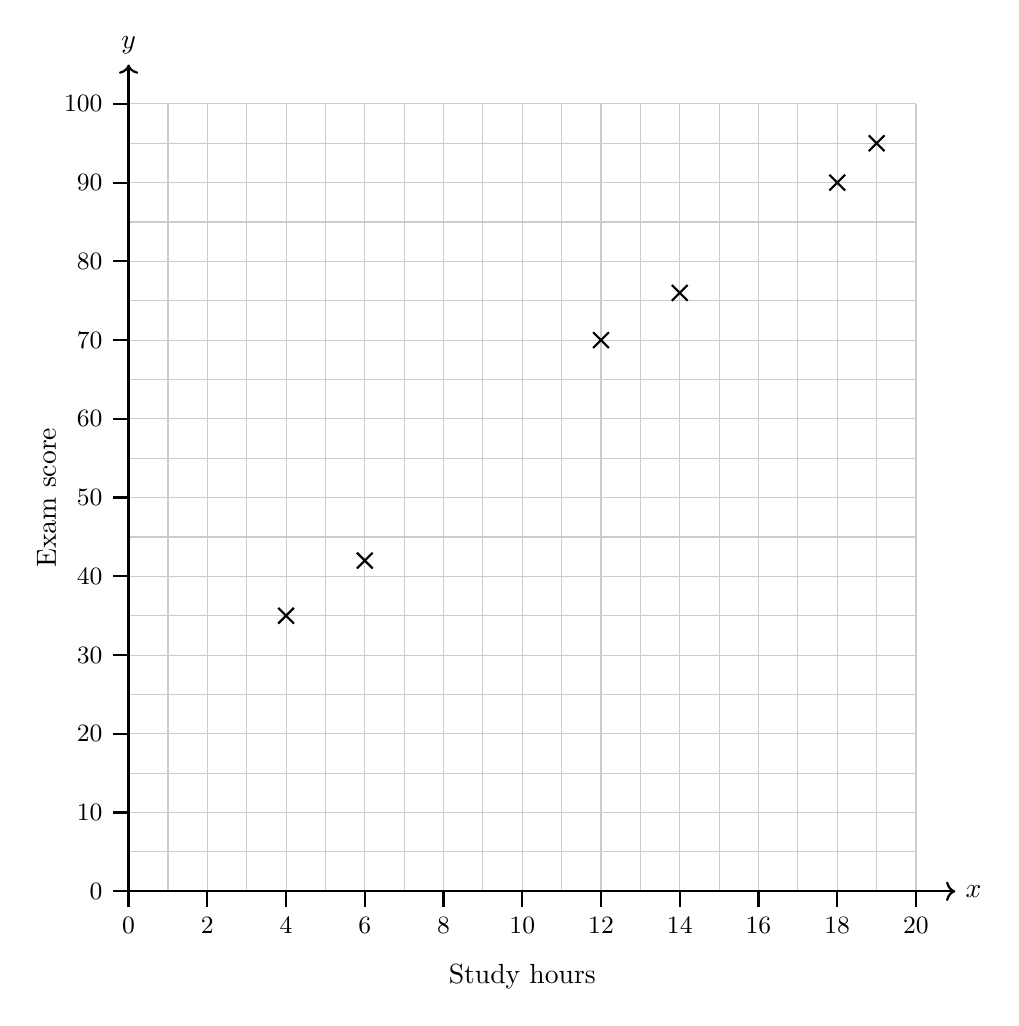
\begin{tikzpicture}
\draw[color=gray!40, xstep=0.5cm, ystep=0.5cm] (0,0) grid (10,10);
\draw[thick, ->] (0,0) -- (10.5,0) node[right] {$x$};
\draw[thick, ->] (0,0) -- (0,10.5) node[above] {$y$};
\foreach \x [evaluate=\x as \val using int(\x*2)] in {0,1,...,10} {
\draw[thick] (\x,0) -- (\x,-0.2) node[below] {\small $\val$};
}
\foreach \y [evaluate=\y as \val using int(\y*10)] in {0,1,...,10} {
\draw[thick] (0,\y) -- (-0.2,\y) node[left] {\small $\val$};
}
\foreach \px/\py in {2/3.5, 3/4.2, 6/7.0, 7/7.6, 9/9.0, 9.5/9.5} {
\draw[thick] (\px-0.1, \py-0.1) -- (\px+0.1, \py+0.1);
\draw[thick] (\px-0.1, \py+0.1) -- (\px+0.1, \py-0.1);
}
\node[below] at (5,-0.8) {Study hours};
\node[rotate=90, above] at (-0.8,5) {Exam score};
\end{tikzpicture}
\end{center}
\phantom{.} \hfill \makebox[15pt][r]{[2]}
\item What type of correlation does the scatter diagram show?
\examanswerslot{2cm}{0.25}{1} \vspace{1cm}
\item Use a graphic display calculator to find the exact equation of the linear regression line, giving your answer in the form $y = ax + b$. Give your values of $a$ and $b$ correct to 3 significant figures.
\examanswerslot{2cm}{0.25}{2}
\item Use your equation to estimate the exam score of a student who studied for $10$ hours.
\examanswerslot{2cm}{0.25}{1}
\item A student suggests using the regression line to predict the score of someone who studied for $30$ hours. State whether this prediction is valid and give a mathematical reason for your answer.
\examanswerslot{2cm}{0.25}{1}
\end{enumerate}
\vspace{1cm}\par\noindent\rule{\linewidth}{0.4pt}\vspace{1cm}
\item \needspace{5cm}
A student investigates the relationship between various pairs of variables. Four scatter diagrams, labelled A, B, C, and D, show different types of correlation. \\
\begin{center}
\begin{tikzpicture}[scale=0.7]
% Diagram A
\draw[thick, ->] (0,0) -- (4,0); \draw[thick, ->] (0,0) -- (0,4); \node at (2,-0.8) {A};
\foreach \x/\y in {0.5/1, 1/1.5, 1.5/1.2, 2/2.5, 2.5/2.2, 3/3.5, 3.5/3.1} { \node at (\x,\y) {$\times$}; }
% Diagram B
\begin{scope}[xshift=6cm]
\draw[thick, ->] (0,0) -- (4,0); \draw[thick, ->] (0,0) -- (0,4); \node at (2,-0.8) {B};
\foreach \x/\y in {0.5/3.5, 1/3.0, 1.5/3.2, 2/2.1, 2.5/1.8, 3/1.0, 3.5/0.8} { \node at (\x,\y) {$\times$}; }
\end{scope}
% Diagram C
\begin{scope}[yshift=-5.5cm]
\draw[thick, ->] (0,0) -- (4,0); \draw[thick, ->] (0,0) -- (0,4); \node at (2,-0.8) {C};
\foreach \x/\y in {0.5/2, 1/3.5, 1.5/1.2, 2/2.8, 2.5/0.8, 3/3.1, 3.5/1.9} { \node at (\x,\y) {$\times$}; }
\end{scope}
% Diagram D
\begin{scope}[xshift=6cm, yshift=-5.5cm]
\draw[thick, ->] (0,0) -- (4,0); \draw[thick, ->] (0,0) -- (0,4); \node at (2,-0.8) {D};
\foreach \x/\y in {0.5/0.5, 1/1.2, 1.5/2.5, 2/3.5, 2.5/2.8, 3/1.5, 3.5/0.8} { \node at (\x,\y) {$\times$}; }
\end{scope}
\end{tikzpicture}
\end{center}
\begin{enumerate}[label=\textbf{(\alph*)}, leftmargin=*]
\item State which diagram illustrates zero correlation.
\examanswerslot{2cm}{0.25}{1}
\item State which diagram illustrates a strong negative correlation.
\examanswerslot{2cm}{0.25}{1}
\item Describe the relationship between the variables plotted in Diagram A.
\examanswerslot{2cm}{0.25}{1}
\end{enumerate}
\vspace{1cm}\par\noindent\rule{\linewidth}{0.4pt}\vspace{1cm}
\item \begin{enumerate}[label=\textbf{(\alph*)}, leftmargin=*]
\item A large shipping container has a volume of $12\text{ m}^3$.
\begin{enumerate}[label=\textbf{(\roman*)}, leftmargin=0.6cm]
\item Convert this volume into cubic centimetres ($\text{cm}^3$).
\examanswerslot{2cm}{0.25}{1}
\item Convert this volume into litres.
\examanswerslot{2cm}{0.25}{1}
\end{enumerate}
\item A block of metal has a mass of $4.5\text{ kg}$. Convert this mass into grams ($\text{g}$).
\examanswerslot{2cm}{0.25}{1}
\end{enumerate}
\vspace{1cm}\par\noindent\rule{\linewidth}{0.4pt}\vspace{1cm}
\item \begin{enumerate}[label=\textbf{(\alph*)}, leftmargin=*]
\item A rectangular floor tile has an area of $600\text{ cm}^2$.
\begin{enumerate}[label=\textbf{(\roman*)}, leftmargin=0.6cm]
\item Convert this area into square millimetres ($\text{mm}^2$).
\examanswerslot{2cm}{0.25}{1}
\item Convert this area into square metres ($\text{m}^2$).
\examanswerslot{2cm}{0.25}{1}
\end{enumerate}
\item A bottle contains $350\text{ ml}$ of water. Convert this capacity into litres ($\text{l}$).
\examanswerslot{2cm}{0.25}{1}
\end{enumerate}
\vspace{1cm}\par\noindent\rule{\linewidth}{0.4pt}\vspace{1cm}
\item \begin{enumerate}[label=\textbf{(\alph*)}, leftmargin=*]
\item A field has an area of $0.05\text{ km}^2$.
\begin{enumerate}[label=\textbf{(\roman*)}, leftmargin=0.6cm]
\item Convert this area into square metres ($\text{m}^2$).
\examanswerslot{2cm}{0.25}{1}
\item Convert $150\text{ mm}^2$ into square centimetres ($\text{cm}^2$).
\examanswerslot{2cm}{0.25}{1}
\end{enumerate}
\item A storage box has a volume of $80\,000\text{ cm}^3$. Convert this volume into cubic metres ($\text{m}^3$).
\examanswerslot{2cm}{0.25}{1}
\end{enumerate}
\vspace{1cm}\par\noindent\rule{\linewidth}{0.4pt}\vspace{1cm}
\item \begin{enumerate}[label=\textbf{(\alph*)}, leftmargin=*]
\item A structural beam has a length of $2.8\text{ m}$.
\begin{enumerate}[label=\textbf{(\roman*)}, leftmargin=0.6cm]
\item Convert this length into millimetres ($\text{mm}$).
\examanswerslot{2cm}{0.25}{1}
\item Convert $250\text{ g}$ of flour into kilograms ($\text{kg}$).
\examanswerslot{2cm}{0.25}{1}
\end{enumerate}
\item A glass contains $0.45\text{ l}$ of juice. Convert this capacity into cubic centimetres ($\text{cm}^3$).
\examanswerslot{2cm}{0.25}{1}
\end{enumerate}
\vspace{1cm}\par\noindent\rule{\linewidth}{0.4pt}\vspace{1cm}
\item \noindent A solid gold statue has a volume of $350\text{ cm}^3$. \par\vspace{0.1cm}
\begin{enumerate}[label=\textbf{(\alph*)}, leftmargin=*]
\item Convert the volume of the statue into cubic millimetres ($\text{mm}^3$).
\examanswerslot{2cm}{0.25}{1}
\item The density of gold is $19.3\text{ g/cm}^3$. Calculate the mass of the statue in kilograms.
\examanswerslot{2cm}{0.25}{2}
\item A replica of the statue is made from a polymer where every linear dimension is scaled down by a factor of $\dfrac{1}{5}$. Calculate the volume of the replica in $\text{cm}^3$.
\examanswerslot{2cm}{0.25}{2}
\end{enumerate}
\vspace{1cm}\par\noindent\rule{\linewidth}{0.4pt}\vspace{1cm}
\item \noindent A large cylindrical water tank has a cross-sectional area of $2.5\text{ m}^2$. Water is poured into the tank at a constant rate of $150\text{ ml}$ per second. \par\vspace{0.1cm}
\begin{enumerate}[label=\textbf{(\alph*)}, leftmargin=*]
\item Express the flow rate of the water in litres per minute.
\examanswerslot{2cm}{0.25}{2}
\item Show that the height of the water in the tank increases by $3.6\text{ mm}$ each hour.
\examanswerslot{3.5cm}{0}{3}
\end{enumerate}
\vspace{1cm}\par\noindent\rule{\linewidth}{0.4pt}\vspace{1cm}
\item \noindent A cubic container has a total capacity of $0.027\text{ m}^3$. \par\vspace{0.1cm}
\begin{enumerate}[label=\textbf{(\alph*)}, leftmargin=*]
\item Find the capacity of the container in litres.
\examanswerslot{2cm}{0.25}{1}
\item Find the length of one edge of the container, giving your answer in centimetres.
\examanswerslot{2cm}{0.25}{2}
\item The container is filled with oil. A small pipe drains the oil at a rate of $45\text{ ml}$ per second. Calculate the time, in minutes, required to completely empty the full container.
\examanswerslot{2cm}{0.25}{2}
\end{enumerate}
\vspace{1cm}\par\noindent\rule{\linewidth}{0.4pt}\vspace{1cm}
\item \noindent A square agricultural test plot has a side length of $0.04\text{ km}$. \par\vspace{0.1cm}
\begin{enumerate}[label=\textbf{(\alph*)}, leftmargin=*]
\item Convert the side length of the test plot into millimetres ($\text{mm}$). Give your answer in standard scientific notation $A \times 10^n$.
\examanswerslot{2cm}{0.25}{2}
\item Calculate the total area of the agricultural test plot in square metres ($\text{m}^2$).
\examanswerslot{2cm}{0.25}{2}
\item A liquid nutrient treatment is applied uniformly over the plot at a rate of $150\text{ ml}$ per square metre. Calculate the total volume of nutrient treatment used over the entire plot, giving your final answer in litres ($\text{l}$).
\examanswerslot{2cm}{0.25}{2}
\end{enumerate}
\vspace{1cm}\par\noindent\rule{\linewidth}{0.4pt}\vspace{1cm}
\item A hypothetical dataset maps the depth of an underwater probe, $x$ metres, against the received signal strength index, $y$ units. A line of best fit is calculated from this survey and given by the linear regression equation: \\
\par\vspace{0.1cm}\hspace*{0.6cm}$y = 92.5 - 0.38x$\par\vspace{0.15cm}
\begin{enumerate}[label=\textbf{(\alph*)}, leftmargin=*]
\item State the type of correlation that this equation implies between the depth of the probe and the received signal strength index.
\examanswerslot{2cm}{0.25}{1}
\item Use the equation to calculate the predicted signal strength index when the probe is at a depth of 45.0 metres.
\examanswerslot{2cm}{0.25}{1}
\item Find the predicted depth of the probe when the signal strength index drops to 64.0 units.
\examanswerslot{2cm}{0.25}{2}
\end{enumerate}
\vspace{1cm}\par\noindent\rule{\linewidth}{0.4pt}\vspace{1cm}
\item \needspace{5cm}
A dealership records the age of used vehicles, $x$ years, and their selling price, $y$ in HKD. \\
\begin{center}
\begin{tabular}{|l|c|c|c|c|c|c|}
\hline
Age ($x$) & 2.5 & 4.0 & 5.5 & 7.0 & 8.5 & 10.0  \\
\hline
Price ($y$) & 125000 & 102500 & 80000 & 62500 & 45000 & 25000  \\
\hline
\end{tabular}
\end{center}
\begin{enumerate}[label=\textbf{(\alph*)}, leftmargin=*]
\item Complete the scatter diagram by plotting the remaining two points.
\begin{center}
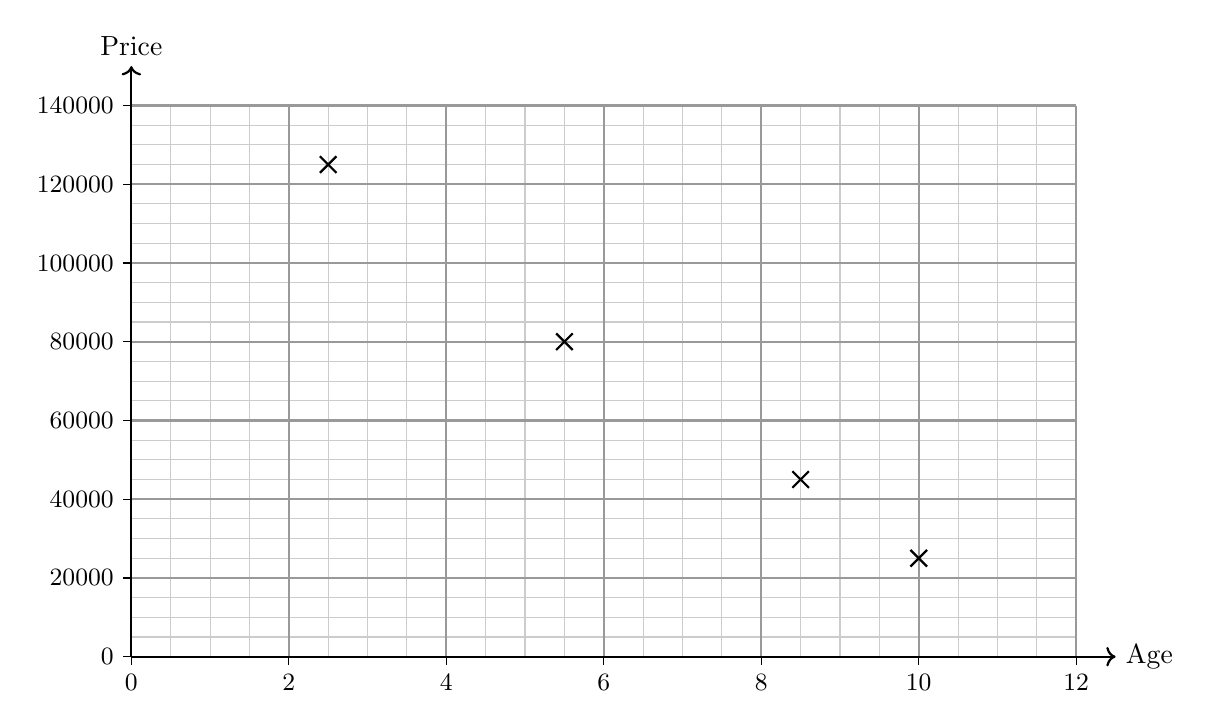
\begin{tikzpicture}
\draw[color=gray!40, xstep=0.5cm, ystep=0.25cm] (0,0) grid (12,7);
\draw[color=gray!80, thick, xstep=2cm, ystep=1cm] (0,0) grid (12,7);
\draw[thick, ->] (0,0) -- (12.5,0) node[right] {Age};
\draw[thick, ->] (0,0) -- (0,7.5) node[above] {Price};
\foreach \x/\val in {0/0, 2/2, 4/4, 6/6, 8/8, 10/10, 12/12} {
\draw (\x, 0) -- (\x, -0.1) node[below] {\small $\val$};
}
\foreach \y/\val in {0/0, 1/20000, 2/40000, 3/60000, 4/80000, 5/100000, 6/120000, 7/140000} {
\draw (0, \y) -- (-0.1, \y) node[left] {\small $\val$};
}
\draw[thick] (2.5cm - 3pt, 6.25cm - 3pt) -- (2.5cm + 3pt, 6.25cm + 3pt);
\draw[thick] (2.5cm - 3pt, 6.25cm + 3pt) -- (2.5cm + 3pt, 6.25cm - 3pt);
\draw[thick] (5.5cm - 3pt, 4.0cm - 3pt) -- (5.5cm + 3pt, 4.0cm + 3pt);
\draw[thick] (5.5cm - 3pt, 4.0cm + 3pt) -- (5.5cm + 3pt, 4.0cm - 3pt);
\draw[thick] (8.5cm - 3pt, 2.25cm - 3pt) -- (8.5cm + 3pt, 2.25cm + 3pt);
\draw[thick] (8.5cm - 3pt, 2.25cm + 3pt) -- (8.5cm + 3pt, 2.25cm - 3pt);
\draw[thick] (10.0cm - 3pt, 1.25cm - 3pt) -- (10.0cm + 3pt, 1.25cm + 3pt);
\draw[thick] (10.0cm - 3pt, 1.25cm + 3pt) -- (10.0cm + 3pt, 1.25cm - 3pt);
\end{tikzpicture}
\end{center}
\phantom{.} \hfill \makebox[15pt][r]{[2]}
\item State the type of correlation.
\examanswerslot{2cm}{0.25}{1}
\item Find the equation of the linear regression line in the form $y = mx + c$.
\examanswerslot{2.5cm}{0.25}{2}
\item Predict the selling price of a vehicle that is 6.5 years old.
\examanswerslot{2.5cm}{0.25}{2}
\end{enumerate}
\vspace{1cm}\par\noindent\rule{\linewidth}{0.4pt}\vspace{1cm}
\item A logistics company tracks the number of warehouse staff on duty, $x$, and the time taken to process a standard shipment, $y$ minutes. Data was collected for shifts where the number of staff members was strictly between 8 and 22. The linear regression equation for the time taken is calculated as: \\
\par\vspace{0.1cm}\hspace*{0.6cm}$y = 342.7 - 12.85x$\par\vspace{0.15cm}
\begin{enumerate}[label=\textbf{(\alph*)}, leftmargin=*]
\item State the type of correlation between the number of staff and the processing time.
\examanswerslot{2cm}{0.25}{1}
\item The mean number of staff on duty during the observed shifts is 16.
\begin{enumerate}[label=\textbf{(\roman*)}, leftmargin=0.6cm]
\item Calculate the mean time taken to process a standard shipment.
\examanswerslot{2cm}{0.25}{2}
\item Predict the processing time when 20 staff members are on duty.
\examanswerslot{2cm}{0.25}{2}
\end{enumerate}
\item A shipment is processed in 150 minutes. Estimate the number of staff on duty, giving your answer to the nearest whole number.
\examanswerslot{2.5cm}{0.25}{3}
\item State whether it is appropriate to use this equation to predict the processing time if 35 staff members are on duty. Give a clear reason for your answer.
\examanswerslot{2.5cm}{0.25}{1}
\end{enumerate}
\vspace{1cm}\par\noindent\rule{\linewidth}{0.4pt}\vspace{1cm}
\item A company purchases a piece of industrial machinery for 50000 EUR. The value of the machinery depreciates exponentially at a rate of 20\% each year. \\
\begin{enumerate}[label=\textbf{(\alph*)}, leftmargin=*]
\item Show that the value of the machinery after 2 years is 32000 EUR.
\examanswerslot{3.5cm}{0}{2}
\item Calculate the value of the machinery after 3 years.
\examanswerslot{2cm}{0.25}{2}
\end{enumerate}
\vspace{1cm}\par\noindent\rule{\linewidth}{0.4pt}\vspace{1cm}
\item The population of a small village is tracked using an exponential growth model. The initial population of the village is 1200. The population increases at a constant rate of 5\% each year. \\
\begin{enumerate}[label=\textbf{(\alph*)}, leftmargin=*]
\item Find the population of the village after 1 year.
\examanswerslot{2cm}{0.25}{1}
\item Calculate the population of the village after 2 years.
\examanswerslot{2cm}{0.25}{2}
\end{enumerate}
\vspace{1cm}\par\noindent\rule{\linewidth}{0.4pt}\vspace{1cm}
\item A delivery fleet vehicle was bought for 16000 AUD. The vehicle's value loses value exponentially at a rate of 50\% per year. \\
\begin{enumerate}[label=\textbf{(\alph*)}, leftmargin=*]
\item Calculate the value of the vehicle after 3 years.
\examanswerslot{2cm}{0.25}{2}
\item Determine the total value lost by the vehicle over these 3 years.
\examanswerslot{2cm}{0.25}{1}
\end{enumerate}
\vspace{1cm}\par\noindent\rule{\linewidth}{0.4pt}\vspace{1cm}
\item A herd of rare deer in a nature reserve has an initial population of 480. The population increases exponentially at a rate of 6.4\% per year. \\
\begin{enumerate}[label=\textbf{(\alph*)}, leftmargin=*]
\item Calculate the expected population of the herd after 5 years. Give your answer to the nearest whole number.
\examanswerslot{2cm}{0.25}{2}
\item Calculate the number of complete years it will take for the population of the herd to exceed 1000.
\examanswerslot{2cm}{0.25}{3}
\end{enumerate}
\vspace{1cm}\par\noindent\rule{\linewidth}{0.4pt}\vspace{1cm}
\item A manufacturing company purchases a heavy industrial machine for 75000 EUR. The value of the machine depreciates exponentially at a constant rate of 12.5\% per year. \\
\begin{enumerate}[label=\textbf{(\alph*)}, leftmargin=*]
\item Calculate the value of the machine after 4 years. Give your answer to the nearest EUR.
\examanswerslot{2cm}{0.25}{2}
\item Find the total percentage depreciation in the value of the machine over these 4 years.
\examanswerslot{2cm}{0.25}{2}
\end{enumerate}
\vspace{1cm}\par\noindent\rule{\linewidth}{0.4pt}\vspace{1cm}
\item An investor purchases a vintage car as an asset for 42000 AUD. The value of the asset increases exponentially at a fixed rate of 5.8\% per year. \\
\begin{enumerate}[label=\textbf{(\alph*)}, leftmargin=*]
\item Calculate the value of the vintage car after 6 years. Give your answer correct to the nearest 100 AUD.
\examanswerslot{2cm}{0.25}{2}
\item Calculate the number of complete years required for the original investment value to increase by at least 75\% .
\examanswerslot{2cm}{0.25}{3}
\end{enumerate}
\vspace{1cm}\par\noindent\rule{\linewidth}{0.4pt}\vspace{1cm}
\item A tech company tracks the active user base of a new digital platform. The initial group consists of 12500 active users and increases exponentially at a rate of 18.2\% per month. \\
\begin{enumerate}[label=\textbf{(\alph*)}, leftmargin=*]
\item Calculate the number of active users after 8 months. Give your answer correct to 3 significant figures.
\examanswerslot{2cm}{0.25}{2}
\item Find the number of complete months it takes for the user base to reach 5 times its initial size.
\examanswerslot{2cm}{0.25}{3}
\end{enumerate}
\vspace{1cm}\par\noindent\rule{\linewidth}{0.4pt}\vspace{1cm}
\item A regional wildlife reserve tracks the population of an endangered species of wetland birds. At the start of 2018, a comprehensive census records the population at 1420 birds. Due to habitat restoration and conservation efforts, the population increases at a continuous compound rate of 4.3\% per year. \\
\begin{enumerate}[label=\textbf{(\alph*)}, leftmargin=*]
\item Calculate the expected population of the wetland birds at the start of 2026. Give your answer to the nearest whole number.
\examanswerslot{2cm}{0.25}{2}
\item Find the number of complete years it will take for the initial population of 1420 birds to double.
\examanswerslot{2cm}{0.25}{3}
\end{enumerate}
\vspace{1cm}\par\noindent\rule{\linewidth}{0.4pt}\vspace{1cm}
\item A manufacturing logistics company purchases a fleet of heavy-duty delivery vehicles for a total initial asset value of 485000 EUR. The financial accounting team applies a reducing-balance depreciation model where the total value of the fleet decreases at a constant rate of 12.6\% per annum. \\
\begin{enumerate}[label=\textbf{(\alph*)}, leftmargin=*]
\item Calculate the value of the fleet of vehicles at the end of 6 years. Give your answer correct to 3 significant figures.
\examanswerslot{2cm}{0.25}{2}
\item Show that the value of the fleet decreases to less than half of its initial purchase value during the 6th year.
\examanswerslot{3.5cm}{0}{3}
\end{enumerate}
\vspace{1cm}\par\noindent\rule{\linewidth}{0.4pt}\vspace{1cm}
\item An marine biology study monitors the population of a specific invasive fish species in a closed bay ecosystem. Biologists estimate the population at 8500 fish at the beginning of a monitoring phase. Due to resources becoming scarce, the population decreases at a constant rate of 6.8\% each month. \\
\begin{enumerate}[label=\textbf{(\alph*)}, leftmargin=*]
\item Calculate the estimated population of the invasive fish species after 1.5 years. Give your answer to the nearest hundred fish.
\examanswerslot{2cm}{0.25}{3}
\item Determine the number of months required for the population to decrease from 8500 to below 2500 fish.
\examanswerslot{2cm}{0.25}{3}
\end{enumerate}
\vspace{1cm}\par\noindent\rule{\linewidth}{0.4pt}\vspace{1cm}
\item The population of Town A is currently 45000 and is decreasing at a rate of 1.8\% per year. \\
The population of Town B is currently 32000 and is increasing at a rate of 2.4\% per year. \\
\begin{enumerate}[label=\textbf{(\alph*)}, leftmargin=*]
\item Calculate the population of Town A after exactly 5 years, giving your answer correct to 3 significant figures.
\examanswerslot{2cm}{0.25}{2}
\item Show that after $n$ years, the condition for Town B's population to exceed Town A's population simplifies to the inequality:
\par\vspace{0.1cm}\hspace*{0.6cm}$\left(\dfrac{1.024}{0.982}\right)^n > \dfrac{45}{32}$\par\vspace{0.15cm}
\examanswerslot{3.5cm}{0}{2}
\item Hence calculate the minimum integer value of $n$ for which Town B has a greater population than Town A.
\examanswerslot{2cm}{0.25}{3}
\end{enumerate}
\vspace{1cm}\par\noindent\rule{\linewidth}{0.4pt}\vspace{1cm}
\item A manufacturing company purchases a specialized robotic machine for 125000 USD. \\
The machine depreciates in value by 15\% per year for the first 3 years. It then depreciates by $r\%$ per year for every subsequent year. \\
\begin{enumerate}[label=\textbf{(\alph*)}, leftmargin=*]
\item Calculate the value of the machine after exactly 3 years.
\examanswerslot{2cm}{0.25}{2}
\item After exactly 8 years, the total value of the machine is 41500 USD. Calculate the value of $r$, correct to 3 significant figures.
\examanswerslot{2cm}{0.25}{3}
\item A different robotic machine depreciates at a constant rate of 12\% per year. Its value today is 28160 USD. Calculate its original value exactly 6 years ago.
\examanswerslot{2cm}{0.25}{3}
\end{enumerate}
\vspace{1cm}\par\noindent\rule{\linewidth}{0.4pt}\vspace{1cm}
\item A nature reserve introduces a population of 850 deer. \\
The population increases by 8\% per year for the first 5 years. A specific disease then causes the population to decrease by $k\%$ per year subsequently. \\
\begin{enumerate}[label=\textbf{(\alph*)}, leftmargin=*]
\item Calculate the number of deer at the end of the first 5 years, giving your answer to the nearest whole number.
\examanswerslot{2cm}{0.25}{2}
\item Ten years after the initial introduction, the population has fallen to 720 deer. Calculate the value of $k$, correct to 3 significant figures.
\examanswerslot{2cm}{0.25}{3}
\item Assuming the disease continues at the exact same exponential rate, calculate the total number of years from the initial introduction until the population first drops below 500 deer.
\examanswerslot{2cm}{0.25}{4}
\end{enumerate}
\vspace{1cm}\par\noindent\rule{\linewidth}{0.4pt}\vspace{1cm}
\item A rare gemstone is bought for 15000 GBP. Its value increases exponentially at a constant percentage rate. After 4 years, its value is exactly 18500 GBP. \\
\begin{enumerate}[label=\textbf{(\alph*)}, leftmargin=*]
\item Calculate the annual percentage increase in the value of the gemstone, correct to 3 significant figures.
\examanswerslot{2cm}{0.25}{3}
\item A gold watch is bought at the same time for $V$ GBP. Its value decreases by 3.5\% per year. After exactly 7 years, the value of the gold watch is exactly half the value of the gemstone. Show that $V = 13900$ GBP, correct to 3 significant figures.
\examanswerslot{3.5cm}{0}{3}
\item Calculate the minimum number of whole years it takes from the time of purchase for the gemstone's value to be more than three times the gold watch's value.
\examanswerslot{2cm}{0.25}{4}
\end{enumerate}
\vspace{1cm}\par\noindent\rule{\linewidth}{0.4pt}\vspace{1cm}
\item \begin{enumerate}[label=\textbf{(\alph*)}, leftmargin=*]
\item Simplify completely.
\par\vspace{0.1cm}\hspace*{0.6cm}$ \sqrt{32} $\par\vspace{0.15cm}
\examanswerslot{2cm}{0.25}{1}
\item Rationalise the denominator and simplify.
\par\vspace{0.1cm}\hspace*{0.6cm}$ \dfrac{12}{\sqrt{6}} $\par\vspace{0.15cm}
\examanswerslot{2.5cm}{0.25}{2}
\end{enumerate}
\vspace{1cm}\par\noindent\rule{\linewidth}{0.4pt}\vspace{1cm}
\item \begin{enumerate}[label=\textbf{(\alph*)}, leftmargin=*]
\item Simplify the expression.
\par\vspace{0.1cm}\hspace*{0.6cm}$ \sqrt{75} + \sqrt{12} $\par\vspace{0.15cm}
\examanswerslot{3cm}{0.25}{2}
\item Rationalise the denominator.
\par\vspace{0.1cm}\hspace*{0.6cm}$ \dfrac{10}{\sqrt{5}} $\par\vspace{0.15cm}
\examanswerslot{2.5cm}{0.25}{2}
\end{enumerate}
\vspace{1cm}\par\noindent\rule{\linewidth}{0.4pt}\vspace{1cm}
\item \begin{enumerate}[label=\textbf{(\alph*)}, leftmargin=*]
\item Simplify.
\par\vspace{0.1cm}\hspace*{0.6cm}$ \sqrt{80} $\par\vspace{0.15cm}
\examanswerslot{2cm}{0.25}{1}
\item Show that the following expression simplifies to $5\sqrt{3}$.
\par\vspace{0.1cm}\hspace*{0.6cm}$ \dfrac{15}{\sqrt{3}} $\par\vspace{0.15cm}
\examanswerslot{3.5cm}{0}{2}
\end{enumerate}
\vspace{1cm}\par\noindent\rule{\linewidth}{0.4pt}\vspace{1cm}
\item \begin{enumerate}[label=\textbf{(\alph*)}, leftmargin=*]
\item Simplify.
\par\vspace{0.1cm}\hspace*{0.6cm}$ \sqrt{28} - \sqrt{7} $\par\vspace{0.15cm}
\examanswerslot{2.5cm}{0.25}{2}
\item Rationalise the denominator.
\par\vspace{0.1cm}\hspace*{0.6cm}$ \dfrac{8}{\sqrt{2}} $\par\vspace{0.15cm}
\examanswerslot{2.5cm}{0.25}{2}
\end{enumerate}
\vspace{1cm}\par\noindent\rule{\linewidth}{0.4pt}\vspace{1cm}
\item \begin{enumerate}[label=\textbf{(\alph*)}, leftmargin=*]
\item (a) Simplify fully.
\par\vspace{0.1cm}\hspace*{0.6cm}$ 3\sqrt{48} - \sqrt{12} $\par\vspace{0.15cm}
\examanswerslot{2.5cm}{0.25}{2}
\item (b) Rationalise the denominator and simplify fully.
\par\vspace{0.1cm}\hspace*{0.6cm}$ \dfrac{5 + \sqrt{3}}{2 + \sqrt{3}} $\par\vspace{0.15cm}
\examanswerslot{4cm}{0.25}{3}
\end{enumerate}
\vspace{1cm}\par\noindent\rule{\linewidth}{0.4pt}\vspace{1cm}
\item \begin{enumerate}[label=\textbf{(\alph*)}, leftmargin=*]
\item (a) Simplify fully.
\par\vspace{0.1cm}\hspace*{0.6cm}$ \sqrt{98} - \sqrt{50} $\par\vspace{0.15cm}
\examanswerslot{2.5cm}{0.25}{2}
\item (b) Rationalise the denominator.
\par\vspace{0.1cm}\hspace*{0.6cm}$ \dfrac{8}{3 + \sqrt{5}} $\par\vspace{0.15cm}
\examanswerslot{3.5cm}{0.25}{3}
\end{enumerate}
\vspace{1cm}\par\noindent\rule{\linewidth}{0.4pt}\vspace{1cm}
\item \begin{enumerate}[label=\textbf{(\alph*)}, leftmargin=*]
\item (a) Expand and simplify.
\par\vspace{0.1cm}\hspace*{0.6cm}$ (2\sqrt{5} - 3)(\sqrt{5} + 2) $\par\vspace{0.15cm}
\examanswerslot{3cm}{0.25}{2}
\item (b) Show that the expression reduces to $3\sqrt{2}$.
\par\vspace{0.1cm}\hspace*{0.6cm}$ \dfrac{12}{\sqrt{8}} $\par\vspace{0.15cm}
\examanswerslot{3.5cm}{0}{2}
\end{enumerate}
\vspace{1cm}\par\noindent\rule{\linewidth}{0.4pt}\vspace{1cm}
\item \begin{enumerate}[label=\textbf{(\alph*)}, leftmargin=*]
\item (a) Simplify fully.
\par\vspace{0.1cm}\hspace*{0.6cm}$ \sqrt{125} + 2\sqrt{20} $\par\vspace{0.15cm}
\examanswerslot{2.5cm}{0.25}{2}
\item (b) Rationalise the denominator.
\par\vspace{0.1cm}\hspace*{0.6cm}$ \dfrac{10}{\sqrt{7} - \sqrt{2}} $\par\vspace{0.15cm}
\examanswerslot{3.5cm}{0.25}{3}
\end{enumerate}
\vspace{1cm}\par\noindent\rule{\linewidth}{0.4pt}\vspace{1cm}
\item \needspace{5cm}
A right-angled triangle has dimensions as follows: \\
\begin{center}
\begin{tikzpicture}
\draw[thick] (0,0) -- (5,0) node[midway, below, pady=5pt] {$\dfrac{24}{3-\sqrt{3}}$\,cm} -- (5,3) node[midway, right] {$\left(\sqrt{108} - \sqrt{12}\right)$\,cm} -- cycle;
\draw[thick] (4.7,0) -- (4.7,0.3) -- (5,0.3);
\end{tikzpicture}
\end{center}
\begin{enumerate}[label=\textbf{(\alph*)}, leftmargin=*]
\item Show that the perpendicular height of the triangle simplifies exactly to $4\sqrt{3}$ cm.
\examanswerslot{3.5cm}{0}{2}
\item Rationalise the denominator of the base and simplify your answer fully.
\par\vspace{0.1cm}\hspace*{0.6cm}$\dfrac{24}{3-\sqrt{3}}$\par\vspace{0.15cm}
\examanswerslot{2cm}{0.25}{3}
\item Calculate the exact area of the triangle in the form $a + b\sqrt{3}$.
\examanswerslot{2cm}{0.25}{3}
\end{enumerate}
\vspace{1cm}\par\noindent\rule{\linewidth}{0.4pt}\vspace{1cm}
\item \begin{enumerate}[label=\textbf{(\alph*)}, leftmargin=*]
\item Solve the equation for $x$. Express your final answer in the form $p + q\sqrt{2}$.
\par\vspace{0.1cm}\hspace*{0.6cm}$x\sqrt{18} - 4 = x\sqrt{2} + \sqrt{50}$\par\vspace{0.15cm}
\examanswerslot{2cm}{0.25}{4}
\item Rationalise the denominator and simplify fully.
\par\vspace{0.1cm}\hspace*{0.6cm}$\dfrac{7 - \sqrt{2}}{3 + 2\sqrt{2}}$\par\vspace{0.15cm}
\examanswerslot{2cm}{0.25}{3}
\end{enumerate}
\vspace{1cm}\par\noindent\rule{\linewidth}{0.4pt}\vspace{1cm}
\item \needspace{5cm}
A room's floor is in the shape of a rectangle joined to a right-angled triangle. \\
\begin{center}
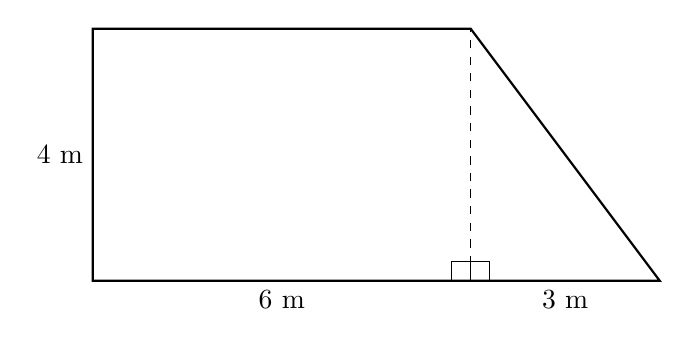
\begin{tikzpicture}[scale=0.8]
\draw[thick] (0,0) -- (6,0) -- (9,0) -- (6,4) -- (0,4) -- cycle;
\draw[dashed] (6,0) -- (6,4);
\draw (6,0) rectangle (5.7,0.3);
\draw (6,0) rectangle (6.3,0.3);
\node[below] at (3,0) {$6$ m};
\node[below] at (7.5,0) {$3$ m};
\node[left] at (0,2) {$4$ m};
\end{tikzpicture}
\end{center}
\begin{enumerate}[label=\textbf{(\alph*)}, leftmargin=*]
\item Calculate the total area of the floor.
\examanswerslot{2cm}{0.25}{2}
\item The cost to carpet the floor is $15$ GBP per square metre. Calculate the total cost to carpet the floor.
\examanswerslot{2cm}{0.25}{2}
\end{enumerate}
\vspace{1cm}\par\noindent\rule{\linewidth}{0.4pt}\vspace{1cm}
\item \needspace{5cm}
The diagram shows a trapezium. \\
\begin{center}
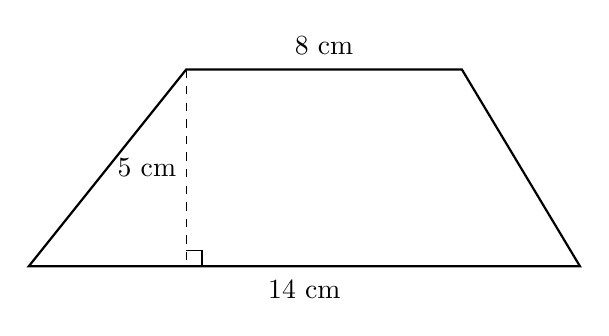
\begin{tikzpicture}
\draw[thick] (0,0) -- (7,0) -- (5.5,2.5) -- (2,2.5) -- cycle;
\draw[dashed] (2,2.5) -- (2,0);
\draw (2,0.2) -- (2.2,0.2) -- (2.2,0);
\node at (3.5,-0.3) {$14$ cm};
\node at (3.75,2.8) {$8$ cm};
\node at (1.5,1.25) {$5$ cm};
\end{tikzpicture}
\end{center}
\begin{enumerate}[label=\textbf{(\alph*)}, leftmargin=*]
\item Calculate the area of the trapezium.
\examanswerslot{2cm}{0.25}{2}
\item A distinct triangle has the same area as the trapezium.
The triangle has a base of $11$ cm and a perpendicular height of $h$ cm. \\
\par\vspace{0.1cm}\hspace*{0.6cm}$\text{Area} = \dfrac{1}{2} \times \text{base} \times \text{height}$\par\vspace{0.15cm}
Show that the height, $h$, of the triangle is $10$ cm. \\
\examanswerslot{3.5cm}{0}{2}
\end{enumerate}
\vspace{1cm}\par\noindent\rule{\linewidth}{0.4pt}\vspace{1cm}
\item \needspace{5cm}
A rectangle has length $9$ cm and width $4$ cm. \\
A square has the exact same area as the rectangle. \\
\begin{center}
\begin{tikzpicture}
\draw[thick] (0,0) rectangle (4.5,2);
\node at (2.25,-0.3) {$9$ cm};
\node at (5.1,1) {$4$ cm};
\draw[thick] (7,0) rectangle (10,3);
\end{tikzpicture}
\end{center}
\begin{enumerate}[label=\textbf{(\alph*)}, leftmargin=*]
\item Calculate the area of the rectangle.
\examanswerslot{2cm}{0.25}{1}
\item Find the side length of the square.
\examanswerslot{2cm}{0.25}{2}
\item Calculate the perimeter of the square.
\examanswerslot{2cm}{0.25}{1}
\end{enumerate}
\vspace{1cm}\par\noindent\rule{\linewidth}{0.4pt}\vspace{1cm}
\item \needspace{5cm}
The diagram shows a parallelogram. \\
\begin{center}
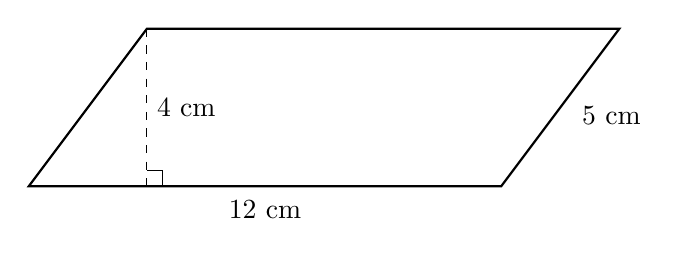
\begin{tikzpicture}
\draw[thick] (0,0) -- (6,0) -- (7.5,2) -- (1.5,2) -- cycle;
\draw[dashed] (1.5,2) -- (1.5,0);
\draw (1.5,0.2) -- (1.7,0.2) -- (1.7,0);
\node at (3,-0.3) {$12$ cm};
\node at (2,1) {$4$ cm};
\node at (7.4,0.9) {$5$ cm};
\end{tikzpicture}
\end{center}
\begin{enumerate}[label=\textbf{(\alph*)}, leftmargin=*]
\item Calculate the perimeter of the parallelogram.
\examanswerslot{2cm}{0.25}{1}
\item Calculate the area of the parallelogram.
\examanswerslot{2cm}{0.25}{1}
\end{enumerate}
\vspace{1cm}\par\noindent\rule{\linewidth}{0.4pt}\vspace{1cm}
\item \needspace{5cm}
The diagram shows a trapezium. \\
\begin{center}
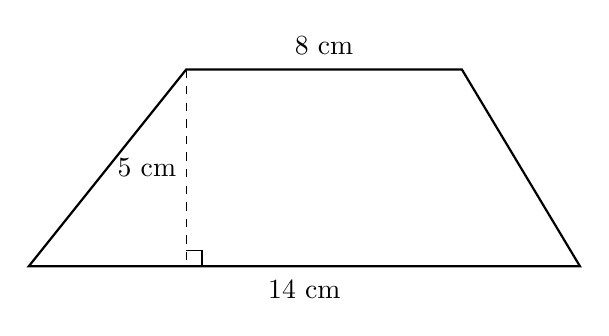
\begin{tikzpicture}
\draw[thick] (0,0) -- (7,0) -- (5.5,2.5) -- (2,2.5) -- cycle;
\draw[dashed] (2,2.5) -- (2,0);
\draw (2,0.2) -- (2.2,0.2) -- (2.2,0);
\node at (3.5,-0.3) {$14$ cm};
\node at (3.75,2.8) {$8$ cm};
\node at (1.5,1.25) {$5$ cm};
\end{tikzpicture}
\end{center}
\begin{enumerate}[label=\textbf{(\alph*)}, leftmargin=*]
\item Calculate the area of the trapezium.
\examanswerslot{2cm}{0.25}{2}
\item A distinct triangle has the same area as the trapezium.
The triangle has a base of $11$ cm and a perpendicular height of $h$ cm. \\
\par\vspace{0.1cm}\hspace*{0.6cm}$\text{Area} = \dfrac{1}{2} \times \text{base} \times \text{height}$\par\vspace{0.15cm}
Show that the height, $h$, of the triangle is $10$ cm. \\
\examanswerslot{3.5cm}{0}{2}
\end{enumerate}
\vspace{1cm}\par\noindent\rule{\linewidth}{0.4pt}\vspace{1cm}
\item \needspace{5cm}
The diagram shows a composite L-shaped polygon. \\
All internal angles are right angles. \\
\begin{center}
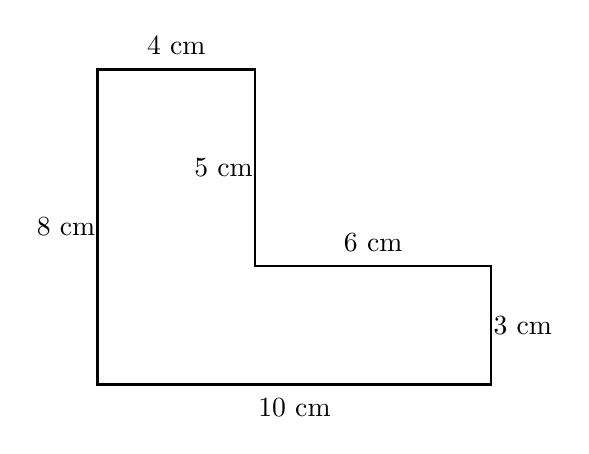
\begin{tikzpicture}
\draw[thick] (0,0) -- (5,0) -- (5,1.5) -- (2,1.5) -- (2,4) -- (0,4) -- cycle;
\node at (2.5,-0.3) {$10$ cm};
\node at (5.4,0.75) {$3$ cm};
\node at (3.5,1.8) {$6$ cm};
\node at (1.6,2.75) {$5$ cm};
\node at (1,4.3) {$4$ cm};
\node at (-0.4,2) {$8$ cm};
\end{tikzpicture}
\end{center}
\begin{enumerate}[label=\textbf{(\alph*)}, leftmargin=*]
\item Calculate the perimeter of the polygon.
\examanswerslot{2cm}{0.25}{1}
\item Calculate the total area of the polygon.
\examanswerslot{2cm}{0.25}{3}
\end{enumerate}
\vspace{1cm}\par\noindent\rule{\linewidth}{0.4pt}\vspace{1cm}
\item \needspace{5cm}
An isosceles triangle and a rectangle are shown below. \\
\begin{center}
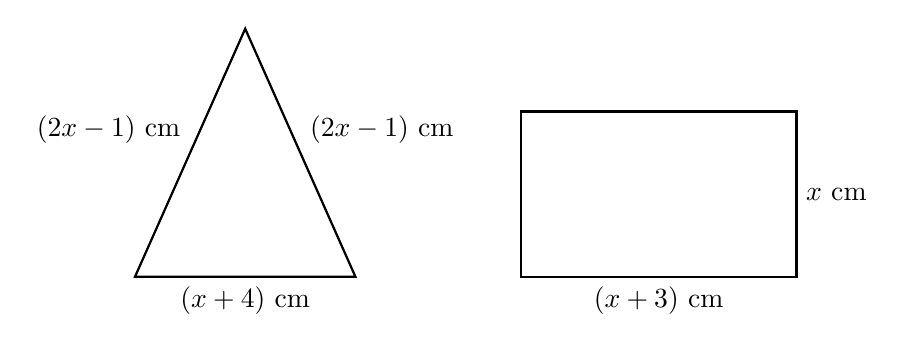
\begin{tikzpicture}[scale=0.7]
\draw[thick] (0,0) -- (4,0) -- (2,4.5) -- cycle;
\node[below] at (2,0) {$(x+4)\text{ cm}$};
\node[above left] at (1,2.25) {$(2x-1)\text{ cm}$};
\node[above right] at (3,2.25) {$(2x-1)\text{ cm}$};
\begin{scope}[shift={(7,0)}]
\draw[thick] (0,0) rectangle (5,3);
\node[below] at (2.5,0) {$(x+3)\text{ cm}$};
\node[right] at (5,1.5) {$x\text{ cm}$};
\end{scope}
\end{tikzpicture}
\end{center}
The perimeter of the triangle is equal to the perimeter of the rectangle. \\
\begin{enumerate}[label=\textbf{(\alph*)}, leftmargin=*]
\item Show that the equation simplifies to find $x = 4$.
\examanswerslot{4cm}{0}{3}
\item Calculate the area of the rectangle.
\examanswerslot{2cm}{0.25}{2}
\end{enumerate}
\vspace{1cm}\par\noindent\rule{\linewidth}{0.4pt}\vspace{1cm}
\item \needspace{5cm}
The diagram shows a composite shape formed by joining a square and a right-angled triangle. \\
\begin{center}
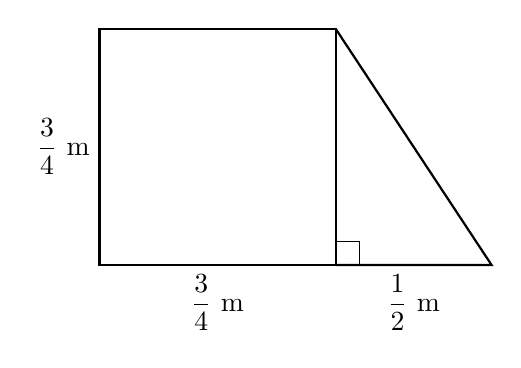
\begin{tikzpicture}[scale=3]
\draw[thick] (0,0) rectangle (1,1);
\draw[thick] (1,0) -- (1.66,0) -- (1,1);
\draw (1,0) rectangle (1.1,0.1);
\node[left] at (0,0.5) {$\dfrac{3}{4}\text{ m}$};
\node[below] at (0.5,0) {$\dfrac{3}{4}\text{ m}$};
\node[below] at (1.33,0) {$\dfrac{1}{2}\text{ m}$};
\end{tikzpicture}
\end{center}
\noindent Calculate the exact total area of the composite shape. Give your answer as a single fraction in its simplest form. \par\vspace{0.1cm}
\examanswerslot{3.5cm}{0.25}{4}
\vspace{1cm}\par\noindent\rule{\linewidth}{0.4pt}\vspace{1cm}
\item \needspace{5cm}
A parallelogram is shown below. \\
\begin{center}
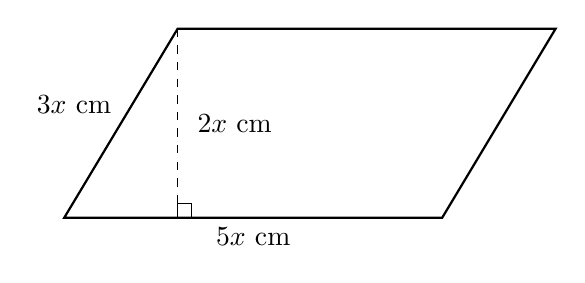
\begin{tikzpicture}[scale=0.6]
\draw[thick] (0,0) -- (8,0) -- (10.4,4) -- (2.4,4) -- cycle;
\draw[dashed] (2.4,4) -- (2.4,0);
\draw (2.4,0) rectangle (2.7,0.3);
\node[below] at (4,0) {$5x\text{ cm}$};
\node[left] at (4.6,2) {$2x\text{ cm}$};
\node[above left] at (1.2,2) {$3x\text{ cm}$};
\end{tikzpicture}
\end{center}
The area of the parallelogram is $40\text{ cm}^2$. \\
\begin{enumerate}[label=\textbf{(\alph*)}, leftmargin=*]
\item Calculate the value of $x$, given that $x > 0$.
\examanswerslot{3cm}{0.25}{3}
\item Calculate the perimeter of the parallelogram.
\examanswerslot{2cm}{0.25}{2}
\end{enumerate}
\vspace{1cm}\par\noindent\rule{\linewidth}{0.4pt}\vspace{1cm}
\item \needspace{5cm}
A rectangle and a trapezium are shown below. \\
\begin{center}
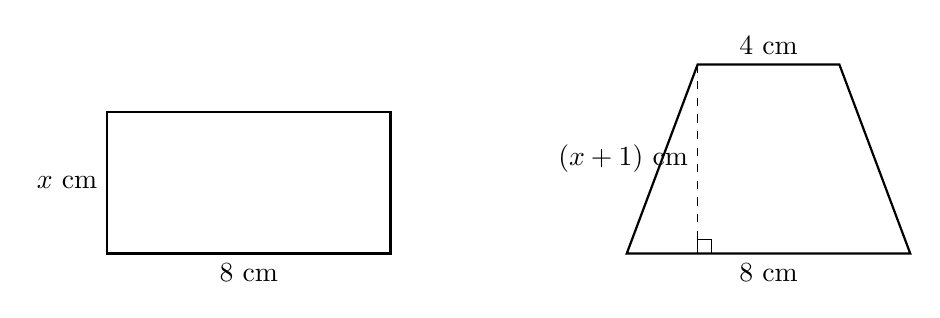
\begin{tikzpicture}[scale=0.6]
\begin{scope}[shift={(-3,0)}]
\draw[thick] (0,0) rectangle (6,3);
\node[below] at (3,0) {$8\text{ cm}$};
\node[left] at (0,1.5) {$x\text{ cm}$};
\end{scope}
\begin{scope}[shift={(8,0)}]
\draw[thick] (0,0) -- (6,0) -- (4.5,4) -- (1.5,4) -- cycle;
\draw[dashed] (1.5,4) -- (1.5,0);
\draw (1.5,0) rectangle (1.8,0.3);
\node[below] at (3,0) {$8\text{ cm}$};
\node[above] at (3,4) {$4\text{ cm}$};
\node[left] at (1.5,2) {$(x+1)\text{ cm}$};
\end{scope}
\end{tikzpicture}
\end{center}
The area of the rectangle is equal to the area of the trapezium. \\
\begin{enumerate}[label=\textbf{(\alph*)}, leftmargin=*]
\item Find the value of $x$.
\examanswerslot{3cm}{0.25}{3}
\item Calculate the perimeter of the rectangle.
\examanswerslot{2cm}{0.25}{1}
\end{enumerate}
\vspace{1cm}\par\noindent\rule{\linewidth}{0.4pt}\vspace{1cm}
\item \needspace{5cm}
A rectangle is shown below. All dimensions are in centimetres. \\
\begin{center}
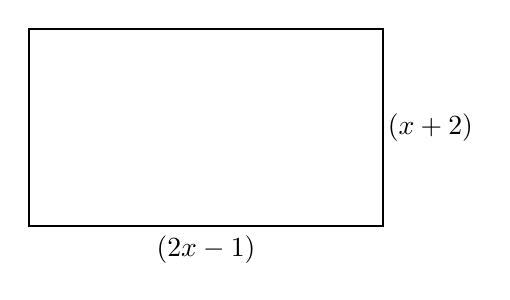
\begin{tikzpicture}
\draw [thick] (0,0) rectangle (4.5,2.5);
\node at (2.25,-0.3) {$(2x - 1)$};
\node at (5.1,1.25) {$(x + 2)$};
\end{tikzpicture}
\end{center}
The exact area of the rectangle is $18$ cm$^2$. \\
\begin{enumerate}[label=\textbf{(\alph*)}, leftmargin=*]
\item Show that the area equation simplifies to:
\par\vspace{0.1cm}\hspace*{0.6cm}$2x^2 + 3x - 20 = 0$\par\vspace{0.15cm}
\examanswerslot{3.5cm}{0}{2}
\item Solve the equation to find the value of $x$.
\examanswerslot{2cm}{0.25}{3}
\item Calculate the exact perimeter of the rectangle.
\examanswerslot{2cm}{0.25}{2}
\end{enumerate}
\vspace{1cm}\par\noindent\rule{\linewidth}{0.4pt}\vspace{1cm}
\item \needspace{5cm}
The coordinates of the vertices of a polygon are $A(1, 1)$, $B(5, 1)$, $C(7, 5)$, and $D(3, 5)$. \\
\begin{enumerate}[label=\textbf{(\alph*)}, leftmargin=*]
\item On the grid provided, draw the parallelogram $ABCD$.
\begin{center}
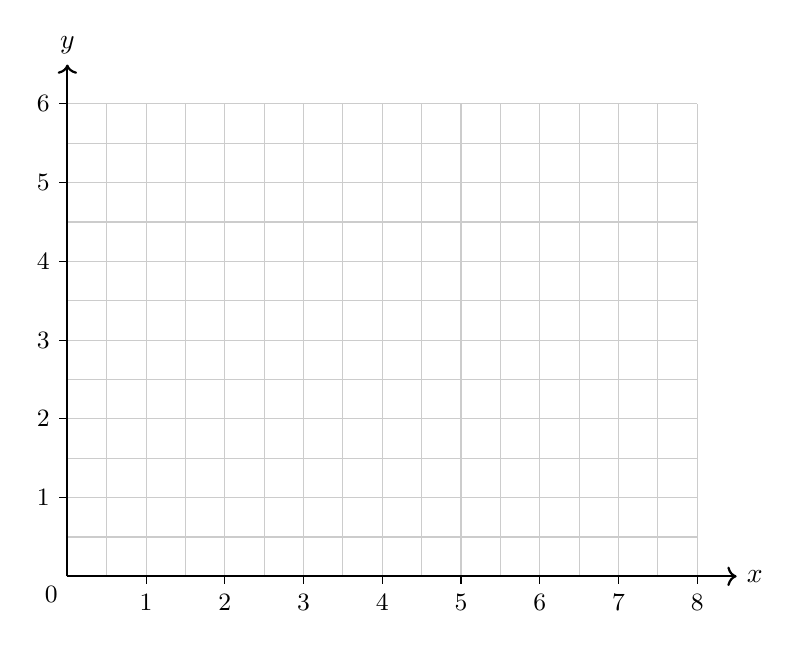
\begin{tikzpicture}
\draw [color=gray!40, xstep=0.5cm, ystep=0.5cm] (0,0) grid (8,6);
\draw [thick, ->] (0,0) -- (8.5,0) node[right] {$x$};
\draw [thick, ->] (0,0) -- (0,6.5) node[above] {$y$};
\foreach \x [evaluate=\x as \val using int(\x)] in {1,2,3,4,5,6,7,8} {
\draw (\x,0) -- (\x,-0.1) node[below] {\small $\val$};
}
\foreach \y [evaluate=\y as \val using int(\y)] in {1,2,3,4,5,6} {
\draw (0,\y) -- (-0.1,\y) node[left] {\small $\val$};
}
\node[below left] at (0,0) {\small $0$};
\end{tikzpicture}
\end{center}
\phantom{.} \hfill \makebox[15pt][r]{[2]}
\item Calculate the exact area of the parallelogram $ABCD$.
\examanswerslot{2cm}{0.25}{2}
\item Calculate the exact perimeter of the parallelogram $ABCD$. Give your answer in the form $p + q\sqrt{r}$ where $p, q$, and $r$ are integers.
\examanswerslot{2cm}{0.25}{3}
\end{enumerate}
\vspace{1cm}\par\noindent\rule{\linewidth}{0.4pt}\vspace{1cm}
\item \needspace{5cm}
The parallel sides of a trapezium are in the ratio $3 : 5$. \\
\begin{center}
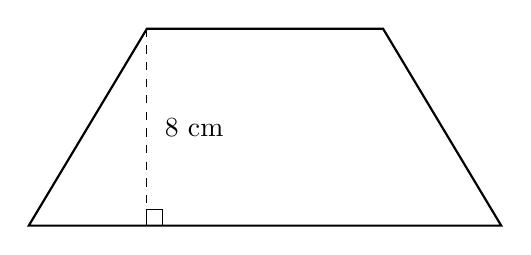
\begin{tikzpicture}
\draw [thick] (1.5,2.5) -- (4.5,2.5) -- (6,0) -- (0,0) -- cycle;
\draw [dashed] (1.5,2.5) -- (1.5,0);
\draw (1.5,0) rectangle (1.7,0.2);
\node at (2.1,1.25) {$8$ cm};
\end{tikzpicture}
\end{center}
The perpendicular height of the trapezium is $8$ cm. \\
The area of the trapezium is $96$ cm$^2$. \\
\begin{enumerate}[label=\textbf{(\alph*)}, leftmargin=*]
\item Calculate the lengths of the two parallel sides.
\examanswerslot{2cm}{0.25}{3}
\item The trapezium is isosceles. Calculate the exact perimeter of the trapezium. Give your answer in the form $p + q\sqrt{r}$ where $p, q$, and $r$ are integers.
\examanswerslot{2cm}{0.25}{4}
\end{enumerate}
\vspace{1cm}\par\noindent\rule{\linewidth}{0.4pt}\vspace{1cm}
\item \needspace{5cm}
The diagram shows a parallelogram with a base of $15.4$ cm and a slant edge of $8.7$ cm. The perpendicular height of the parallelogram is $7.2$ cm. \\
\begin{center}
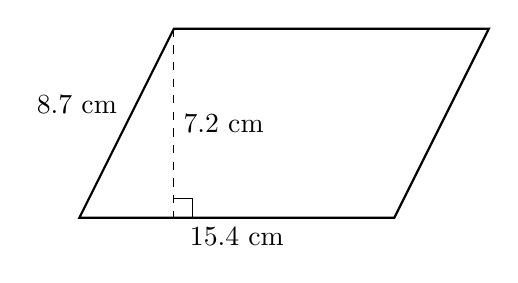
\begin{tikzpicture}[scale=0.8]
\draw[thick] (0,0) -- (5,0) -- (6.5,3) -- (1.5,3) -- cycle;
\draw[dashed] (1.5,3) -- (1.5,0);
\draw (1.5,0.3) -- (1.8,0.3) -- (1.8,0);
\node[below] at (2.5,0) {$15.4$ cm};
\node[above left] at (0.75,1.5) {$8.7$ cm};
\node[right] at (1.5,1.5) {$7.2$ cm};
\end{tikzpicture}
\end{center}
\noindent A student is analysing the geometric properties of the shape. \par\vspace{0.1cm}
\begin{enumerate}[label=\textbf{(\alph*)}, leftmargin=*]
\item Calculate the perimeter of the parallelogram.
\examanswerslot{2cm}{0.25}{2}
\item Calculate the area of the parallelogram.
\examanswerslot{2cm}{0.25}{2}
\end{enumerate}
\vspace{1cm}\par\noindent\rule{\linewidth}{0.4pt}\vspace{1cm}
\item \needspace{5cm}
The diagram shows a trapezium. The parallel sides have lengths of $18.2$ m and $12.5$ m. The perpendicular distance between the parallel sides is $6.4$ m. The lengths of the remaining two sides are $7.1$ m and $8.5$ m. \\
\begin{center}
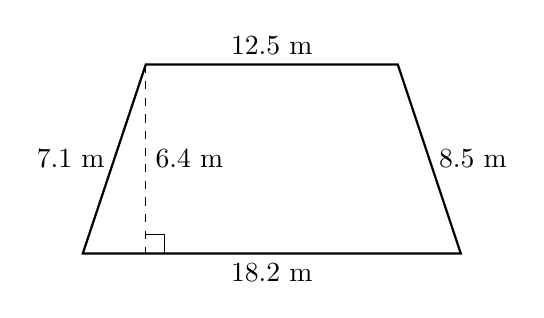
\begin{tikzpicture}[scale=0.8]
\draw[thick] (0,0) -- (6,0) -- (5,3) -- (1,3) -- cycle;
\draw[dashed] (1,3) -- (1,0);
\draw (1,0.3) -- (1.3,0.3) -- (1.3,0);
\node[below] at (3,0) {$18.2$ m};
\node[above] at (3,3) {$12.5$ m};
\node[left] at (0.5,1.5) {$7.1$ m};
\node[right] at (5.5,1.5) {$8.5$ m};
\node[right] at (1,1.5) {$6.4$ m};
\end{tikzpicture}
\end{center}
\begin{enumerate}[label=\textbf{(\alph*)}, leftmargin=*]
\item Calculate the perimeter of the trapezium.
\examanswerslot{2cm}{0.25}{2}
\item Calculate the area of the trapezium.
\examanswerslot{2cm}{0.25}{2}
\end{enumerate}
\vspace{1cm}\par\noindent\rule{\linewidth}{0.4pt}\vspace{1cm}
\item \needspace{5cm}
The diagram shows a compound shape consisting of a rectangle and a right-angled triangle. The rectangle has a length of $14.2$ cm and a width of $9.5$ cm. The triangle has a perpendicular height of $5.3$ cm. \\
\begin{center}
\begin{tikzpicture}[scale=0.8]
\draw[thick] (0,0) -- (4,0) -- (4,3) -- (0,3) -- cycle;
\draw[thick] (0,3) -- (2,5) -- (4,3);
\draw[dashed] (2,5) -- (2,3);
\draw (2,3) -- (2.3,3) -- (2.3,3.3) -- (2,3.3);
\node[below] at (2,0) {$14.2$ cm};
\node[left] at (0,1.5) {$9.5$ cm};
\node[right] at (2,4) {$5.3$ cm};
\end{tikzpicture}
\end{center}
\begin{enumerate}[label=\textbf{(\alph*)}, leftmargin=*]
\item Calculate the total area of the compound shape.
\examanswerslot{2cm}{0.25}{3}
\item A protective liquid coating is applied to the surface of the shape. The cost of the coating is $0.15$ USD per square centimetre. Calculate the total cost of the coating.
\examanswerslot{2cm}{0.25}{2}
\end{enumerate}
\vspace{1cm}\par\noindent\rule{\linewidth}{0.4pt}\vspace{1cm}
\item \needspace{5cm}
The diagram shows a right-angled triangle. The base length is $11.4$ cm and the hypotenuse is $15.6$ cm. \\
\begin{center}
\begin{tikzpicture}[scale=0.8]
\draw[thick] (0,0) -- (4,0) -- (0,4) -- cycle;
\draw (0.3,0) -- (0.3,0.3) -- (0,0.3);
\node[below] at (2,0) {$11.4$ cm};
\node[above right] at (2,2) {$15.6$ cm};
\end{tikzpicture}
\end{center}
\begin{enumerate}[label=\textbf{(\alph*)}, leftmargin=*]
\item Calculate the perpendicular height of the right-angled triangle.
\examanswerslot{2cm}{0.25}{3}
\item The formula for the area of a triangle is:
\par\vspace{0.1cm}\hspace*{0.6cm}$ Area = \dfrac{1}{2}bh $\par\vspace{0.15cm}
Calculate the area of the triangle. \\
\examanswerslot{2cm}{0.25}{2}
\end{enumerate}
\vspace{1cm}\par\noindent\rule{\linewidth}{0.4pt}\vspace{1cm}
\item \needspace{5cm}
The diagram shows a symmetrical trapezium with parallel sides of length $10.8$ mm and $x$ mm. The perpendicular height is $5.2$ mm and the two slant sides are each $7.5$ mm in length. \\
\begin{center}
\begin{tikzpicture}[scale=0.8]
\draw[thick] (0,0) -- (6,0) -- (4.5,2.5) -- (1.5,2.5) -- cycle;
\draw[dashed] (1.5,2.5) -- (1.5,0);
\draw (1.5,0.3) -- (1.8,0.3) -- (1.8,0);
\node[below] at (3,0) {$x$ mm};
\node[above] at (3,2.5) {$10.8$ mm};
\node[right] at (1.5,1.25) {$5.2$ mm};
\node[left] at (0.75,1.25) {$7.5$ mm};
\node[right] at (5.25,1.25) {$7.5$ mm};
\end{tikzpicture}
\end{center}
The total area of the trapezium is $85.8$ mm$^2$. The formula for the area of a trapezium is: \\
\par\vspace{0.1cm}\hspace*{0.6cm}$ A = \dfrac{1}{2}(a+b)h $\par\vspace{0.15cm}
\begin{enumerate}[label=\textbf{(\alph*)}, leftmargin=*]
\item Show that the value of $x$ is $22.2$.
\examanswerslot{3.5cm}{0}{2}
\item Calculate the perimeter of the trapezium.
\examanswerslot{2cm}{0.25}{2}
\end{enumerate}
\vspace{1cm}\par\noindent\rule{\linewidth}{0.4pt}\vspace{1cm}
\item \needspace{5cm}
The diagram shows a trapezium $ABCD$. $AB$ is parallel to $DC$. Angle $ADC = 90^\circ$. \\
$AB = 12.4$ cm, $DC = 18.2$ cm, and $BC = 8.5$ cm. \\
\begin{center}
\begin{tikzpicture}[scale=0.35]
\coordinate (A) at (0, 6.21);
\coordinate (B) at (12.4, 6.21);
\coordinate (C) at (18.2, 0);
\coordinate (D) at (0, 0);
\draw[thick] (A) -- (B) -- (C) -- (D) -- cycle;
\draw (0, 0.7) -- (0.7, 0.7) -- (0.7, 0);
\draw (0, 5.51) -- (0.7, 5.51) -- (0.7, 6.21);
\node[above] at (6.2, 6.21) {$12.4$ cm};
\node[below] at (9.1, 0) {$18.2$ cm};
\node[right] at (15.3, 3.1) {$8.5$ cm};
\node[above left] at (A) {$A$};
\node[above right] at (B) {$B$};
\node[below right] at (C) {$C$};
\node[below left] at (D) {$D$};
\node[below, gray] at (9.1, -1.5) {Not to scale};
\end{tikzpicture}
\end{center}
\begin{enumerate}[label=\textbf{(\alph*)}, leftmargin=*]
\item Calculate the perimeter of the trapezium $ABCD$.
\examanswerslot{2cm}{0.25}{3}
\item Calculate the area of the trapezium $ABCD$.
\examanswerslot{2cm}{0.25}{2}
\end{enumerate}
\vspace{1cm}\par\noindent\rule{\linewidth}{0.4pt}\vspace{1cm}
\item \needspace{5cm}
The diagram shows a parallelogram. The base is $(3x + 2)$ cm and the perpendicular height is $(x + 1)$ cm. The slant edge is $(2x + 1.5)$ cm. \\
The area of the parallelogram is $56$ cm$^2$. \\
\begin{center}
\begin{tikzpicture}[scale=0.7]
\coordinate (A) at (0,0);
\coordinate (B) at (6,0);
\coordinate (C) at (7,3);
\coordinate (D) at (1,3);
\draw[thick] (A) -- (B) -- (C) -- (D) -- cycle;
\draw[dashed] (D) -- (1,0);
\draw (1, 0.3) -- (1.3, 0.3) -- (1.3, 0);
\node[below] at (3,0) {$(3x + 2)$ cm};
\node[right] at (1,1.5) {$(x + 1)$ cm};
\node[above left] at (0.5, 1.5) {$(2x + 1.5)$ cm};
\node[below, gray] at (3.5, -1) {Not to scale};
\end{tikzpicture}
\end{center}
\begin{enumerate}[label=\textbf{(\alph*)}, leftmargin=*]
\item Show that $x$ satisfies the equation
\par\vspace{0.1cm}\hspace*{0.6cm}$3x^2 + 5x - 54 = 0$\par\vspace{0.15cm}
\examanswerslot{3.5cm}{0}{2}
\item Solve the equation $3x^2 + 5x - 54 = 0$ to find the value of $x$. Give your answer correct to 3 significant figures.
\examanswerslot{2cm}{0.25}{3}
\item Calculate the perimeter of the parallelogram.
\examanswerslot{2cm}{0.25}{2}
\end{enumerate}
\vspace{1cm}\par\noindent\rule{\linewidth}{0.4pt}\vspace{1cm}
\item \needspace{5cm}
A metal plate is formed from a rectangle $ABCD$ and an isosceles triangle $ABE$. \\
$AB = 10.5$ cm and $BC = 14.8$ cm. The perpendicular height of the triangle $ABE$ from the base $AB$ is $6.5$ cm. \\
\begin{center}
\begin{tikzpicture}[scale=0.35]
\coordinate (D) at (0,0);
\coordinate (C) at (10.5,0);
\coordinate (B) at (10.5,14.8);
\coordinate (A) at (0,14.8);
\coordinate (E) at (5.25,21.3);
\draw[thick] (D) -- (C) -- (B) -- (E) -- (A) -- cycle;
\draw[dashed] (A) -- (B);
\draw[dashed] (E) -- (5.25,14.8);
\draw (5.25, 15.5) -- (5.95, 15.5) -- (5.95, 14.8);
\node[below] at (5.25, 0) {$10.5$ cm};
\node[right] at (10.5, 7.4) {$14.8$ cm};
\node[right] at (5.25, 18.05) {$6.5$ cm};
\node[below left] at (D) {$D$};
\node[below right] at (C) {$C$};
\node[above right] at (B) {$B$};
\node[above left] at (A) {$A$};
\node[above] at (E) {$E$};
\node[below, gray] at (5.25, -2) {Not to scale};
\end{tikzpicture}
\end{center}
\begin{enumerate}[label=\textbf{(\alph*)}, leftmargin=*]
\item Calculate the total area of the metal plate.
\examanswerslot{2cm}{0.25}{3}
\item Calculate the perimeter of the metal plate.
\examanswerslot{2cm}{0.25}{3}
\end{enumerate}
\vspace{1cm}\par\noindent\rule{\linewidth}{0.4pt}\vspace{1cm}
\item \needspace{5cm}
A rectangular piece of card measures $32.0$ cm by $24.0$ cm. A hole in the shape of an isosceles trapezium is cut from the centre of the card, leaving the shaded region shown in the diagram. \\
The parallel sides of the trapezium are $12.5$ cm and $18.5$ cm. The perpendicular height of the trapezium is $8.4$ cm. \\
\begin{center}
\begin{tikzpicture}[scale=0.25]
\draw[thick, fill=gray!20] (0,0) rectangle (32,24);
\coordinate (T1) at (9.75, 7.8);
\coordinate (T2) at (22.25, 7.8);
\coordinate (T3) at (25.25, 16.2);
\coordinate (T4) at (6.75, 16.2);
\draw[thick, fill=white] (T1) -- (T2) -- (T3) -- (T4) -- cycle;
\draw[dashed] (16, 7.8) -- (16, 16.2);
\node[below] at (16,0) {$32.0$ cm};
\node[left] at (0,12) {$24.0$ cm};
\node[below] at (16, 7.8) {$12.5$ cm};
\node[above] at (16, 16.2) {$18.5$ cm};
\node[right] at (16, 12) {$8.4$ cm};
\node[below, gray] at (16, -2) {Not to scale};
\end{tikzpicture}
\end{center}
\begin{enumerate}[label=\textbf{(\alph*)}, leftmargin=*]
\item Calculate the area of the shaded region.
\examanswerslot{2cm}{0.25}{3}
\item Calculate the perimeter of the cut-out isosceles trapezium.
\examanswerslot{2cm}{0.25}{3}
\item The shaded region is painted. The cost of the paint is $0.045$ EUR per square centimetre. Calculate the total cost of painting the shaded region.
\examanswerslot{2cm}{0.25}{2}
\end{enumerate}
\vspace{1cm}\par\noindent\rule{\linewidth}{0.4pt}\vspace{1cm}
\item \needspace{5cm}
A cross-section of a solid is formed by a rectangle $ABCD$ and an isosceles trapezium $DCEF$ placed adjacent to $DC$. \\
The width of the rectangle is $AB = 12.4$ cm and the height is $BC = 5.2$ cm. \\
The top edge of the trapezium $EF$ is parallel to $DC$ and $EF = 7.8$ cm. \\
The total area of the composite cross-section is $98.82$ cm$^2$. \\
\begin{center}
\begin{tikzpicture}[scale=0.7]
\draw[thick] (0,0) -- (6.2,0) node[midway, below] {$12.4$ cm} -- (6.2, 2.6) node[midway, right] {$5.2$ cm} -- (0, 2.6) -- cycle;
\draw[thick] (0,2.6) -- (1.15, 4.3) -- (5.05, 4.3) node[midway, above] {$7.8$ cm} -- (6.2, 2.6);
\draw[dashed] (1.15, 2.6) -- (1.15, 4.3);
\node at (1.15, 3.45) [left] {$h$};
\node at (-0.3, 0) {$A$};
\node at (6.5, 0) {$B$};
\node at (6.5, 2.6) {$C$};
\node at (-0.3, 2.6) {$D$};
\node at (1.15, 4.6) {$E$};
\node at (5.05, 4.6) {$F$};
\node at (3.1, -1) {NOT TO SCALE};
\end{tikzpicture}
\end{center}
\begin{enumerate}[label=\textbf{(\alph*)}, leftmargin=*]
\item Show that the perpendicular height $h$ of the trapezium $DCEF$ is $3.4$ cm.
\examanswerslot{3.5cm}{0}{2}
\item Calculate the total perimeter of the cross-section.
\examanswerslot{2cm}{0.25}{4}
\end{enumerate}
\vspace{1cm}\par\noindent\rule{\linewidth}{0.4pt}\vspace{1cm}
\item \needspace{5cm}
A polygon consists of a rectangle and an isosceles triangle joined at their common base. \\
The rectangle has side lengths of $(2x + 3)$ cm and $(x + 4)$ cm. \\
The attached isosceles triangle has a base of $(2x + 3)$ cm and a perpendicular height of $x$ cm. \\
The total area of the entire polygon is $110$ cm$^2$. \\
\begin{center}
\begin{tikzpicture}[scale=0.8]
\draw[thick] (0,2) -- (4,2) node[midway, above] {$(2x + 3)$} -- (4,0) node[midway, right] {$(x + 4)$} -- (0,0) -- cycle;
\draw[thick] (0,0) -- (2,-2) -- (4,0);
\draw[dashed] (2,0) -- (2,-2) node[midway, right] {$x$};
\node at (2, -3) {NOT TO SCALE};
\end{tikzpicture}
\end{center}
\begin{enumerate}[label=\textbf{(\alph*)}, leftmargin=*]
\item Show that $6x^2 + 25x - 196 = 0$.
\examanswerslot{3.5cm}{0}{3}
\item Solve the equation $6x^2 + 25x - 196 = 0$ to find the value of $x$.
\examanswerslot{2cm}{0.25}{2}
\item Hence, calculate the total perimeter of the polygon.
\examanswerslot{2cm}{0.25}{4}
\end{enumerate}
\vspace{1cm}\par\noindent\rule{\linewidth}{0.4pt}\vspace{1cm}
\item \needspace{5cm}
A minor sector of a circle has a radius of $12\text{ cm}$ and an angle of $30^\circ$. \\
The area, $A$, of a sector is determined by the formula: \\
\par\vspace{0.1cm}\hspace*{0.6cm}$A = \dfrac{\theta}{360} \times \pi r^2$\par\vspace{0.15cm}
\begin{center}
\begin{tikzpicture}
\draw[thick] (0,0) -- (6,0) arc[start angle=0, end angle=30, radius=6] -- cycle;
\draw (1,0) arc[start angle=0, end angle=30, radius=1];
\node at (1.5,0.3) {$30^\circ$};
\node[below] at (3,0) {$12\text{ cm}$};
\end{tikzpicture}
\end{center}
\begin{enumerate}[label=\textbf{(\alph*)}, leftmargin=*]
\item Calculate the area of the sector.
\examanswerslot{2cm}{0.25}{2}
\item Find the perimeter of the sector in the form $a + b\pi$, where $a$ and $b$ are integers.
\examanswerslot{2cm}{0.25}{3}
\end{enumerate}
\vspace{1cm}\par\noindent\rule{\linewidth}{0.4pt}\vspace{1cm}
\item \needspace{5cm}
The diagram shows a sector of a circle with centre $O$ and radius $4\text{ cm}$. \\
The angle of the sector is $90^\circ$. \\
\begin{center}
\begin{tikzpicture}
\draw[thick] (0,0) -- (4,0) arc[start angle=0, end angle=90, radius=4] -- cycle;
\draw (0.4,0) -- (0.4,0.4) -- (0,0.4);
\node[below] at (2,0) {$4\text{ cm}$};
\node[left] at (0,2) {$4\text{ cm}$};
\node[below left] at (0,0) {$O$};
\end{tikzpicture}
\end{center}
\begin{enumerate}[label=\textbf{(\alph*)}, leftmargin=*]
\item Calculate the exact area of the sector.
\examanswerslot{2cm}{0.25}{2}
\item Calculate the exact perimeter of the sector.
\examanswerslot{2cm}{0.25}{3}
\end{enumerate}
\vspace{1cm}\par\noindent\rule{\linewidth}{0.4pt}\vspace{1cm}
\item \needspace{5cm}
The diagram shows a sector of a circle with centre $O$ and radius $6\text{ cm}$. \\
The sector angle is $60^\circ$. \\
\begin{center}
\begin{tikzpicture}
\draw[thick] (0,0) -- (6,0) arc[start angle=0, end angle=60, radius=6] -- cycle;
\draw (0.8,0) arc[start angle=0, end angle=60, radius=0.8];
\node at (1.2,0.4) {$60^\circ$};
\node[below] at (3,0) {$6\text{ cm}$};
\node[below left] at (0,0) {$O$};
\end{tikzpicture}
\end{center}
\begin{enumerate}[label=\textbf{(\alph*)}, leftmargin=*]
\item Show that the exact arc length of the minor sector is $2\pi\text{ cm}$.
\examanswerslot{3.5cm}{0}{2}
\item Calculate the exact area of the major sector in terms of $\pi$.
\examanswerslot{2cm}{0.25}{2}
\end{enumerate}
\vspace{1cm}\par\noindent\rule{\linewidth}{0.4pt}\vspace{1cm}
\item \needspace{5cm}
The diagram shows a semicircle with a straight diameter of $10\text{ cm}$. \\
\begin{center}
\begin{tikzpicture}
\draw[thick] (-5,0) -- (5,0);
\draw[thick] (5,0) arc[start angle=0, end angle=180, radius=5];
\node[below] at (0,0) {$10\text{ cm}$};
\draw[dashed] (0,0) -- (0,0.2);
\end{tikzpicture}
\end{center}
\begin{enumerate}[label=\textbf{(\alph*)}, leftmargin=*]
\item Calculate the exact area of the semicircle.
\examanswerslot{2cm}{0.25}{2}
\item Calculate the total perimeter of the semicircle, leaving your answer in terms of $\pi$.
\examanswerslot{2cm}{0.25}{2}
\end{enumerate}
\vspace{1cm}\par\noindent\rule{\linewidth}{0.4pt}\vspace{1cm}
\item \needspace{5cm}
A ceremonial badge is shaped as a major sector of a circle with centre $O$ and radius $3\text{ cm}$. \\
The reflex angle of the major sector is $240^\circ$. \\
\begin{center}
\begin{tikzpicture}
\draw[thick] (0,0) -- (3,0) arc[start angle=0, end angle=240, radius=3] -- cycle;
\draw (0.5,0) arc[start angle=0, end angle=240, radius=0.5];
\node at (0.8,0.8) {$240^\circ$};
\node[below] at (1.5,0) {$3\text{ cm}$};
\node[below left] at (0,0) {$O$};
\end{tikzpicture}
\end{center}
\begin{enumerate}[label=\textbf{(\alph*)}, leftmargin=*]
\item Show that the exact area of the badge is $6\pi\text{ cm}^2$.
\examanswerslot{3.5cm}{0}{2}
\item The badge is coated in liquid silver. The silver coating process costs $5\text{ GBP}$ per $\pi\text{ cm}^2$.
\begin{enumerate}[label=\textbf{(\roman*)}, leftmargin=0.6cm]
\item Calculate the total cost to coat the badge.
\examanswerslot{2cm}{0.25}{2}
\end{enumerate}
\end{enumerate}
\end{enumerate}

\end{document}
